\documentclass[11pt]{amsart}

\usepackage{amssymb}
\usepackage{mathtools}
\usepackage{microtype}
\usepackage{enumitem}
\usepackage{mathrsfs}
\usepackage{booktabs}
\usepackage{array}
\usepackage{graphicx}
\usepackage{xcolor}
\usepackage{tikz}
\usetikzlibrary{decorations.pathreplacing}
\usepackage[hidelinks]{hyperref}
\hypersetup{pdftitle={Resolution of the ENO-TV conjecture: a parity dichotomy}, pdfauthor={Zhuoyun Li and Kailiang Wu}, pdfsubject={Sharp parity classification and mesh dependence for ENO entropy-source coercivity}, pdfkeywords={ENO reconstruction, ENO-TV conjecture, entropy stability, parity dichotomy, discrete coercivity}}
\emergencystretch=2em


\usepackage[
paperwidth=7in,
paperheight=10in,
left=1in,
right=1in,
top=1in,
bottom=0.9in,
headheight=8pt,
headsep=14pt
]{geometry}


\allowdisplaybreaks
\raggedbottom
\setcounter{tocdepth}{1}

\theoremstyle{plain}
\newtheorem{theorem}{Theorem}[section]
\newtheorem{lemma}[theorem]{Lemma}
\newtheorem{proposition}[theorem]{Proposition}
\newtheorem{corollary}[theorem]{Corollary}
\theoremstyle{definition}
\newtheorem{definition}[theorem]{Definition}
\theoremstyle{remark}
\newtheorem{remark}[theorem]{Remark}
\numberwithin{equation}{section}

\theoremstyle{plain}
\newtheorem{lettertheorem}{Theorem}
\renewcommand{\thelettertheorem}{\Alph{lettertheorem}}


\title[Resolution of the ENO--TV conjecture]{Resolution of the ENO--TV conjecture:\\ a parity dichotomy}

\author[Z. Li]{Zhuoyun Li}
\address[Zhuoyun Li]{Department of Mathematics, Southern University of Science and Technology, Shenzhen, Guangdong 518055, China}

\author[K. Wu]{Kailiang Wu}
\address[Kailiang Wu]{Department of Mathematics and Shenzhen International Center for Mathematics, Southern University of Science and Technology, Shenzhen, Guangdong 518055, China}
\email[Kailiang Wu]{wukl@sustech.edu.cn}
\thanks{Kailiang Wu is the corresponding author. The authors were supported, in part, by the Science Challenge Project (No.~TZ2025007) and the Shenzhen Science and Technology Program (Nos.~JCYJ20250604144300001 and RCJC20221008092757098).}


\subjclass[2020]{Primary 35L65, 65M12, 41A15; Secondary 26D10, 65M08}
\date{}


\begin{document}
	
	
\begin{abstract}
	We resolve the ENO--TV conjecture, a discrete
	coercivity problem in compactness theory for entropy-stable
	approximations of hyperbolic conservation laws.  For order-$k$
	essentially non-oscillatory (ENO) reconstruction from compactly
	supported cell averages, it asks whether the nonnegative ENO source
	times the $(k-1)$st power of the amplitude uniformly controls the
	$(k+1)$st absolute-jump moment.  We prove a parity dichotomy: the
	estimate holds for odd $k\ge3$ and fails for even $k\ge4$; the known
	second-order case completes the classification.  Localization gives
	a selection-independent finite-difference functional uniformly
	comparable to the source and reduces the conjecture to discrete
	interpolation.  For odd orders, summation by parts reveals a hidden
	square; a discrete Gagliardo--Nirenberg inequality yields coercivity.
	For even orders, Euler-polynomial blocks from the functional's
	polynomial kernel yield counterexamples that persist under
	arbitrarily small perturbations making all affected ENO comparisons
	strict.  We also prove two coercive estimates for every $k\ge2$:
	control of jumps larger than a fixed fraction of the amplitude and of
	local blocks modulo sampled polynomials of degree at most $k-2$.
	Via the Cayley--Sylvester decomposition, we compute the dimensions of
	homogeneous first-cohomology spaces for the lattice shift on
	polynomial jump profiles.  At fourth order, for a cubic flux and a
	globally strictly convex entropy, a total-degree-seven component of a
	reduced entropy-flux mismatch represents a nonzero class on profiles
	of degree at most two and hence has no translation-invariant
	finite-stencil $C^7$ local primitive at the zero constant state.
	Odd-order coercivity persists on globally quasi-uniform meshes, whereas for
	each $k\ge2$ it fails on a fixed irregular mesh even though every interface
	contribution remains nonnegative.  This failure is due to the mesh geometry.
\end{abstract}


\maketitle


\tableofcontents

\section{Introduction}\label{sec:intro}


Once shocks form in nonlinear hyperbolic conservation laws, classical
regularity is lost, and weak solutions are often constructed as limits
of regularized approximations.  A priori
estimates, however, may yield only weak compactness, and weak
convergence neither identifies the nonlinear flux in the limit nor
records the fine-scale oscillations of the approximating family. 
The entropy structure recovers what weak convergence loses.  For example,
consider the Cauchy problem for the scalar conservation law
\begin{equation}\label{eq:intro-conservation-law}
	u_t+f(u)_x=0
\end{equation}
with $u(\cdot,0)=u_0\in L^\infty(\mathbb R)$ and
$f\in C^1(\mathbb R)$.  The Kruzhkov entropy inequalities identify
its unique bounded entropy solution \cite{Kruzkov}. 
Under suitable nondegeneracy assumptions on the flux, the kinetic
formulation of Lions, Perthame, and Tadmor \cite{LPT} and the velocity-averaging
theory of Tadmor and Tao \cite{TadmorTao} show how quantitative control of entropy
production yields compactness and fractional regularity. 
 When strong compactness is
unavailable, Young measures record the lost oscillations, and
DiPerna's entropy measure-valued framework incorporates them into the
entropy theory \cite{DiPernaMV}.  
In the scalar case, a bounded entropy measure-valued solution whose
initial Young measure is $\delta_{u_0(x)}$ concentrates on the
Kruzhkov solution \cite{DiPernaMV}. 
 For systems, such concentration need not
occur in general.  For a hyperbolic system endowed with an entropy
that is uniformly strictly convex on the relevant state range,
however, every bounded admissible measure-valued solution with the
same initial data as a Lipschitz solution concentrates on that
solution for as long as the latter exists \cite{BLS}.  
A numerical
convergence argument must therefore recover, at the discrete level, 
enough quantitative control either to identify the scalar entropy
solution or, for systems, to pass consistently to an entropy
measure-valued limit.

The discrete question is the passage from entropy stability to
quantitative coercivity.  
The convergence framework of Fjordholm, K\"appeli, Mishra, and Tadmor
\cite{FKMT} makes this requirement concrete: among its compactness
inputs is a weak BV estimate controlling jumps between neighboring
cell averages.  A discrete
entropy inequality supplies the sign of the dissipation, whereas the
weak BV estimate requires quantitative control of its size. 
A natural candidate for this control is supplied by classical
essentially non-oscillatory (ENO) reconstruction, 
 introduced by Harten, Engquist, Osher, and
Chakravarthy \cite{Harten} in 1987 to retain any prescribed order of accuracy on
smooth data while suppressing spurious oscillations near shocks. On the unit grid $x_{i+1/2}=i+1/2$, let
$\bar u=(\bar u_i)_{i\in\mathbb Z}$ be a compactly supported sequence
of cell averages, with forward difference $(\mathrm Db)_i:=b_{i+1}-b_i$
and jumps $a_i:=(\mathrm D\bar u)_i$; the ENO procedure of order $k$
constructs in each cell a polynomial $p_i^{(k)}$ of degree at most
$k-1$.  Its relevance to the coercivity problem rests on a sign
property proved by Fjordholm, Mishra, and Tadmor (FMT) \cite{FMT}: writing
$\Delta p_{i+1/2}^{(k)}:=p_{i+1}^{(k)}(x_{i+1/2})-p_i^{(k)}(x_{i+1/2})$
for the jump of the reconstructed traces,
\begin{equation}\label{eq:intro-sign-property}
a_i\,\Delta p_{i+1/2}^{(k)}\ge0
\end{equation}
at every interface.  Summing these products yields the ENO source
\begin{equation}\label{eq:intro-Qk}
Q_k(\bar u):=\sum_{i\in\mathbb Z} a_i\,\Delta p_{i+1/2}^{(k)},
\end{equation}
which is therefore nonnegative.  The ENO--TV conjecture \cite{FjordholmHandbook} asserts that
this sign-definite source is quantitatively coercive: for each fixed
$k\ge2$, there is a constant $C_k$ such that every compactly supported
sequence of cell averages satisfies
\begin{equation}\label{eq:full-enotv-intro}
\sum_{i\in\mathbb Z}|a_i|^{k+1}
\le C_k\,\|\bar u\|_{\ell^\infty}^{k-1}\,Q_k(\bar u).
\end{equation}
Despite the historical name ENO--TV, the left-hand side is a
superlinear moment of the cell-average jumps rather than the total
variation itself.  The amplitude factor is forced by homogeneity: the
left-hand side has degree $k+1$ in the data, whereas $Q_k$ has degree
two.  Prior to the present work, the estimate was known only for
$k=2$ \cite[Section~4.4]{FjordholmHandbook}; see also 
\cite[(2.16)]{CFM2AN}.  All cases $k\ge3$ remained
open.  

In this paper, we resolve the conjecture \eqref{eq:full-enotv-intro}
and prove a parity dichotomy above the classical $k=2$ case: the
estimate holds for every odd $k\ge3$, whereas it fails for every even
$k\ge4$.  Together with the known second-order estimate, this
completes the classification.


The conjecture \eqref{eq:full-enotv-intro} remained difficult for the same reason that ENO is
effective near a discontinuity: the stencil is selected adaptively
from the data.  At each stage, ENO compares the absolute values of two
neighboring divided differences, an \emph{ENO comparison}, and extends
the stencil toward the smaller one; the comparison is \emph{strict}
when the two values are unequal.  This adaptivity has made ENO and its
weighted variants (WENO) standard high-resolution methods for
hyperbolic conservation laws \cite{LiuOsherChan,JiangShu,Shu}. The adaptivity is
also precisely what the analysis must confront.  Once all stencil
choices are fixed, the reconstruction is linear in the data and $Q_k$
is a quadratic form.  The comparisons, however, partition the data
space into regions, and crossing a boundary changes both the selected
stencil and the quadratic form.  
Even the local sign property
\eqref{eq:intro-sign-property}, which concerns each interface
separately, was not proved until twenty-six years after ENO was
introduced.  The conjecture \eqref{eq:full-enotv-intro}, by contrast,
seeks a global coercive estimate and requires two further forms of
control: 
the bound must be uniform across all regions and their boundaries, and
it must be global, assembling the interface terms
$a_i\,\Delta p_{i+1/2}^{(k)}$ into a single estimate for
$\sum_i|a_i|^{k+1}$.  It is therefore a global, nonlinear coercivity
problem for an adaptively switching family of discrete dissipations,
rather than a spectral estimate for one fixed operator.

One main new observation is that, despite the adaptive switching, the ENO
source admits a selection-independent localization.  To make this precise, set
\[
A_j^{(k)}:=\max_{0\le s<k}|a_{j+s}|,
\qquad
\mathcal E_k(a):=
\sum_{j\in\mathbb Z}A_j^{(k)}
|\mathrm D^{k-1}a_j|.
\]
We prove, uniformly over all stencil patterns selected by the ENO
rule, that
\begin{equation}\label{eq:intro-selection-free-source}
	Q_k(\bar u)\asymp_k\mathcal E_k(a),
\end{equation}
where the comparison constants depend only on $k$.  This comparison
reduces the conjecture to a discrete interpolation problem on the
integer lattice.  The passage from the local comparison to the global
estimate depends on the parity of $k$.  For odd orders, summation by
parts reveals a hidden square: the localized source controls a
discrete energy, and a discrete Gagliardo--Nirenberg inequality
converts this energy, together with the boundedness of the data, into
the conjectured global estimate.  For even orders, the highest
difference has odd order, so the preceding square identity is
unavailable.  The polynomial kernel of
$\mathrm D^{k-1}$ is present at every order; what is special in even
orders is that its maximal-degree profiles can be concatenated into
long Euler-polynomial blocks for which the jump moment accumulates in
the interiors while the localized source is confined to the junctions
and the two outer endpoints. 
These counterexamples can be chosen so that every ENO comparison
affected by the jump support is strict.  The
selected stencil pattern is then locally constant, and the
quantitative failure persists on an open neighborhood in the
corresponding finite-dimensional data space.  Thus the even-order
failure is structural, not an artifact of tie-breaking.   

This even-order failure, however, does not end the convergence program for high-order 
entropy-stable ENO schemes, such as the TeCNO schemes of Fjordholm,
Mishra, and Tadmor \cite{FMTtecno,FjordholmThesis}, because we
find two weaker coercive estimates that remain valid in every
order.  One controls the jumps larger than a fixed fraction of the
cell-average amplitude; the other controls local jump blocks modulo
the polynomial kernel, the same space from which the counterexamples
are built.  In the companion paper \cite{LiWuCompanion}, we use these estimates to establish the compactness and convergence theory for arbitrarily high-order entropy-stable ENO schemes, proving convergence to the entropy solution in the scalar case and subsequential convergence to entropy measure-valued solutions for systems.



The polynomial profiles used in the even-order counterexamples also
lead to an algebraic obstruction to a local entropy-flux correction.  The
discrete entropy identity leads to a local quantity that we call the
\emph{entropy-flux mismatch}.
Relative to a canonical centered numerical entropy flux, the actual
semidiscrete entropy residual is the average of the mismatches at the two
adjacent interfaces.  We show 
that, degree by degree on polynomial jump profiles, this residual can be
removed by a translation-invariant finite-stencil correction to the numerical
entropy flux if and only if the corresponding mismatch component is a
forward difference.
On polynomial jump profiles, the existence of such a correction is an
exactness problem for the lattice shift.  The Cayley--Sylvester
decomposition \cite{CayleySecondQuantics} yields an explicit dimension formula for the
homogeneous first-cohomology spaces of the lattice-shift action on
polynomial jump profiles.  At fourth order, for a cubic physical flux and an explicit globally
strictly convex entropy, a total-degree-seven component of the
reduced entropy-flux mismatch of the corresponding FMT flux
represents a nonzero class on polynomial jump profiles of degree at
most two.  Consequently, that component admits no
translation-invariant finite-stencil $C^7$ local primitive at the
zero constant state and, equivalently, the corresponding entropy residual
component cannot be canceled by a correction in the stated local and
smoothness class.


We finally turn to nonuniform meshes.  The odd-order coercive estimate
persists on globally quasi-uniform meshes, with constants depending
on the mesh-ratio bound.  Without a global ratio bound, coercivity can
fail in every order: for each $k\ge2$, we construct a fixed irregular
mesh and a sequence of compactly supported data for which the ENO
source tends to zero while the jump moment remains bounded below.
The interfacewise FMT sign property remains valid on nonuniform
meshes, so
\[
Q_{k,h}(\bar u)
=
\sum_i |a_i|\,|\Delta p_{i+1/2}^{(k,h)}|
\]
identically.  Thus no cancellation occurs between interface
contributions.  The loss of coercivity is caused by the mesh
geometry.


We now state the results summarized above.


\subsection{Uniform-grid coercivity}\label{sec:intro-main-results}

Throughout the uniform-grid statements, ENO reconstruction means the standard
recursion fixed in Section~\ref{sec:eno-source}; all cell-average sequences are
compactly supported.  We write
\[
	U:=\|\bar u\|_{\ell^\infty}.
\]
Constants never depend on $U$, on the size of the support, or on the selected
stencils.

\begin{lettertheorem}[Parity classification on the uniform grid]\label{thm:A}
	For each integer $k\ge2$, the estimate
	\eqref{eq:full-enotv-intro} holds for every compactly supported sequence of
	cell averages on the unit grid if and only if $k=2$ or $k$ is odd.  More
	precisely, for every odd $k\ge3$,
	\begin{equation}\label{eq:intro-odd-main}
		\sum_i|a_i|^{k+1}\le C_k U^{k-1}Q_k(\bar u),
	\end{equation}
	whereas for every even $k\ge4$ no constant $C_k$ makes
	\eqref{eq:full-enotv-intro} valid for all such data.  Indeed, there are
	compactly supported sequences $\bar u^{(L)}$, with
	$a^{(L)}:=\mathrm D\bar u^{(L)}$ and
	$U_L:=\|\bar u^{(L)}\|_{\ell^\infty}>0$, such that
	\begin{equation}\label{eq:intro-even-ratio}
		\frac{\displaystyle\sum_i|a_i^{(L)}|^{k+1}}
		{\displaystyle U_L^{k-1}Q_k(\bar u^{(L)})}
		\longrightarrow\infty.
	\end{equation}
\end{lettertheorem}


The counterexamples can be chosen so that every ENO comparison affected by
their jump support is strict.  The selected stencil pattern is then unchanged
under sufficiently small perturbations.  For every $C>0$, the quotient in
\eqref{eq:intro-even-ratio} exceeds $C$ on a nonempty relatively open subset
of a finite-dimensional space of compactly supported data.  Thus the
even-order obstruction persists where the stencil pattern is locally
constant.  The precise statement is given in
Proposition~\ref{prop:even-open-set-failure}.

Even when the full estimate fails, two quantitative bounds remain.  Put
$r=k-1$, and let $\mathcal P_{k-2}$ denote the restrictions to
$\{-r,\ldots,r\}$ of real polynomials of degree at most $k-2$.  For the
centered jump block
\[
	\mathbf a_i=(a_{i-r},\ldots,a_{i+r}),
\]
define
\begin{equation}\label{eq:intro-rho}
	\rho_i:=\inf_{P\in\mathcal P_{k-2}}
	\left(\sum_{\ell=-r}^{r}|a_{i+\ell}-P(\ell)|^2\right)^{1/2}.
\end{equation}
Thus $\rho_i$ is the Euclidean distance from the local jump block to the
sampled polynomial subspace; the fitting polynomial may depend on $i$.

\begin{lettertheorem}[Large-jump and quotient coercivity]\label{thm:B}
	For every $k\ge2$, every $\varepsilon>0$, and every compactly supported
	sequence of cell averages on the unit grid,
	\begin{equation}\label{eq:intro-large-jump-main}
		\sum_{|a_i|>\varepsilon U}|a_i|^{k+1}
		\le C_{k,\varepsilon}U^{k-1}Q_k(\bar u),
	\end{equation}
	and
	\begin{equation}\label{eq:intro-quotient-main}
		\sum_i\rho_i^{k+1}
		\le C_k U^{k-1}Q_k(\bar u).
	\end{equation}
\end{lettertheorem}

The first estimate gives uniform control of jumps larger than a fixed fraction
of the amplitude.  The quotient estimate controls the distance of each local
jump block from the polynomial kernel.  If $P_i$ is the least-squares
minimizer in
\eqref{eq:intro-rho}, then in particular
\[
	\sum_i|a_i-P_i(0)|^{k+1}\le C_kU^{k-1}Q_k(\bar u).
\]

\subsection{Polynomial profiles and shift cohomology}
\label{sec:intro-shift-result}



The polynomial profiles isolated in Theorem~\ref{thm:B} also provide the
natural setting for a separate local exactness problem.  The entropy-flux
mismatch defined below is not itself the cellwise entropy residual.  Relative
to a canonical centered numerical entropy flux, that residual is the average
of the mismatches at the two adjacent interfaces.
Lemma~\ref{lem:mismatch-entropy-flux-correction} shows that, at each
homogeneous Taylor degree, this residual can be canceled by a
translation-invariant finite-stencil correction to the numerical entropy flux
if and only if the mismatch component is a coboundary for the lattice shift.


For a scalar flux $f$, let $(\eta,q)$ be a smooth entropy pair, so that
$q'=\eta'f'$, and set $v=\eta'$ and $\psi=vf-q$.  Let
$\widetilde F^k_{i+1/2}$ be the finite-stencil FMT numerical flux defined in
Subsection~\ref{sec:fmt-mismatch}.  We define its entropy-flux mismatch by
\begin{equation}\label{eq:intro-entropy-flux-mismatch}
	g_{\eta,i+1/2}
	:=\bigl(v(\bar u_{i+1})-v(\bar u_i)\bigr)
	  \widetilde F^k_{i+1/2}
	 -\bigl(\psi(\bar u_{i+1})-\psi(\bar u_i)\bigr).
\end{equation}
Theorem~\ref{thm:C} concerns the homogeneous Taylor components of this
quantity after restriction to polynomial jump profiles.

Fix a constant background $u_*$.  A polynomial jump profile of degree at most $m$ is a
bi-infinite sequence satisfying $\mathrm D^{m+1}a=0$.  Equivalently, for every
$\ell\in\mathbb Z$ it has the Newton representation
\begin{equation}\label{eq:intro-polynomial-profile}
	 a_{i+\ell}=\sum_{s=0}^{m}\binom{\ell}{s}c_s,
	\qquad c_s=(\mathrm D^s a)_i.
\end{equation}
Here $\binom{\ell}{0}:=1$ and, for $s\ge1$,
\[
	\binom{\ell}{s}
	:=\frac{\ell(\ell-1)\cdots(\ell-s+1)}{s!}.
\]
Thus the same formula applies when $\ell<0$.  We use the centered base value
$u:=\bar u_i-u_*$.  
Moving the base index from $i$ to $i+1$ acts on these coordinates by the
linear map
\begin{equation}\label{eq:intro-profile-shift}
	T_m(u,c_0,\ldots,c_m)
	=(u+c_0,c_0+c_1,\ldots,c_{m-1}+c_m,c_m).
\end{equation}
Let $\mathscr P_{m,D}$ be the space of homogeneous polynomials of total degree
$D$ in $(u,c_0,\ldots,c_m)$.  On this space set
\begin{equation}\label{eq:intro-shift-cohomology}
	\delta_{m,D}H:=H\circ T_m-H,
	\qquad H^1_{m,D}:=\operatorname{coker}\delta_{m,D}.
\end{equation}
By a translation-invariant finite-stencil local primitive we mean a single
$C^D$ function of finitely many consecutive cell values, used with the same
formula at every base index, whose forward difference yields the prescribed
homogeneous Taylor term on these profiles.  The
precise analytic formulation is given in
Definition~\ref{def:local-primitive}.  In part~\textup{(ii)} below,
\emph{jump degree} counts only the variables $c_0,\ldots,c_m$, whereas
\emph{total degree} counts $u$ as well.

\begin{lettertheorem}[Shift cohomology and a fourth-order entropy-flux
obstruction]\label{thm:C}
	Let $m,D\ge0$ and fix $u_*\in\mathbb R$.
	\begin{enumerate}[label=\textup{(\roman*)},leftmargin=2.2em]
		\item A polynomial $G\in\mathscr P_{m,D}$ admits a
		translation-invariant finite-stencil local primitive at $u_*$, in the
		sense of Definition~\ref{def:local-primitive}, if and only if
		$[G]=0$ in $H^1_{m,D}$.  With $n:=m+1$,
		\begin{equation}\label{eq:intro-cohomology-dimension}
			\dim H^1_{m,D}
			=[z^{\lfloor nD/2\rfloor}]
			\begin{bmatrix}n+D\\ n\end{bmatrix}_z,
		\end{equation}
		where $[z^r]F(z)$ denotes the coefficient of $z^r$ in $F(z)$ and
		\[
			\begin{bmatrix}n+D\\ n\end{bmatrix}_z
			:=\prod_{j=1}^{n}\frac{1-z^{D+j}}{1-z^j}.
		\]
		In particular, $\dim H^1_{2,7}=10$.

		\item For the cubic flux \(f(u)=u^3/3\), let
		\(\widetilde F^4\) be the fourth-order finite-stencil FMT flux built,
		as in Subsection~\ref{sec:fmt-mismatch}, from the two-point
		entropy-conservative flux associated with the quadratic entropy.
		There exists a globally strictly convex entropy such that, when this
		fixed flux is tested against the corresponding entropy pair, the
		following holds.  At $u_*=0$, consider the restriction of the entropy-flux
		mismatch to jump profiles of degree at most two.  There is a
		translation-invariant finite-stencil local quantity $H$ whose coboundary
		has the same jump-degree-two component as this restricted mismatch.  Let
		$G_{2,7}$ be the total-degree-seven component of the difference between the
		mismatch and the full coboundary of $H$.  Then
		\[
			[G_{2,7}]\ne0\qquad\text{in }H^1_{2,7}.
		\]
		Consequently, $G_{2,7}$ has no translation-invariant finite-stencil $C^7$
		local primitive at $u_*=0$.
		Equivalently, the associated degree-seven term in the
		semidiscrete entropy residual cannot be canceled by any
		translation-invariant finite-stencil $C^7$ correction to the canonical
		local numerical entropy flux on these profiles.
	\end{enumerate}
\end{lettertheorem}


The conclusion in part~\textup{(ii)} concerns translation-invariant
finite-stencil local primitives and the corresponding finite-stencil
numerical entropy-flux corrections.  It does not exclude nonlocal,
index-dependent, or non-$C^7$ corrections. 
The dimension formula in
part~\textup{(i)} follows from the classical Cayley--Sylvester decomposition \cite{CayleySecondQuantics},
while the fourth-order assertion follows from an explicit finite-dimensional
cokernel calculation.

\subsection{Dependence on mesh geometry}
\label{sec:intro-mesh-result}

We finally state the nonuniform-mesh result.  Let
\[
	I_i=(x_{i-1/2},x_{i+1/2}),\qquad h_i:=|I_i|,
\]
and retain the notation
\[
	a_i=\bar u_{i+1}-\bar u_i,
	\qquad U=\|\bar u\|_{\ell^\infty}.
\]
Let $p_i^{(k,h)}$ denote the ENO reconstruction polynomial in $I_i$.
At an interface, set
\[
	\Delta p_{i+1/2}^{(k,h)}
	:=p_{i+1}^{(k,h)}(x_{i+1/2})
	  -p_i^{(k,h)}(x_{i+1/2}),
\]
and define
\[
	Q_{k,h}(\bar u):=\sum_i a_i\Delta p_{i+1/2}^{(k,h)}.
\]
We also use the absolute source
\begin{equation}\label{eq:intro-absolute-source}
Q_{k,h}^{\mathrm{abs}}(\bar u)
	:=\sum_i |a_i|\,|\Delta p_{i+1/2}^{(k,h)}|.
\end{equation}
For $\Lambda\ge1$, call the mesh $\Lambda$-quasi-uniform if there is an
$h_*>0$ such that
\begin{equation}\label{eq:intro-quasi-uniform}
	0<h_*\le h_i\le\Lambda h_*.
\end{equation}

\begin{lettertheorem}[Quasi-uniform coercivity and irregular-mesh
failure]\label{thm:D}
	\leavevmode
	\begin{enumerate}[label=\textup{(\roman*)},leftmargin=2.2em]
		\item Let $k\ge3$ be odd, and let the mesh be $\Lambda$-quasi-uniform.
		Then every compactly supported sequence of cell averages satisfies the estimate
		\begin{equation}\label{eq:intro-quasi-uniform-main}
			\sum_i|a_i|^{k+1}
			\le C_{k,\Lambda}U^{k-1}Q_{k,h}(\bar u).
		\end{equation}
		Here $C_{k,\Lambda}$ depends only on $k$ and $\Lambda$.

		\item For every integer $k\ge2$, there exist an infinite
		one-dimensional mesh satisfying
		\[
			\sup_{i,j\in\mathbb Z}\frac{h_i}{h_j}=\infty
		\]
		and compactly supported cell-average sequences $\bar u^{(n)}$ on that
		mesh.  With $a^{(n)}:=\mathrm D\bar u^{(n)}$, they satisfy
		\[
			\sup_n\|\bar u^{(n)}\|_{\ell^\infty}<\infty,
			\qquad
			\inf_n\sum_i|a_i^{(n)}|^{k+1}>0,
			\qquad
			Q_{k,h}^{\mathrm{abs}}(\bar u^{(n)})\longrightarrow0.
		\]
		Consequently, no finite constant makes the nonuniform-mesh analogue of
		\eqref{eq:full-enotv-intro} valid for all compactly supported data on this
		fixed mesh, even when $Q_{k,h}$ is
		replaced by $Q_{k,h}^{\mathrm{abs}}$.
	\end{enumerate}
\end{lettertheorem}

The use of $Q_{k,h}^{\mathrm{abs}}$ in part~\textup{(ii)} shows that the
failure is not caused by cancellation between different interfaces.

\subsection{Previous work and scope}\label{sec:intro-previous-work}

The present results concern classical ENO reconstruction; WENO reconstruction
is not considered here.  The sign property \eqref{eq:intro-sign-property} and
the entropy-stable ENO framework are due to Fjordholm, Mishra, and Tadmor
\cite{FMT,FMTtecno}.  The sign property holds at every reconstruction order,
but it neither distinguishes parity nor implies the coercive estimate
\eqref{eq:full-enotv-intro}.  Fjordholm formulated the fixed-mesh version of
\eqref{eq:full-enotv-intro} as Conjecture~5.16 in his thesis
\cite{FjordholmThesis}: the data are compactly supported, and the constant is
allowed to depend on the mesh.  The same estimate is discussed as the ENO--TV
conjecture in \cite{FjordholmHandbook}.  The second-order estimate yields the
weak-BV bound used in the convergence analysis of Chatterjee and Fjordholm
\cite{CFM2AN}.

For general nonlinear systems, related convergence results for
arbitrary-order shock-capturing space--time discontinuous Galerkin schemes
were proved by Hiltebrand and Mishra and by Zakerzadeh and May
\cite{HiltebrandMishra,ZakerzadehMay}.  Both analyses use artificial-viscosity shock-capturing terms in their
compactness arguments.  For the TeCNO schemes \cite{FMTtecno} that motivate the
present reconstruction problem, no separate artificial-viscosity
shock-capturing term is added; their numerical dissipation is instead
built from ENO-reconstructed jumps of scaled entropy variables
\cite{FMTtecno}.


\subsection{Outline of the proofs}\label{sec:intro-proof-strategy}

\leavevmode
For nonnegative quantities $X$ and $Y$, we use
$X\lesssim_\theta Y$ to mean $X\le C_\theta Y$, where $C_\theta>0$ depends
only on $\theta$, which may denote one parameter or a tuple of parameters.
The notation $X\asymp_\theta Y$ means that both $X\lesssim_\theta Y$ and
$Y\lesssim_\theta X$ hold.

The starting point for Theorems~\ref{thm:A} and \ref{thm:B} is a localized
form of the FMT reconstruction identity.  The endpoints of the final stencils
in adjacent cells determine half-open intervals
$B_i^{(k)}\subset\mathbb Z$ that partition the integers, and the termwise sign
in the FMT expansion gives
\begin{equation}\label{eq:intro-source-equivalence}
	Q_k(\bar u)\asymp_k
	\sum_i |a_i|\sum_{j\in B_i^{(k)}}
	|\mathrm D^{k-1}a_j|,
\end{equation}
with constants depending only on $k$.  Recall
$A_j^{(k)}=\max_{0\le s<k}|a_{j+s}|$.  A local amplitude bound gives
$A_j^{(k)}\le C_k|a_i|$ whenever $j\in B_i^{(k)}$.  The partition
$\{B_i^{(k)}\}$ encodes the selected stencil configuration; once the partition is fixed,
the right-hand side is a finite-difference functional.  This reduction is used
throughout Sections~\ref{sec:odd-coercivity}--
\ref{sec:replacement-estimates}.


If $k=2m-1\ge3$, the $(k-1)$st difference in
\eqref{eq:intro-source-equivalence} has order $2m-2$.  Discrete summation by parts
gives the identity
\[
	\sum_j|\mathrm D^{m-1}a_j|^2
	=(-1)^{m-1}\sum_j a_{j+m-1}\mathrm D^{2m-2}a_j.
\]
The local amplitude bound together with
\eqref{eq:intro-source-equivalence} bounds the absolute value of the pairing
on the right by $C_kQ_k(\bar u)$.  The identity therefore places the square
energy on the left under the control of the ENO source.
A cardinal B-spline lifting and a
one-dimensional Gagliardo--Nirenberg inequality then control the required
$\ell^{2m}$ norm by this energy and the bounded cell-average sequence
$\bar u$.  This proves \eqref{eq:intro-odd-main}.  For even $k\ge4$,
$\mathrm D^{k-1}$ annihilates polynomials of degree at most $k-2$.
Euler-polynomial identities produce long blocks that follow these local
profiles.  The sum of $|a_i|^{k+1}$ accumulates over the block interiors,
while only terms within a fixed number of lattice sites of the joins between
successive blocks and the two ends of the construction contribute to the
localized source.  A finite-dimensional perturbation can be chosen to make
the two absolute values unequal in every ENO comparison affected by the
jump support while preserving the scale
bounds and hence the divergence in \eqref{eq:intro-even-ratio}.

For the large-jump estimate, we normalize by $U$ and apply compactness to the
resulting finite-dimensional family of local jump blocks.  For the quotient
estimate, finite-dimensional norm equivalence modulo $\mathcal P_{k-2}$
controls the distance to the polynomial
subspace.  Bounded overlap and the local amplitude bound then allow both local
statements to be summed using \eqref{eq:intro-source-equivalence}.

For Theorem~\ref{thm:C}, let $T_m^*:H\mapsto H\circ T_m$ be the pullback
induced by moving the base index one lattice site.  This operator is
unipotent, and $T_m^*-I$ has the same range as its nilpotent logarithm.
Rank--nullity therefore reduces the computation of the cokernel dimension to
that of the kernel of a raising operator on
$\operatorname{Sym}^D(\operatorname{Sym}^n(\mathbb C^2))$, where $n=m+1$.
The Cayley--Sylvester decomposition \cite{CayleySecondQuantics} gives
\eqref{eq:intro-cohomology-dimension}.  In the
fourth-order calculation, an explicit rational linear functional $\mathfrak L$
vanishes on $\operatorname{Range}\delta_{2,7}$ and satisfies
$\mathfrak L(G_{2,7})\ne0$.  The coefficients of this functional are listed in
Appendix~\ref{app:fourth-order-functional}.

On a quasi-uniform mesh, interpolation polynomials constructed on overlapping
mesh windows replace the translation-invariant spline lifting.  Patching them
into a compactly supported smooth function gives a Gagliardo--Nirenberg
estimate with constants depending only on $k$ and $\Lambda$, which yields
\eqref{eq:intro-quasi-uniform-main}.  The irregular-mesh construction instead
uses cell averages of a tent function, with cells of vanishing width near its
corners and larger cells on its affine pieces.  Reconstruction is exact on the
affine pieces; the remaining absolute source tends to zero while
$\sum_i|a_i|^{k+1}$ stays bounded below.  Disjoint copies at decreasing
scales produce one fixed irregular mesh.

\section{ENO reconstruction and a localized source identity}
\label{sec:eno-source}

The ENO source is defined through reconstruction polynomials, whereas the
proofs below use finite differences of the jump sequence.
We pass between these descriptions by recording the endpoints of the
selected stencils and deriving the source equivalence in
Corollary~\ref{cor:source-equivalence}.

\subsection{Reconstruction from cell averages and stencil selection}
\label{sec:eno-reconstruction}

We work on the unit grid
\[
x_{i+1/2}=i+\frac12,
\qquad
I_i=(x_{i-1/2},x_{i+1/2}),
\qquad i\in\mathbb Z.
\]
Fix a reconstruction order $k\ge2$.  Let
$(\bar u_i)_{i\in\mathbb Z}$ be a compactly supported sequence of cell
averages, understood to vanish outside its finite support.  For a sequence
$v=(v_i)$, set
\begin{equation}\label{eq:forward-difference}
	\mathrm Dv_i:=v_{i+1}-v_i,
	\qquad
	a_i:=\mathrm D\bar u_i,
	\qquad
	U:=\|\bar u\|_{\ell^\infty}.
\end{equation}
Here and below, $\mathrm D$ always denotes a forward difference of a
sequence.

The divided differences appropriate to cell averages are defined by
\[
[\bar u_j]:=\bar u_j
\]
and, for $m>j$, by
\begin{equation}\label{eq:cell-average-divided-difference}
	[\bar u_j,\ldots,\bar u_m]
	:=
	\frac{[\bar u_{j+1},\ldots,\bar u_m]
		-[\bar u_j,\ldots,\bar u_{m-1}]}
	{x_{m+1/2}-x_{j-1/2}}.
\end{equation}
The unit spacing gives the exact normalization
\begin{equation}\label{eq:divided-difference-normalization}
	[\bar u_j,\ldots,\bar u_{j+\ell}]
	=\frac{\mathrm D^\ell\bar u_j}{(\ell+1)!}
	=\frac{\mathrm D^{\ell-1}a_j}{(\ell+1)!},
	\qquad \ell\ge1.
\end{equation}
Thus, at each level, the ENO comparison is a comparison of two adjacent
finite differences of the jump sequence; the common factorial in
\eqref{eq:divided-difference-normalization} does not affect the decision.

We now fix the standard ENO recursion, following \cite{FMT}.  Let $r_i^{(\ell)}$ denote the left
endpoint of the $\ell$-cell stencil associated with cell $i$.  Starting with
\begin{equation}\label{eq:eno-initial-endpoint}
	r_i^{(1)}=i,
\end{equation}
suppose that $r_i^{(\ell)}=r$ has been chosen.  Define the two candidate
divided differences
\begin{equation}\label{eq:eno-candidates}
	L_i^{(\ell)}
	:=[\bar u_{r-1},\ldots,\bar u_{r+\ell-1}],
	\qquad
	R_i^{(\ell)}
	:=[\bar u_r,\ldots,\bar u_{r+\ell}].
\end{equation}
For $1\le \ell<k$, set
\begin{equation}\label{eq:eno-endpoint-recursion}
	r_i^{(\ell+1)}
	=
	\begin{cases}
		r_i^{(\ell)}-1,
		& |L_i^{(\ell)}|<|R_i^{(\ell)}|,\\[2mm]
		r_i^{(\ell)},
		& |L_i^{(\ell)}|\ge |R_i^{(\ell)}|.
	\end{cases}
\end{equation}

The final stencil is
\begin{equation}\label{eq:final-eno-stencil}
	\mathcal S_i^{(k)}
	:=\{r_i^{(k)},r_i^{(k)}+1,\ldots,r_i^{(k)}+k-1\}.
\end{equation}

Let $p_i^{(k)}$ be the unique polynomial of degree at most $k-1$ whose cell
averages on the cells indexed by $\mathcal S_i^{(k)}$ are the prescribed
values:
\begin{equation}\label{eq:reconstruction-cell-averages}
	\int_{I_j}p_i^{(k)}(x)\,dx=\bar u_j,
	\qquad j\in\mathcal S_i^{(k)}.
\end{equation}
We pass from cell-average reconstruction to point-value interpolation by
introducing cumulative interface values.  Since $\bar u$ is compactly
supported, define
\begin{equation}\label{eq:discrete-primitive}
	V_{n+1/2}:=\sum_{m=-\infty}^{n}\bar u_m
\end{equation}
These values are well defined, eventually constant at both ends, and are
the interface values of an antiderivative of the piecewise-constant function
equal to $\bar u_n$ on $I_n$.  In particular,
\[
V_{n+1/2}-V_{n-1/2}=\bar u_n.
\]
Let $P_i^{(k)}$ be the polynomial of degree at most $k$ interpolating $V$ at
the $k+1$ boundary points
\begin{equation}\label{eq:primitive-stencil}
	x_{r_i^{(k)}-1/2},x_{r_i^{(k)}+1/2},\ldots,
	x_{r_i^{(k)}+k-1/2}.
\end{equation}
We call this boundary-point set the \emph{interpolation stencil for
$V$}.  On each selected cell, the difference of the two interpolated
interface values is its prescribed cell average.  Thus $(P_i^{(k)})'$ has the
same cell averages as $p_i^{(k)}$, and uniqueness gives
\begin{equation}\label{eq:reconstruction-as-derivative}
	p_i^{(k)}=(P_i^{(k)})'.
\end{equation}

At the interface $x_{i+1/2}$, write
\[
p_{i+1/2}^{(k),-}:=p_i^{(k)}(x_{i+1/2}),
\qquad
p_{i+1/2}^{(k),+}:=p_{i+1}^{(k)}(x_{i+1/2})
\]
and set
\begin{equation}\label{eq:reconstructed-interface-jump}
	\Delta p_{i+1/2}^{(k)}
	:=p_{i+1/2}^{(k),+}-p_{i+1/2}^{(k),-}.
\end{equation}
The symbol $\Delta p$ is reserved for this reconstructed interface jump.  The
sign theorem of Fjordholm, Mishra, and Tadmor in \cite{FMT} states that
\begin{equation}\label{eq:fmt-sign-recalled}
	a_i\,\Delta p_{i+1/2}^{(k)}\ge0
	\qquad\text{for every }i\in\mathbb Z.
\end{equation}
Hence
\begin{equation}\label{eq:eno-source-section2}
	Q_k(\bar u)
	:=\sum_{i\in\mathbb Z}a_i\,\Delta p_{i+1/2}^{(k)}
\end{equation}
is nonnegative.

For any fixed outcome of the ENO comparisons, the reconstruction depends
linearly on the data.  Globally, however, the chosen endpoints change with
those comparisons, so the reconstruction map is nonlinear and may be
discontinuous.  To retain the quantitative information lost
in the global sign inequality, we first record how the endpoints selected in
adjacent cells are related.

\subsection{Stencil endpoints and the induced index partition}
\label{sec:eno-index-partition}

For $1\le\ell\le k$, define the half-open index interval
\begin{equation}\label{eq:selected-index-interval}
	B_i^{(\ell)}
	:=[r_i^{(\ell)},r_{i+1}^{(\ell)})\cap\mathbb Z.
\end{equation}
It may be empty.  At the final level, its elements will index the consecutive
interpolation stencils for $V$ encountered when one passes from the
reconstruction in cell $i$ to that in cell $i+1$.

\begin{lemma}[Monotonicity and nesting of stencil endpoints]
	\label{lem:endpoint-partition}
	For every $1\le\ell\le k$, the map
	$i\mapsto r_i^{(\ell)}$ is nondecreasing, and
	the intervals $B_i^{(\ell)}$ form a disjoint partition of $\mathbb Z$, with
	empty intervals allowed.  Moreover,
	\begin{equation}\label{eq:endpoint-bounds}
		i-\ell+1\le r_i^{(\ell)}\le i,
	\end{equation}
	and
	\begin{equation}\label{eq:index-interval-locality}
		j\in B_i^{(\ell)}
		\quad\Longrightarrow\quad
		0\le i-j\le\ell-1.
	\end{equation}
	For $1\le\ell<k$, the intervals at consecutive levels satisfy
	\begin{equation}\label{eq:index-interval-nesting}
		B_i^{(\ell+1)}
		\subset B_i^{(\ell)}\cup\{r_i^{(\ell)}-1\}.
	\end{equation}
	For the same range of $\ell$, if $B_i^{(\ell)}$ is empty, then
	$B_i^{(\ell+1)}$ is empty as well.
\end{lemma}

\begin{proof}
	The assertions are immediate at level $\ell=1$, where
	$r_i^{(1)}=i$ and $B_i^{(1)}=\{i\}$.  Suppose that
	$i\mapsto r_i^{(\ell)}$ is nondecreasing.  Each endpoint either stays fixed
	or moves one unit to the left.  If
	$r_i^{(\ell)}<r_{i+1}^{(\ell)}$, these two possible updates cannot reverse
	their order.  If the endpoints agree, the two adjacent cells face the same
	pair of candidates in \eqref{eq:eno-candidates}; the fixed recursion
	\eqref{eq:eno-endpoint-recursion} therefore gives the same update in both
	cells.  Thus $i\mapsto r_i^{(\ell+1)}$ is again nondecreasing.
	
	An endpoint can move to the left at most once at each stage, which proves
	\eqref{eq:endpoint-bounds}.  In particular,
	$r_i^{(\ell)}\to\pm\infty$ as $i\to\pm\infty$.  Monotonicity then shows that
	the consecutive half-open intervals in \eqref{eq:selected-index-interval}
	cover every integer exactly once, with some intervals possibly empty.
	Furthermore, if $j\in B_i^{(\ell)}$, then
	\[
	j\ge r_i^{(\ell)}\ge i-\ell+1,
	\qquad
	j<r_{i+1}^{(\ell)}\le i+1.
	\]
	Since the quantities are integral, this is exactly
	\eqref{eq:index-interval-locality}.
	
	Finally, put $L=r_i^{(\ell)}$ and $R=r_{i+1}^{(\ell)}$.  At the next level,
	the new left endpoint lies in $\{L-1,L\}$ and the new right endpoint lies in
	$\{R-1,R\}$.  Hence every integer in the new half-open interval either
	already belongs to $[L,R)$ or is the single possible new point $L-1$.  This
	proves \eqref{eq:index-interval-nesting}.  If $L=R$, the two endpoints face
	the same comparison and make the same move, so the new interval remains
	empty.
\end{proof}

For $\ell=k$, the interval $B_i^{(k)}$ is therefore precisely the range of
left endpoints between the two final interpolation stencils for $V$ in
cells $i$ and $i+1$.  This observation turns the difference of the two
reconstructed traces into a telescoping sum.

\subsection{A localized form of the FMT identity}
\label{sec:localized-fmt}

The sign property and an accompanying upper bound are stated in
\cite[Theorem~1.1]{FMT}.  More precisely, \cite[Lemma~2.1]{FMT} expands the
reconstructed interface jump as a sum over intermediate interpolation
stencils for the cumulative interface values, while \cite[Lemma~2.2]{FMT} determines the
sign of each summand.  Reindexing those formulas by the
intervals $B_i^{(k)}$ yields both the exact source identity and the comparison
below.

For later use, put
\begin{equation}\label{eq:q-level-differences}
	q_j^{(\ell)}:=\mathrm D^{\ell-1}a_j,
	\qquad 1\le\ell\le k.
\end{equation}

For $0\le d\le k-1$, define
\begin{equation}\label{eq:localized-fmt-coefficient}
	\gamma_{k,d}
	:=\frac1{k!}
	\prod_{\substack{0\le q\le k-1\\q\ne d}}(d-q)
	=\frac{(-1)^{k-1-d}d!(k-1-d)!}{k!}.
\end{equation}

\begin{proposition}[Localized FMT source formula]
	\label{prop:localized-fmt-source}
	For every $k\ge2$ and every interface $i+1/2$,
	\begin{equation}\label{eq:fmt-localized-expansion}
		\Delta p_{i+1/2}^{(k)}
		=\sum_{j\in B_i^{(k)}}
		\gamma_{k,i-j}\,\mathrm D^{k-1}a_j.
	\end{equation}
	Every summand satisfies the termwise sign inequality:
	\begin{equation}\label{eq:fmt-termwise-sign}
		a_i\,\gamma_{k,i-j}\,\mathrm D^{k-1}a_j\ge0,
		\qquad j\in B_i^{(k)}.
	\end{equation}
	Consequently, with
	\begin{equation}\label{eq:fmt-positive-weight}
		w_{i,j}^{(k)}
		:=|\gamma_{k,i-j}|
		=\frac{1}{k\binom{k-1}{i-j}},
		\qquad j\in B_i^{(k)},
	\end{equation}
	the source has the representation
	\begin{equation}\label{eq:fmt-interval-source}
		Q_k(\bar u)
		=\sum_i|a_i|\sum_{j\in B_i^{(k)}}
		w_{i,j}^{(k)}|\mathrm D^{k-1}a_j|.
	\end{equation}
	In particular, if
	\begin{equation}\label{eq:interval-functional}
		S_k(a)
		:=\sum_i|a_i|\sum_{j\in B_i^{(k)}}
		|\mathrm D^{k-1}a_j|,
	\end{equation}
	then
	\begin{equation}\label{eq:interval-source-comparison}
		c_kS_k(a)\le Q_k(\bar u)\le C_kS_k(a)
	\end{equation}
	for positive constants depending only on $k$.
\end{proposition}

\begin{proof}
	Set $d=i-j$.  By \eqref{eq:index-interval-locality}, $0\le d\le k-1$
	whenever $j\in B_i^{(k)}$.  Apply \cite[Lemma~2.1]{FMT} with $p=k$ and
	translate the half-integer stencil offsets used there into the present
	cell indices.  If $r_p$ and $s_p$ are the final offsets in the notation of that
	lemma, then
	\[
		r_p=r_i^{(k)}-i-\frac12,
		\qquad
		s_p=r_{i+1}^{(k)}-i-\frac32,
		\qquad
		j=i+r+\frac12.
	\]
	Thus $r_p\le r\le s_p$ is equivalent to
	$r_i^{(k)}\le j<r_{i+1}^{(k)}$, or $j\in B_i^{(k)}$.  Here
	$V[x_{j-1/2},\ldots,x_{j+k+1/2}]$ denotes the ordinary divided difference
	of the cumulative interface values defined in \eqref{eq:discrete-primitive}.
	On the unit grid, the formula in \cite[Lemma~2.1]{FMT} becomes
	\begin{equation}\label{eq:fmt-focm-translation}
		\Delta p_{i+1/2}^{(k)}
		=
		\sum_{j\in B_i^{(k)}}
		(k+1)
		V[x_{j-1/2},x_{j+1/2},\ldots,x_{j+k+1/2}]
		\prod_{\substack{0\le q\le k-1\\q\ne d}}(d-q).
	\end{equation}
	Since
	$V_{j+3/2}-2V_{j+1/2}+V_{j-1/2}=a_j$ on the unit grid, equally spaced
	divided differences give
	\[
	V[x_{j-1/2},x_{j+1/2},\ldots,x_{j+k+1/2}]
	=\frac{\mathrm D^{k-1}a_j}{(k+1)!}.
	\]
	Thus the coefficient of $\mathrm D^{k-1}a_j$ in
	\eqref{eq:fmt-focm-translation} is
	\[
		\frac1{k!}\prod_{\substack{0\le q\le k-1\\q\ne d}}(d-q)
		=\gamma_{k,d},
	\]
	which proves \eqref{eq:fmt-localized-expansion}.

	Now, \cite[Lemma~2.2]{FMT} applies term by term to
	\eqref{eq:fmt-focm-translation} and gives
	\eqref{eq:fmt-termwise-sign}.  Multiplying
	\eqref{eq:fmt-localized-expansion} by $a_i$ therefore yields
	\[
		a_i\Delta p_{i+1/2}^{(k)}
		=|a_i|\sum_{j\in B_i^{(k)}}
		|\gamma_{k,i-j}|\,|\mathrm D^{k-1}a_j|.
	\]
	Summing in $i$ proves \eqref{eq:fmt-interval-source}.  Finally,
	\[
		|\gamma_{k,d}|
		=\frac{d!(k-1-d)!}{k!}
		=\frac1{k\binom{k-1}{d}},
		\qquad 0\le d\le k-1.
	\]
	The finitely many positive weights are bounded above and below by constants
	depending only on $k$, which proves
	\eqref{eq:interval-source-comparison}.
\end{proof}


The formula above weights each selected difference
$\mathrm D^{k-1}a_j$ by the interface jump $|a_i|$.
To obtain a functional that no longer refers to the selected intervals,
we compare this weight with the amplitude of the length-$k$ block supporting
that difference.

\subsection{Local amplitude bounds and source equivalence}
\label{sec:local-amplitude-source}

For $\ell\ge1$, define
\begin{equation}\label{eq:local-block-amplitude}
	A_j^{(\ell)}:=\max_{0\le s<\ell}|a_{j+s}|.
\end{equation}
The locality statement \eqref{eq:index-interval-locality} places $a_i$ inside
this block whenever $j\in B_i^{(\ell)}$.  The ENO comparisons give the
converse control as well.

\begin{lemma}[Local amplitude bound]
	\label{lem:local-amplitude}
	For every $1\le\ell\le k$, there is a constant $C_\ell$ such that
	\begin{equation}\label{eq:two-sided-local-amplitude}
		j\in B_i^{(\ell)}
		\quad\Longrightarrow\quad
		|a_i|\le A_j^{(\ell)}\le C_\ell|a_i|.
	\end{equation}
	The constant depends only on $\ell$.
\end{lemma}

\begin{proof}
	The first inequality follows immediately from
	\eqref{eq:index-interval-locality}, since
	$j\le i\le j+\ell-1$.  We prove the second by induction on $\ell$.  It is an
	equality when $\ell=1$.  Retain the notation
	$q_j^{(\ell)}=\mathrm D^{\ell-1}a_j$ from
	\eqref{eq:q-level-differences}, and suppose that the assertion holds at some
	level $\ell$ with $1\le\ell<k$, with constant $C_\ell$.  Put
	\[
	L=r_i^{(\ell)},
	\qquad
	R=r_{i+1}^{(\ell)}.
	\]
	If $L=R$, the next interval is empty.  We may therefore assume $L<R$ and
	consider the three possible locations of $j\in B_i^{(\ell+1)}$.
	
	Suppose first that $j=L-1$.  The left endpoint has moved, so the first branch
	of \eqref{eq:eno-endpoint-recursion} gives
	\[
	|q_{L-1}^{(\ell)}|<|q_L^{(\ell)}|.
	\]
	Since $L\in B_i^{(\ell)}$, the induction hypothesis controls
	$a_L,\ldots,a_{L+\ell-1}$.  Hence
	\begin{equation}\label{eq:q-left-controlled}
		|q_L^{(\ell)}|
		\le \sum_{s=0}^{\ell-1}\binom{\ell-1}{s}|a_{L+s}|
		\le 2^{\ell-1}C_\ell|a_i|.
	\end{equation}
	In the expansion
	\[
	q_{L-1}^{(\ell)}
	=\sum_{s=0}^{\ell-1}
	(-1)^{\ell-1-s}\binom{\ell-1}{s}a_{L-1+s},
	\]
	only $a_{L-1}$ is not already controlled.  Using the preceding comparison and
	\eqref{eq:q-left-controlled}, we obtain
	\begin{equation}\label{eq:new-left-amplitude}
		|a_{L-1}|
		\le (2^\ell-1)C_\ell|a_i|.
	\end{equation}
	Together with the old block bound, this controls the length-$(\ell+1)$ block
	beginning at $L-1$.
	
	If $L\le j\le R-2$, then $j,j+1\in B_i^{(\ell)}$.  The two overlapping
	blocks controlled by the induction hypothesis cover
	\[
	\{a_j,a_{j+1},\ldots,a_{j+\ell}\},
	\]
	so no new estimate is needed.
	
	It remains to consider $j=R-1$.  This index belongs to the new interval only
	when the endpoint for cell $i+1$ remains at $R$.  The second branch of
	\eqref{eq:eno-endpoint-recursion} then gives
	\[
	|q_R^{(\ell)}|\le|q_{R-1}^{(\ell)}|.
	\]
	The old block beginning at $R-1$ controls
	$a_{R-1},\ldots,a_{R+\ell-2}$ and therefore
	\[
	|q_{R-1}^{(\ell)}|
	\le 2^{\ell-1}C_\ell|a_i|.
	\]
	Expanding $q_R^{(\ell)}$ leaves only $a_{R+\ell-1}$ uncontrolled.  The same
	calculation as at the left endpoint gives
	\begin{equation}\label{eq:new-right-amplitude}
		|a_{R+\ell-1}|
		\le(2^\ell-1)C_\ell|a_i|.
	\end{equation}
	Thus the induction closes; for example, one may take
	\[
	C_1=1,
	\qquad
	C_{\ell+1}=(2^\ell-1)C_\ell.
	\]
\end{proof}

We can now eliminate the selected intervals from the source formula.  Set
\begin{equation}\label{eq:finite-difference-source-functional}
	\mathcal E_k(a)
	:=\sum_{j\in\mathbb Z}
	A_j^{(k)}|\mathrm D^{k-1}a_j|.
\end{equation}

\begin{corollary}[Source equivalence]
	\label{cor:source-equivalence}
	For every fixed $k\ge2$,
	\begin{equation}\label{eq:source-functional-equivalence}
		Q_k(\bar u)
		\asymp_k
		\sum_i|a_i|\sum_{j\in B_i^{(k)}}
		|\mathrm D^{k-1}a_j|
		\asymp_k
		\sum_j A_j^{(k)}|\mathrm D^{k-1}a_j|
		=\mathcal E_k(a).
	\end{equation}
	Here the comparison constants depend only on $k$.
\end{corollary}

\begin{proof}
	The first comparison is \eqref{eq:interval-source-comparison}.  By
	Lemma~\ref{lem:endpoint-partition}, the intervals $B_i^{(k)}$ partition
	$\mathbb Z$.  Thus each $j$ belongs to a unique nonempty interval, and
	Lemma~\ref{lem:local-amplitude} gives, for the corresponding $i$,
	\[
	|a_i|\le A_j^{(k)}\le C_k|a_i|.
	\]
	Multiplying by $|\mathrm D^{k-1}a_j|$ and summing over $j$, using the
	partition $\{B_i^{(k)}\}_i$, proves the second comparison.
\end{proof}

Corollary~\ref{cor:source-equivalence} gives
$Q_k(\bar u)\asymp_k\mathcal E_k(a)$.  When $k$ is odd, the highest
difference in $\mathcal E_k$ has even order.  We begin with $k=3$, where the
summation-by-parts argument is already visible.


\section{Odd-order coercivity on the uniform grid}
\label{sec:odd-coercivity}

Corollary~\ref{cor:source-equivalence} has separated the analytic question
from the data-dependent reconstruction.  For an odd order $k=2m-1$, it
remains to prove the purely discrete estimate
\begin{equation}\label{eq:odd-analytic-target}
	\sum_i|\mathrm Dv_i|^{2m}
	\le C_m\|v\|_{\ell^\infty}^{2m-2}
	\mathcal E_{2m-1}(\mathrm Dv),
	\qquad m\ge2,
\end{equation}
for every finitely supported sequence $v$.
We begin with $m=2$, where the two analytic steps are elementary.  We
then prove the interpolation inequality for general $m$ and return to
\eqref{eq:odd-analytic-target}.

\subsection{The case \texorpdfstring{$k=3$}{k=3}}
\label{sec:odd-k3}

The case $k=2$ is the established second-order estimate
\cite[(2.16)]{CFM2AN}; see also
\cite[Section~4.4]{FjordholmHandbook}.  We do not reproduce its proof.
The case $k=3$ is the first case beyond the known second-order result, and it
contains both steps of the general proof without the spline notation
needed below.

For any finitely supported sequence $a$, summation by parts gives
\begin{equation}\label{eq:third-order-energy}
	\sum_j|\mathrm Da_j|^2
	=-\sum_j a_{j+1}\mathrm D^2a_j
	\le\sum_j A_j^{(3)}|\mathrm D^2a_j|
	=\mathcal E_3(a).
\end{equation}
Thus $\mathcal E_3(a)$ controls the square energy
$\sum_j|\mathrm Da_j|^2$.  In particular, if $a=\mathrm D\bar u$, then
Corollary~\ref{cor:source-equivalence} gives
$\mathcal E_3(a)\le C Q_3(\bar u)$.

The corresponding interpolation step also has a direct proof.  Let $v$ be
finitely supported and put $b_i=\mathrm Dv_i$.  A second summation by parts,
the inequality
\[
|x^3-y^3|
\le\frac32(x^2+y^2)|x-y|,
\]
and Cauchy--Schwarz yield
\begin{align*}
	\sum_i|b_i|^4
	&=-\sum_i v_{i+1}\mathrm D(b_i^3)\\
	&\le\frac32\|v\|_{\ell^\infty}
	\sum_i(|b_i|^2+|b_{i+1}|^2)|\mathrm Db_i|\\
	&\le C\|v\|_{\ell^\infty}
	\left(\sum_i|b_i|^4\right)^{1/2}
	\left(\sum_i|\mathrm Db_i|^2\right)^{1/2}.
\end{align*}
If $\sum_i|b_i|^4=0$, there is nothing to prove.  Otherwise, dividing by
its square root and squaring gives
\begin{equation}\label{eq:third-order-interpolation}
	\sum_i|\mathrm Dv_i|^4
	\le C\|v\|_{\ell^\infty}^2
	\sum_i|\mathrm D^2v_i|^2.
\end{equation}

Taking $v=\bar u$ and $a=\mathrm D\bar u$ in
\eqref{eq:third-order-interpolation}, and then using
\eqref{eq:third-order-energy} and Corollary~\ref{cor:source-equivalence}, we
obtain
\begin{equation}\label{eq:third-order-coercivity}
	\sum_i|a_i|^4
	\le C U^2\mathcal E_3(a)
	\le C U^2Q_3(\bar u).
\end{equation}
This proves the third-order assertion of Theorem~\ref{thm:A}.

For general odd $k$, summation by parts again produces the required square
energy.  Only the interpolation estimate
\eqref{eq:third-order-interpolation} needs a higher-order replacement.

\subsection{A discrete Gagliardo--Nirenberg inequality}
\label{sec:discrete-gagliardo}

The interpolation result needed in higher odd orders involves only
sequences and their finite differences; it does not involve ENO
reconstruction.

\begin{theorem}[Discrete Gagliardo--Nirenberg inequality]
	\label{thm:discrete-GN}
	Let $m\ge2$.  Every finitely supported sequence $v=(v_i)_{i\in\mathbb Z}$
	satisfies
	\begin{equation}\label{eq:discrete-GN}
		\|\mathrm Dv\|_{\ell^{2m}}^{2m}
		\le C_m\|v\|_{\ell^\infty}^{2m-2}
		\|\mathrm D^mv\|_{\ell^2}^{2}.
	\end{equation}
\end{theorem}

We use a cardinal spline lift.  Define
\begin{equation}\label{eq:cardinal-bspline-definition}
	B_0:=\mathbf 1_{[0,1)},
	\qquad
	B_M:=B_{M-1}*B_0
	\quad(M\ge1).
\end{equation}
Then $B_M$ is a nonnegative, degree-$M$ piecewise polynomial supported in
$[0,M+1]$.  Its integer translates form a partition of unity, and its weak
derivative satisfies
\begin{equation}\label{eq:bspline-properties}
	\begin{aligned}
		\sum_{j\in\mathbb Z}B_M(x-j)&=1
		&&\text{for a.e. }x\quad(M\ge0),\\
		B_M'(x)&=B_{M-1}(x)-B_{M-1}(x-1)
		&&(M\ge1).
	\end{aligned}
\end{equation}
These standard facts follow directly from the convolution definition; see,
for example, \cite{Schumaker}.

We shall also need the following stability property of the integer
translates.

\begin{lemma}[Stability of cardinal B-spline translates]
	\label{lem:bspline-stability}
	Let $M\ge0$ and $1\le p<\infty$.  There are constants
	$0<c_{M,p}\le C_{M,p}<\infty$ such that every finitely supported sequence
	$c=(c_j)$ satisfies
	\begin{equation}\label{eq:bspline-stability}
		c_{M,p}\|c\|_{\ell^p}
		\le
		\left\|\sum_jc_jB_M(\,\cdot-j)\right\|_{L^p(\mathbb R)}
		\le C_{M,p}\|c\|_{\ell^p}.
	\end{equation}
\end{lemma}

\begin{proof}
	At each point, at most $M+1$ translates are nonzero.  Convexity and
	the compact support of $B_M$ therefore give
	\[
	\left|\sum_jc_jB_M(x-j)\right|^p
	\le C_{M,p}\sum_j|c_j|^p|B_M(x-j)|^p.
	\]
	Integration proves the upper bound.
	
	For the lower bound, we first show that
	\begin{equation}\label{eq:local-bspline-family}
		B_M(x),B_M(x+1),\ldots,B_M(x+M)
	\end{equation}
	are linearly independent on $(0,1)$.  The assertion is immediate for $M=0$.
	Suppose that
	\[
	\sum_{r=0}^{M}\alpha_rB_M(x+r)=0,
	\qquad 0<x<1.
	\]
	Differentiating and using \eqref{eq:bspline-properties} gives
	\[
	\sum_{r=0}^{M-1}(\alpha_r-\alpha_{r+1})B_{M-1}(x+r)=0.
	\]
	The induction hypothesis shows that all adjacent coefficients are equal.
	They therefore have a common value $\alpha$, and the partition of unity on
	$(0,1)$ reduces the original relation to $\alpha=0$.  This proves the local
	linear independence.
	
	The linear map from $(\alpha_0,\ldots,\alpha_M)$ to the restriction of the
	corresponding combination in \eqref{eq:local-bspline-family} to $(0,1)$ is
	now injective.  Finite-dimensional norm equivalence yields
	\begin{equation}\label{eq:local-bspline-lower}
		\sum_{r=0}^{M}|\alpha_r|^p
		\le C_{M,p}\int_0^1
		\left|\sum_{r=0}^{M}\alpha_rB_M(x+r)\right|^p\,dx.
	\end{equation}
	Apply \eqref{eq:local-bspline-lower} on $(n,n+1)$ to the coefficients
	$c_n,c_{n-1},\ldots,c_{n-M}$.  After summation, every $|c_j|^p$ is counted
	exactly $M+1$ times, which proves the lower bound in
	\eqref{eq:bspline-stability}.
\end{proof}

\begin{proof}[Proof of Theorem~\ref{thm:discrete-GN}]
	For a finitely supported sequence $v$, define its spline lift by
	\begin{equation}\label{eq:spline-lift}
		S_v(x):=\sum_jv_jB_m(x-j).
	\end{equation}
	Positivity and the partition of unity give
	\begin{equation}\label{eq:spline-lift-linfty}
		\|S_v\|_{L^\infty(\mathbb R)}
		\le\|v\|_{\ell^\infty}.
	\end{equation}
	Repeated use of the derivative identity in
	\eqref{eq:bspline-properties} gives, for $0\le r\le m$,
	\begin{equation}\label{eq:spline-derivative-difference}
		S_v^{(r)}(x)
		=\sum_j\mathrm D^rv_j\,B_{m-r}(x-j-r).
	\end{equation}
	
	Applying the lower estimate in Lemma~\ref{lem:bspline-stability} to
	$S_v'$ yields
	\begin{equation}\label{eq:first-difference-via-spline}
		\|\mathrm Dv\|_{\ell^{2m}}
		\le C_m\|S_v'\|_{L^{2m}(\mathbb R)}.
	\end{equation}
	For $r=m$, the integer translates of $B_0$ have disjoint unit
	supports up to null sets, and hence
	\begin{equation}\label{eq:top-difference-via-spline}
		\|S_v^{(m)}\|_{L^2(\mathbb R)}
		=\|\mathrm D^mv\|_{\ell^2}.
	\end{equation}
	
	The classical one-dimensional Gagliardo--Nirenberg inequality
	\cite{Nirenberg} gives
	\begin{equation}\label{eq:continuous-GN}
		\|S_v'\|_{L^{2m}}
		\le C_m\|S_v\|_{L^\infty}^{1-1/m}
		\|S_v^{(m)}\|_{L^2}^{1/m}.
	\end{equation}
	The spline $S_v$ is compactly supported and belongs to
	$W^{m,2}(\mathbb R)$.  To justify applying
	\eqref{eq:continuous-GN} to this piecewise-polynomial function, let
	$\rho_\varepsilon$ be a standard mollifier and apply the smooth inequality
	to $S_v*\rho_\varepsilon$.  Convolution does not increase the
	$L^\infty$ norm, and
	$(S_v*\rho_\varepsilon)^{(m)}\to S_v^{(m)}$ in $L^2$.  The resulting
	derivatives $(S_v*\rho_\varepsilon)'$ are bounded in $L^{2m}$.
	After passing to a weakly convergent subsequence, distributional convergence
	identifies the weak limit with $S_v'$, and weak lower semicontinuity gives
	\eqref{eq:continuous-GN}. 
	Combining \eqref{eq:spline-lift-linfty},
	\eqref{eq:first-difference-via-spline},
	\eqref{eq:top-difference-via-spline}, and \eqref{eq:continuous-GN}, and then
	raising to the power $2m$, proves \eqref{eq:discrete-GN}.
\end{proof}

It remains to show that $\mathcal E_k$ controls the required square
energy.

\subsection{Energy identities and the general odd-order estimate}
\label{sec:odd-general}

Write
\begin{equation}\label{eq:odd-order-parameters}
	k=2m-1\ge3,
	\qquad m\ge2.
\end{equation}
The highest difference in $\mathcal E_k(a)$ then has the even order
$2m-2$.  This is precisely what allows it to generate a square energy.

\begin{lemma}[Even-difference energy identity]
	\label{lem:even-difference-energy}
	Let $s\ge1$ and let $a$ be finitely supported.  Then
	\begin{equation}\label{eq:even-difference-energy}
		\sum_i|\mathrm D^sa_i|^2
		=(-1)^s\sum_i a_{i+s}\mathrm D^{2s}a_i.
	\end{equation}
	Consequently,
	\begin{equation}\label{eq:energy-controlled-by-source-functional}
		\sum_i|\mathrm D^sa_i|^2
		\le\sum_i A_i^{(2s+1)}|\mathrm D^{2s}a_i|
		=\mathcal E_{2s+1}(a).
	\end{equation}
\end{lemma}

\begin{proof}
	For finitely supported sequences,
	\begin{equation}\label{eq:discrete-summation-by-parts}
		\sum_i(\mathrm Df_i)g_i
		=-\sum_i f_{i+1}\mathrm Dg_i.
	\end{equation}
	Iterating \eqref{eq:discrete-summation-by-parts} $s$ times gives
	\[
	\sum_i(\mathrm D^sa_i)h_i
	=(-1)^s\sum_i a_{i+s}\mathrm D^sh_i.
	\]
	Taking $h_i=\mathrm D^sa_i$ proves
	\eqref{eq:even-difference-energy}.  The second assertion follows by taking
	absolute values and observing that
	$|a_{i+s}|\le A_i^{(2s+1)}$.
\end{proof}

We can now state the purely discrete estimate that closes the odd-order
argument.

\begin{proposition}[Odd-order discrete interpolation estimate]
	\label{prop:odd-discrete-interpolation}
	Let $m\ge2$, let $v$ be finitely supported, and set $a=\mathrm Dv$.  Then
	\begin{equation}\label{eq:odd-discrete-interpolation}
		\sum_i|a_i|^{2m}
		\le C_m\|v\|_{\ell^\infty}^{2m-2}
		\mathcal E_{2m-1}(a).
	\end{equation}
\end{proposition}

\begin{proof}
	The case $m=2$ is exactly the argument of
	Subsection~\ref{sec:odd-k3}.  Suppose that $m\ge3$.  Applying
	Theorem~\ref{thm:discrete-GN} and using
	$\mathrm D^mv=\mathrm D^{m-1}a$, we obtain
	\begin{equation}\label{eq:odd-intermediate-energy}
		\sum_i|a_i|^{2m}
		\le C_m\|v\|_{\ell^\infty}^{2m-2}
		\sum_i|\mathrm D^{m-1}a_i|^2.
	\end{equation}
	Lemma~\ref{lem:even-difference-energy}, with $s=m-1$, gives
	\[
	\sum_i|\mathrm D^{m-1}a_i|^2
	\le\sum_iA_i^{(2m-1)}|\mathrm D^{2m-2}a_i|
	=\mathcal E_{2m-1}(a),
	\]
	which proves \eqref{eq:odd-discrete-interpolation}.
\end{proof}

\begin{proof}[Proof of the odd-order assertion of
	Theorem~\ref{thm:A}]
	Let $k=2m-1\ge3$ and apply
	Proposition~\ref{prop:odd-discrete-interpolation} with $v=\bar u$.
	Corollary~\ref{cor:source-equivalence} gives
	\[
	\sum_i|a_i|^{k+1}
	\le C_kU^{k-1}\mathcal E_k(a)
	\le C_kU^{k-1}Q_k(\bar u).
	\]
	This proves the full ENO--TV estimate in every odd order.
\end{proof}

The identity $k-1=2(m-1)$ is the exact point at which parity enters the
positive argument: it allows the highest difference in the source functional
to be paired, by summation by parts, into the positive square energy
$\|\mathrm D^{m-1}a\|_{\ell^2}^2$.  When $k$ is even, this reduction is
unavailable.  Section~\ref{sec:even-obstruction} shows that this is not merely
a limitation of the proof: polynomial jump profiles give an 
obstruction to full coercivity.


\section{Polynomial obstructions to coercivity in even orders}
\label{sec:even-obstruction}

Corollary~\ref{cor:source-equivalence} reduces the negative half of
Theorem~\ref{thm:A} to a discrete construction: we seek compactly supported
jump sequences for which $\sum_i|a_i|^{k+1}$ is large but
\[
\mathcal E_k(a)
=\sum_j A_j^{(k)}|\mathrm D^{k-1}a_j|
\]
is small.  The factor $\mathrm D^{k-1}a$ vanishes on sampled polynomials of
degree at most $k-2$.  No nonzero sequence in this global kernel can be
compactly supported, however. 
The problem is therefore quantitative: we must build a compactly
supported sequence that agrees with such polynomials on long intervals while
confining the nonzero high-order differences to neighborhoods of the joins
between successive polynomial blocks and of the two endpoints where the
sequence is extended by zero.  These neighborhoods must have lower-order
total contribution. 
The required matching follows from the Euler-polynomial identity
below.

\subsection{The polynomial kernel and Euler-polynomial blocks}
\label{sec:euler-blocks}

Recall that
\[
a_i=(\mathrm D\bar u)_i=\bar u_{i+1}-\bar u_i.
\]
Thus $a_i$ is the value of the jump sequence at the integer index $i$
(equivalently, at the interface $x_{i+1/2}$); it is not a value of an ENO
reconstruction polynomial.  We shall say that $a$ is a sampled polynomial
profile on an integer interval $I$ if there is an ordinary polynomial $P$
such that $a_i=P(i)$ for every $i\in I$.

\begin{lemma}[Kernel of a forward difference]
	\label{lem:discrete-polynomial-kernel}
	Let $r\ge0$ and let
	$I=\{i_0,i_0+1,\ldots,i_1\}$ contain at least $r+2$ indices.  The
	following are equivalent:
	\begin{enumerate}[label=\textup{(\roman*)}]
		\item $\mathrm D^{r+1}a_j=0$ for every $j$ such that
		$\{j,\ldots,j+r+1\}\subset I$;
		\item the values $(a_i)_{i\in I}$ form a sampled polynomial profile of
		degree at most $r$.
	\end{enumerate}
	When these conditions hold,
	\begin{equation}\label{eq:newton-forward-representation}
		a_i
		=\sum_{q=0}^{r}(\mathrm D^qa)_{i_0}
		\binom{i-i_0}{q},
		\qquad i\in I.
	\end{equation}
\end{lemma}

\begin{proof}
	For $q\ge1$, put
	\[
	\binom{x}{q}
	:=\frac{x(x-1)\cdots(x-q+1)}{q!},
	\qquad
	\binom{x}{0}:=1.
	\]
	Pascal's identity gives
	\begin{equation}\label{eq:newton-basis-difference}
		\mathrm D\binom{i-i_0}{q}
		=\binom{i-i_0}{q-1}.
	\end{equation}
	Hence $\mathrm D^{r+1}$ annihilates every sequence on the right-hand side
	of \eqref{eq:newton-forward-representation}.
	
	Conversely, the right-hand side of
	\eqref{eq:newton-forward-representation} has the same forward differences
	of orders $0,\ldots,r$ at $i_0$ as the sequence $a$, and therefore the same
	first $r+1$ values.  Indeed, the numbers
	$(\mathrm D^qa)_{i_0}$, $0\le q\le r$, determine
	$a_{i_0},a_{i_0+1},\ldots,a_{i_0+r}$ successively.
	Both the given sequence and the sequence defined by the right-hand side
	of \eqref{eq:newton-forward-representation} satisfy the same order-$(r+1)$
	recurrence wherever its stencil is contained in $I$; induction from the left
	endpoint shows that they agree throughout $I$.  Finally, the
	functions $\binom{x-i_0}{q}$, $0\le q\le r$, are ordinary polynomials of
	degrees $0,\ldots,r$ and form a basis of the polynomial space of degree at
	most $r$.  This proves both directions.
\end{proof}

Taking $r=k-2$ in Lemma~\ref{lem:discrete-polynomial-kernel} shows that the
local kernel of the highest-difference factor in $\mathcal E_k$ consists
exactly of sampled polynomial profiles of degree at most $k-2$.  This is a
local statement.  A finitely supported sequence satisfying
$\mathrm D^{k-1}a=0$ on all of $\mathbb Z$ must be the zero sequence.

Fix an even order $k\ge4$ and write
\begin{equation}\label{eq:even-order-parameter}
	d:=k-2.
\end{equation}
Thus $d\ge2$ is even and $k-1=d+1$.  A degree-$d$ block of length
$O(L)$ and amplitude $O(L^d)$
can produce a change of order $L^{d+1}$ in the corresponding
cell-average sequence.
Repeating such blocks without cancellation therefore makes
$\|\bar u\|_{\ell^\infty}$ grow with their number; if their total sum is
nonzero, the corresponding cell-average sequence is not compactly
supported.  Abruptly joining the block to zero creates a different problem:
the resulting $(d+1)$st difference near the endpoint may still have the full
interior scale $L^d$.  We shall construct blocks that vanish at their
endpoints and whose sums cancel in adjacent pairs.  When two oppositely signed
blocks are joined, the difference between the second block and the polynomial
continuation of the first will be an $L$-independent polynomial in the
displacement from the joining point.  Consequently, every fixed-order forward
difference whose stencil crosses that point will be bounded independently of
$L$.

On the space of polynomials of degree at most $d$, the map
\[
P(x)\longmapsto P(x+1)+P(x)
\]
is invertible: in the monomial basis its matrix is triangular with diagonal
entries equal to $2$.  Let $E_d$ be the unique polynomial satisfying
\begin{equation}\label{eq:euler-polynomial-identity}
	E_d(x+1)+E_d(x)=2x^d.
\end{equation}
This is the $d$th Euler polynomial.  Applying
\eqref{eq:euler-polynomial-identity} at $-x$ gives
\[
E_d(-x)+E_d(1-x)=2(-x)^d=2x^d.
\]
Thus the polynomial $E_d(1-x)$ satisfies the same identity and hence, by
uniqueness,
\begin{equation}\label{eq:euler-polynomial-symmetry}
	E_d(1-x)=E_d(x).
\end{equation}
Evaluating \eqref{eq:euler-polynomial-identity} at $x=0$ gives
$E_d(1)+E_d(0)=0$, while
\eqref{eq:euler-polynomial-symmetry} gives $E_d(1)=E_d(0)$.  Hence
\begin{equation}\label{eq:euler-polynomial-endpoints}
	E_d(0)=E_d(1)=0.
\end{equation}

For a positive integer $L$, define the rescaled polynomial
\begin{equation}\label{eq:scaled-euler-polynomial}
	P_L(t):=(2L)^dE_d\!\left(\frac{t}{2L}\right).
\end{equation}
It has degree $d$, vanishes at $0$ and $2L$, and has size comparable to
$L^d$ whenever $t/(2L)$ ranges in a fixed compact subset of $(0,1)$ on which
$E_d$ does not vanish.  The following identity gives the exact difference
between a second, oppositely signed block and the polynomial continuation of
the first.

\begin{lemma}[Euler matching identity]
	\label{lem:euler-junction}
	For every positive integer $L$ and every $h\in\mathbb R$,
	\begin{equation}\label{eq:euler-junction}
		P_L(2L+h)+P_L(h)=2h^d.
	\end{equation}
	For $h\in\mathbb Z$, define
	\[
		b_h:=
		\begin{cases}
			P_L(2L+h),&h\le0,\\
			-P_L(h),&h>0.
		\end{cases}
	\]
	Then $b$ is sampled from a polynomial of degree $d$ on each side of $h=0$,
	and
	\begin{equation}\label{eq:euler-junction-difference-support}
		\operatorname{supp}(\mathrm D^{d+1}b)
		\subset\{-d,\ldots,-1\},
		\qquad
		\|\mathrm D^{d+1}b\|_{\ell^\infty}
		\le C_d^{\mathrm{jun}},
	\end{equation}
	where one may take
	$C_d^{\mathrm{jun}}:=2^{d+2}(d+1)^d$; in particular, this constant is
	independent of $L$.
\end{lemma}

\begin{proof}
	Substitution in \eqref{eq:euler-polynomial-identity} gives
	\[
	P_L(2L+h)+P_L(h)
	=(2L)^d\left[
	E_d\!\left(1+\frac{h}{2L}\right)
	+E_d\!\left(\frac{h}{2L}\right)
	\right]
	=2h^d.
	\]
	To see the consequence, continue the polynomial $P_L(2L+h)$ across
	$h=0$.
	For $h\ge0$, the profile $-P_L(h)$ differs from that
	continuation by $-2h^d$.  Thus the piecewise profile differs from a single
	degree-$d$ polynomial by the truncated monomial
	$-2h^d\mathbf 1_{\{h\ge0\}}$.  The operator $\mathrm D^{d+1}$ annihilates
	the polynomial continuation, while its value on this truncated monomial is
	bounded on every fixed-width stencil by a constant depending only on $d$.
	More explicitly, if $1\le m\le d$, then
	\begin{equation}\label{eq:euler-junction-explicit-difference}
		\mathrm D^{d+1}b_{-m}
		=-2\sum_{q=m+1}^{d+1}(-1)^{d+1-q}
		\binom{d+1}{q}(q-m)^d.
	\end{equation}
	For $j\le-d-1$ or $j\ge0$, the entire difference stencil lies in one
	degree-$d$ polynomial piece (the common value at $h=0$ is zero), and hence
	$\mathrm D^{d+1}b_j=0$.  Finally, the right-hand side of
	\eqref{eq:euler-junction-explicit-difference} has absolute value at most
	$2^{d+2}(d+1)^d$, proving
	\eqref{eq:euler-junction-difference-support}.
\end{proof}

We now assemble the blocks.  Let $N$ be a positive even integer.  For
$0\le n<N$ and $0\le t<2L$, set
\begin{equation}\label{eq:euler-block-definition}
	a_{2Ln+t}^{L,N}:=(-1)^nP_L(t),
\end{equation}
and set $a_i^{L,N}=0$ outside $0\le i<2LN$.  The half-open convention is
compatible with both adjacent polynomials because $P_L(0)=P_L(2L)=0$.
Set $B_n:=2Ln$ for $0\le n\le N$.  The indices
$B_1,\ldots,B_{N-1}$ are the points where consecutive blocks meet, whereas
$B_0$ and $B_N$ are the two endpoints of the block interval.
The block sums have the same absolute value and alternate in sign.  Since $N$ is even,
\begin{equation}\label{eq:euler-block-zero-sum}
	\sum_i a_i^{L,N}=0.
\end{equation}
We may therefore define the associated compactly supported cell-average
sequence by
\begin{equation}\label{eq:euler-block-primitive}
	\bar u_i^{L,N}:=\sum_{\ell<i}a_\ell^{L,N}.
\end{equation}
Then $\mathrm D\bar u_i^{L,N}=a_i^{L,N}$.

Figure~\ref{fig:euler-blocks} summarizes the geometry.  The numerator in
the ENO--TV estimate accumulates throughout every block.  The cell-average
sequence, however, returns to the same level after each pair of blocks, while
$\mathrm D^{k-1}a^{L,N}$ is confined to fixed-width neighborhoods of the
joining points and the two endpoints.

\begin{figure}[htbp]
	\centering
	\resizebox{0.96\linewidth}{!}{%
		\begin{tikzpicture}[line cap=round]
			\draw[->] (-0.4,0) -- (12.8,0) node[below right] {\footnotesize $i$};
			\draw[->] (0,-1.9) -- (0,1.9) node[left] {\footnotesize $a_i$};
			\foreach \n/\s in {0/-1,1/1,2/-1,3/1} {
				\draw[thick,domain=0:3,smooth,samples=40,variable=\t,shift={(3*\n,0)}]
				plot ({\t},{\s*1.5*\t*(3-\t)/2.25});
			}
			\foreach \x in {3,6,9} \fill (\x,0) circle (2.2pt);
			\fill (0,0) circle (1.6pt);
			\fill (12,0) circle (1.6pt);
			\draw[decorate,decoration={brace,mirror,amplitude=5pt}]
			(6.05,-1.75) -- (8.95,-1.75)
			node[midway,below=5pt] {\footnotesize $2L$};
	\end{tikzpicture}}
	\caption{Schematic alternating Euler-polynomial blocks for $k=4$.
		Each block has length $2L$.  For general $k$,
		$\mathrm D^{k-1}a$ vanishes in the block interiors; only fixed-width
		neighborhoods of the joining points and the two endpoints
		contribute to $\mathcal E_k(a)$.}
	\label{fig:euler-blocks}
\end{figure}

\subsection{Estimates for truncated Euler-polynomial blocks}
\label{sec:euler-block-estimates}

We begin with the bulk size and the cell-average amplitude; the source
estimate will then separate the contributions from the joining points and the
two endpoints.

\begin{lemma}[Bulk size and cell-average amplitude]
	\label{lem:euler-block-scales}
	There exist an integer $L_{\mathrm{bulk}}=L_{\mathrm{bulk}}(k)\ge1$
	and constants $0<c_k\le C_k<\infty$ such that, for every integer
	$L\ge L_{\mathrm{bulk}}$ and every positive even integer $N$,
	\begin{align}
		c_kNL^{1+d(k+1)}
		&\le\sum_i|a_i^{L,N}|^{k+1}
		\le C_kNL^{1+d(k+1)},
		\label{eq:euler-bulk-scale}\\
		c_kL^{d+1}
		&\le\|\bar u^{L,N}\|_{\ell^\infty}
		\le C_kL^{d+1}.
		\label{eq:euler-primitive-scale}
	\end{align}
	In particular, the cell-average amplitude is independent of the
	number of blocks, and all constants above are uniform in $L$ and $N$.
\end{lemma}

\begin{proof}
	On each block there are $2L$ entries and
	$|P_L(t)|\le C_kL^d$, which gives the upper bound in
	\eqref{eq:euler-bulk-scale}.  Since $E_d$ is not identically zero, there
	is a closed interval $J\subset(0,1)$ and a constant $c_k>0$ such that
	$|E_d|\ge c_k$ on $J$.  For large $L$, a fixed positive proportion of the
	integers $0\le t<2L$ satisfy $t/(2L)\in J$; for these integers,
	$|P_L(t)|\ge c_kL^d$.  This proves the matching lower bound.
	
	During a single block, the partial sums defining $\bar u^{L,N}$ change by at most
	$C_kL\cdot L^d$.  Consecutive blocks have opposite signs and identical
	total sums, so $\bar u^{L,N}$ returns to its previous value after every
	pair.  This proves the upper bound in \eqref{eq:euler-primitive-scale},
	uniformly in $N$.
	
	For the lower bound, choose $\alpha\in(0,1)$ for which
	\[
	\int_0^\alpha E_d(s)\,ds\ne0.
	\]
	Such an $\alpha$ exists because $E_d$ is not the zero polynomial.  For
	each $L$, set $M_L:=\lfloor 2\alpha L\rfloor$.  The partial sum over the
	first $M_L$ entries of the first block satisfies
	\[
	\sum_{t=0}^{M_L-1}P_L(t)
	=(2L)^{d+1}
	\left(\int_0^\alpha E_d(s)\,ds+o(1)\right),
	\]
	by the Riemann-sum approximation. 
	Its absolute value is at least $c_kL^{d+1}$ for all sufficiently large $L$,
	which completes the proof.
\end{proof}

No $L$-independent matching analogous to
Lemma~\ref{lem:euler-junction} is available at the two endpoints of the block
interval.  The endpoint values and
the resulting $(d+1)$st forward differences are nevertheless
$O_k(L^{d-1})$, one power below the block amplitude.

\begin{lemma}[Endpoint estimates]
	\label{lem:euler-endpoints}
	For every integer $R\ge1$, there exists a constant $C_{k,R}>0$ such
	that, for every integer $L\ge R$ and every integer $h$ with $0\le h\le R$,
	\begin{equation}\label{eq:euler-endpoint-values}
		|P_L(h)|+|P_L(2L-h)|\le C_{k,R}L^{d-1}.
	\end{equation}
	Moreover, the absolute value of every $(d+1)$st forward difference
	formed from values of $P_L$ and its zero extension across either endpoint is
	at most $C_{k,R}L^{d-1}$, provided its stencil lies in the $R$-neighborhood
	of that endpoint.  Here a stencil lies in the $R$-neighborhood of an
	endpoint if every index in the stencil has distance at most $R$ from that
	endpoint.  The same constant $C_{k,R}$ works for all such $L$, $h$, and
	stencils.
\end{lemma}

\begin{proof}
	By \eqref{eq:euler-polynomial-endpoints} and the fact that $E_d$ is a fixed
	polynomial,
	\[
	|E_d(x)|\le C_k|x|,
	\qquad
	|E_d(1-x)|\le C_k|x|
	\]
	for $|x|\le1/2$.  Inserting $x=h/(2L)$ in
	\eqref{eq:scaled-euler-polynomial} proves
	\eqref{eq:euler-endpoint-values}.  A forward difference of fixed order is a
	fixed linear combination of the values in its stencil.  The assertion for
	the zero extension follows from the same bound.
\end{proof}

We now estimate the contributions from the joining points and the two
endpoints.

\begin{proposition}[Source bound for Euler-polynomial blocks]
	\label{prop:euler-source}
	There exists a constant $C_k>0$ such that, for every
	integer $L\ge d+1$ and every positive even integer $N$,
	\begin{equation}\label{eq:euler-source-functional-bound}
		\mathcal E_k(a^{L,N})
		\le C_k\bigl(NL^{d-1}+L^{2d-2}\bigr).
	\end{equation}
	Consequently,
	\begin{equation}\label{eq:euler-source-bound}
		Q_k(\bar u^{L,N})
		\le C_k\bigl(NL^{d-1}+L^{2d-2}\bigr).
	\end{equation}
\end{proposition}

\begin{proof}
	Set
	\[
	w_j:=\mathrm D^{d+1}a_j^{L,N}.
	\]
	If the forward-difference stencil $\{j,\ldots,j+d+1\}$ is contained in a
	single block, then $w_j=0$ because the block is sampled from a polynomial of
	degree $d$.
	
	Recall that the internal joining points are $B_n=2Ln$,
	$1\le n<N$.  For every such $n$ and every integer $h$ with
	$|h|\le d+1$, the block definition gives the exact local profile
	\begin{equation}\label{eq:euler-internal-junction-profile}
		a_{B_n+h}^{L,N}
		=(-1)^{n-1}
		\begin{cases}
			P_L(2L+h),&h\le0,\\
			-P_L(h),&h>0,
		\end{cases}
		=(-1)^{n-1}b_h.
	\end{equation}
	Consequently,
	\begin{equation}\label{eq:euler-internal-junction-differences}
		w_{B_n+s}=(-1)^{n-1}\mathrm D^{d+1}b_s,
		\qquad -d\le s\le-1,
	\end{equation}
	and Lemma~\ref{lem:euler-junction} gives
	$|w_{B_n+s}|\le C_d^{\mathrm{jun}}\le C_k$ at these indices.  The
	stencil beginning at $B_n-d-1$ merely ends at the common zero endpoint
	and remains in a single degree-$d$ polynomial piece, so it contributes
	zero.  Thus the only indices that can contribute at $B_n$ are exactly
	$B_n-d,\ldots,B_n-1$.
	Every entry in the corresponding $k$-point window lies
	within $d+1$ sites of the joining point, so
	Lemma~\ref{lem:euler-endpoints}, applied with $R=d+1$, gives
	\[
	A_j^{(k)}\le C_kL^{d-1}.
	\]
	There are only $d$ possible indices $j$ at each joining point.
	Their total contribution to $\mathcal E_k$ is therefore at most
	$C_kNL^{d-1}$.
	
	At the two outer endpoints, a stencil beginning one site earlier
	than the ranges below merely ends at the common zero endpoint and has zero
	$(d+1)$st difference; stencils farther away lie wholly in one polynomial
	piece or in the zero extension.  Thus the only indices that can contribute are
	\begin{equation}\label{eq:euler-outer-endpoint-difference-indices}
		\{B_0-d,\ldots,B_0-1\}
		\quad\text{and}\quad
		\{B_N-d,\ldots,B_N-1\},
	\end{equation}
	respectively.  Together with the internal-junction calculation, this gives
	\begin{equation}\label{eq:euler-difference-global-support}
		\operatorname{supp}w
		\subset
		\bigcup_{n=0}^{N}\{B_n-d,\ldots,B_n-1\}.
	\end{equation}
	On the endpoint stencils in
	\eqref{eq:euler-outer-endpoint-difference-indices},
	Lemma~\ref{lem:euler-endpoints}, again with $R=d+1$, gives both
	$|w_j|\le C_kL^{d-1}$ and $A_j^{(k)}\le C_kL^{d-1}$.  The two
	endpoint neighborhoods consequently contribute at most
	$C_kL^{2d-2}$.  This proves
	\eqref{eq:euler-source-functional-bound}.  The upper comparison in
	Corollary~\ref{cor:source-equivalence} then yields
	\eqref{eq:euler-source-bound}.
	The argument does not require identification of the selected stencil
	pattern.
\end{proof}

Thus the three quantities in the coercivity estimate have the scales
\begin{equation}\label{eq:euler-three-scales}
	\begin{aligned}
		\sum_i|a_i^{L,N}|^{k+1}
		&\asymp_k NL^{1+d(k+1)},\\
		\|\bar u^{L,N}\|_{\ell^\infty}
		&\asymp_k L^{d+1},\\
		Q_k(\bar u^{L,N})
		&\lesssim_k NL^{d-1}+L^{2d-2}.
	\end{aligned}
\end{equation}
The bulk term grows with the number of blocks, whereas the cell-average
sequence returns to its previous level after each pair.  Only
neighborhoods of the joining points and the two endpoints contribute to
the source.  We choose the number of blocks below so that the
joining-point contribution dominates the endpoint contribution.

\subsection{Failure of coercivity and strict ENO comparisons}
\label{sec:even-robustness}

We first note that the source is positive on every nonzero compactly
supported datum under consideration; in particular, the denominators below do
not vanish.

\begin{lemma}[Positivity on nonzero compactly supported data]
	\label{lem:source-positivity}
	Let $a$ be a nonzero finitely supported sequence with $\sum_i a_i=0$, and
	let $\bar u_i:=\sum_{q<i}a_q$.  Then $Q_k(\bar u)>0$.
\end{lemma}

\begin{proof}
	Suppose that $Q_k(\bar u)=0$.  By
	Corollary~\ref{cor:source-equivalence}, $\mathcal E_k(a)=0$.  For each $j$,
	the quantity $A_j^{(k)}$ is the maximum of the same $k$ entries of $a$ that
	occur in $\mathrm D^{k-1}a_j$.  Thus
	$A_j^{(k)}=0$ whenever all those entries vanish; otherwise
	$A_j^{(k)}>0$.  Since
	$A_j^{(k)}|\mathrm D^{k-1}a_j|=0$, it follows in either case that
	\begin{equation}\label{eq:compact-kernel-vanishing}
		\mathrm D^{k-1}a_j=0
		\qquad\text{for every }j\in\mathbb Z.
	\end{equation}
	Choose a finite integer interval containing the support of $a$ and whose
	first $k-1$ entries lie strictly to the left of that support.  With $i_0$
	denoting its left endpoint, these zero entries give
	$(\mathrm D^qa)_{i_0}=0$ for $0\le q\le k-2$.  Applying
	\eqref{eq:newton-forward-representation} with $r=k-2$ shows that $a$ vanishes
	on the whole interval, and hence on $\mathbb Z$, a contradiction.
\end{proof}

Let $L$ tend to infinity through the even integers and choose
\begin{equation}\label{eq:euler-number-of-blocks}
	N:=L^d.
\end{equation}
Then $N$ is even, and the joining-point term
$NL^{d-1}=L^{2d-1}$ in the source upper bound dominates the endpoint term
$L^{2d-2}$.  The denominator below is positive by
Lemma~\ref{lem:source-positivity}.  Since $k=d+2$,
\eqref{eq:euler-three-scales} now gives
\begin{align}
	\frac{\displaystyle\sum_i|a_i^{L,N}|^{k+1}}
	{\displaystyle
		\|\bar u^{L,N}\|_{\ell^\infty}^{k-1}
		Q_k(\bar u^{L,N})}
	\ge
	c_k\frac{NL^{1+d(k+1)}}
	{L^{(d+1)(k-1)}\bigl(NL^{d-1}+L^{2d-2}\bigr)}
	\ge c_kL.
	\label{eq:euler-divergent-quotient}
\end{align}
Thus no order-dependent constant can give full coercivity when $k\ge4$ is
even.

The unperturbed Euler blocks may give equality in some of the
divided-difference comparisons used by the ENO recursion.  We now show that
these equalities play no role in the failure of coercivity.

For fixed $L$ and $N$, choose an integer interval $I_{L,N}$ containing the
support of $a^{L,N}$ together with a $2k$-site buffer at both ends.  Set
\begin{equation}\label{eq:zero-sum-perturbation-space}
	\mathcal V_{L,N}
	:=\left\{b\in\mathbb R^{I_{L,N}}:
	\sum_{i\in I_{L,N}}b_i=0\right\}.
\end{equation}
By \eqref{eq:euler-block-zero-sum}, $a^{L,N}\in\mathcal V_{L,N}$.  Every
sequence in this space is extended by zero outside $I_{L,N}$ and determines
an associated compactly supported cell-average sequence
\begin{equation}\label{eq:perturbation-primitive}
	\bar v_i(b):=\sum_{q<i}b_q,
	\qquad \mathrm D\bar v_i(b)=b_i.
\end{equation}
Thus $\bar v(b)$ is the compactly supported cell-average datum whose jump
sequence is $b$.  We next make precise which comparisons are to be made
strict.

\begin{definition}[ENO comparison]
	\label{def:eno-comparison}
	Let $1\le \ell<k$ and $r\in\mathbb Z$.  If, at level $\ell$ of the
	recursion for some cell $i$, the current left endpoint is
	$r_i^{(\ell)}=r$, then the current $\ell$-cell stencil is
	$\{r,\ldots,r+\ell-1\}$.  The two candidate divided differences in
	\eqref{eq:eno-candidates}, applied to the cell-average datum
	\eqref{eq:perturbation-primitive}, are the linear functionals
	\begin{equation}\label{eq:eno-comparison-functionals}
		\begin{aligned}
			\mathcal L_{\ell,r}(b)
			&:=[\bar v_{r-1},\ldots,\bar v_{r+\ell-1}]
			=\frac{\mathrm D^{\ell-1}b_{r-1}}{(\ell+1)!},\\
			\mathcal R_{\ell,r}(b)
			&:=[\bar v_r,\ldots,\bar v_{r+\ell}]
			=\frac{\mathrm D^{\ell-1}b_r}{(\ell+1)!}.
		\end{aligned}
	\end{equation}
	Explicitly,
	\begin{equation}\label{eq:forward-difference-expansion-comparison}
		\mathrm D^{\ell-1}b_s
		=\sum_{q=0}^{\ell-1}(-1)^{\ell-1-q}
		\binom{\ell-1}{q}b_{s+q}.
	\end{equation}
	Thus $\mathcal L_{\ell,r}$ uses
	$b_{r-1},\ldots,b_{r+\ell-2}$, while
	$\mathcal R_{\ell,r}$ uses $b_r,\ldots,b_{r+\ell-1}$.
	The \emph{comparison at $(\ell,r)$} is the comparison of their absolute
	values.  Equivalently, set
	\begin{equation}\label{eq:eno-comparison-value}
		\Phi_{\ell,r}(b)
		:=|\mathcal L_{\ell,r}(b)|-|\mathcal R_{\ell,r}(b)|.
	\end{equation}
	The endpoint moves to $r-1$ when $\Phi_{\ell,r}(b)<0$ and remains at $r$
	when $\Phi_{\ell,r}(b)\ge0$, exactly as in
	\eqref{eq:eno-endpoint-recursion}.  The comparison is called \emph{strict}
	at $b$ when
	\begin{equation}\label{eq:strict-comparison-definition}
		\Phi_{\ell,r}(b)\ne0.
	\end{equation}
	Thus strictness means precisely that the two candidate divided differences
	have unequal absolute values, or equivalently that
	\begin{equation}\label{eq:strict-comparison-finite-differences}
		|\mathrm D^{\ell-1}b_{r-1}|
		\ne |\mathrm D^{\ell-1}b_r|.
	\end{equation}
\end{definition}

The union of the coordinate supports of the two functionals is the interval
\begin{equation}\label{eq:eno-comparison-window}
	J_{\ell,r}:=\{r-1,r,\ldots,r+\ell-1\}.
\end{equation}
Relative to $I_{L,N}$, define the finite set of relevant comparison indices
by
\begin{equation}\label{eq:relevant-comparison-set}
	\Gamma_{L,N}
	:=\left\{(\ell,r):1\le\ell<k,\ 
	J_{\ell,r}\cap I_{L,N}\ne\varnothing\right\}.
\end{equation}
If $I_{L,N}=\{A,A+1,\ldots,B\}$, the intersection condition is simply
$A-\ell+1\le r\le B+1$; hence $\Gamma_{L,N}$ is finite.
For $(\ell,r)\notin\Gamma_{L,N}$, both functionals in
\eqref{eq:eno-comparison-functionals} vanish on $\mathcal V_{L,N}$, so the
two absolute values are equal and the recursion always follows the second
branch of \eqref{eq:eno-endpoint-recursion}.  The cell index $i$ does
not appear in $\Gamma_{L,N}$ because, once $\ell$ and the current endpoint
$r$ are fixed, the two candidate divided differences are independent of
$i$.  Every comparison that can depend on the data in $I_{L,N}$ is included
in \eqref{eq:relevant-comparison-set}.  This set also includes pairs for
which the endpoint $r$ is not actually selected at level $\ell$ for a
particular datum.

Set
\begin{equation}\label{eq:strict-comparison-set}
	\mathcal G_{L,N}
	:=\left\{b\in\mathcal V_{L,N}:
	\Phi_{\ell,r}(b)\ne0
	\text{ for every }(\ell,r)\in\Gamma_{L,N}\right\}.
\end{equation}

\begin{lemma}[Strict-comparison perturbations]
	\label{lem:strict-perturbation}
	$\mathcal G_{L,N}$ is an open dense subset of $\mathcal V_{L,N}$.
	Moreover, there exist an integer $L_*=L_*(k)\ge1$ and constants
	$c_k,C_k>0$ such that, for every even integer $L\ge L_*$, with $N=L^d$,
	one can choose $\widetilde a^{(L)}$ in this
	subset and arbitrarily close to $a^{L,N}$ so that, for its associated
	compactly supported cell-average sequence
	$\widetilde{\bar u}^{(L)}_i:=\sum_{\ell<i}\widetilde a^{(L)}_\ell$,
	\begin{align}
		\sum_i|\widetilde a_i^{(L)}|^{k+1}
		&\ge c_kNL^{1+d(k+1)},
		\label{eq:perturbed-euler-bulk}\\
		\|\widetilde{\bar u}^{(L)}\|_{\ell^\infty}
		&\le C_kL^{d+1},
		\label{eq:perturbed-euler-primitive}\\
		\mathcal E_k(\widetilde a^{(L)})
		&\le C_k\bigl(NL^{d-1}+L^{2d-2}\bigr).
		\label{eq:perturbed-euler-source}
	\end{align}
	The constants $c_k$ and $C_k$ are independent of $L$.
\end{lemma}

\begin{proof}
	Fix $(\ell,r)\in\Gamma_{L,N}$.  The set on which this comparison is not
	strict is
	\[
	\begin{aligned}
	&\left\{b\in\mathcal V_{L,N}:
	|\mathcal L_{\ell,r}(b)|=|\mathcal R_{\ell,r}(b)|\right\}\\
	&\qquad=
	\ker\!\left(
	(\mathcal L_{\ell,r}-\mathcal R_{\ell,r})
	\big|_{\mathcal V_{L,N}}\right)\\
	&\qquad\quad\cup
	\ker\!\left(
	(\mathcal L_{\ell,r}+\mathcal R_{\ell,r})
	\big|_{\mathcal V_{L,N}}\right).
	\end{aligned}
	\]
	Both kernels remain proper after restriction to the zero-sum subspace
	$\mathcal V_{L,N}$.  Each of the two linear functionals
	$\mathcal L_{\ell,r}\pm\mathcal R_{\ell,r}$ is supported in
	$J_{\ell,r}$.  Its coefficients at the two endpoints of
	$J_{\ell,r}$ are nonzero, as is clear from
	\eqref{eq:forward-difference-expansion-comparison}.  The intervals
	$J_{\ell,r}$ and $I_{L,N}$ meet, and $I_{L,N}$ is longer than
	$J_{\ell,r}$; hence $I_{L,N}$ contains at least one endpoint $s$ of
	$J_{\ell,r}$.  It also contains an index $q$ outside $J_{\ell,r}$.  If
	$e_p$ denotes the $p$th coordinate vector, then
	$e_s-e_q\in\mathcal V_{L,N}$, and
	\[
	(\mathcal L_{\ell,r}\pm\mathcal R_{\ell,r})(e_s-e_q)
	\]
	is the nonzero endpoint coefficient at $s$.  Neither functional can
	therefore vanish identically on $\mathcal V_{L,N}$.  Thus each equality set
	above is a union of two proper hyperplanes of that space.
	
	The set $\Gamma_{L,N}$ is finite.  Removing these finitely many equality
	sets leaves precisely $\mathcal G_{L,N}$, which is therefore open and dense
	in $\mathcal V_{L,N}$.
	
	On the fixed finite-dimensional space $\mathcal V_{L,N}$, each of the maps
	\[
	b\longmapsto\sum_i|b_i|^{k+1},
	\qquad
	b\longmapsto\left\|\sum_{\ell<i}b_\ell\right\|_{\ell^\infty},
	\qquad
	b\longmapsto\mathcal E_k(b)
	\]
	is continuous; in the last map only finitely many summands can be nonzero.
	We may therefore choose a strict-comparison perturbation
	in $\mathcal G_{L,N}$ sufficiently close to $a^{L,N}$ that the first
	quantity is at least one half
	of its original value, the second at most twice its original value, and the
	third at most a fixed multiple of the right-hand side of
	\eqref{eq:euler-source-functional-bound}.  Lemma~\ref{lem:euler-block-scales}
	and Proposition~\ref{prop:euler-source} then give
	\eqref{eq:perturbed-euler-bulk}--\eqref{eq:perturbed-euler-source}.
	The radius used to choose this perturbation may depend on
	$L$ (and hence on $N=L^d$); no lower bound for that radius uniform in $L$
	is required.  The fixed factors $1/2$, $2$, and the fixed source multiplier
	above ensure that the constants in
	\eqref{eq:perturbed-euler-bulk}--\eqref{eq:perturbed-euler-source} remain
	independent of $L$.
	This choice uses the continuity of $\mathcal E_k$ and the uniform bound
	$Q_k\lesssim_k\mathcal E_k$, rather than continuity of $Q_k$ across
	comparison equalities.
\end{proof}


\begin{proposition}[Open-set failure with strict ENO comparisons]
	\label{prop:even-open-set-failure}
	Let $k\ge4$ be even and let $d=k-2$.  For every $C>0$, there exist an even
	integer $L\ge L_*(k)$, with $N=L^d$, and a nonempty relatively open set
	$\mathcal O_C\subset\mathcal V_{L,N}$ such that, for every
	$b\in\mathcal O_C$,
	\begin{enumerate}[label=\textup{(\roman*)}]
		\item $\Phi_{\ell,r}(b)\ne0$ for every
		$(\ell,r)\in\Gamma_{L,N}$; equivalently, every ENO comparison whose
		comparison window meets $I_{L,N}$ is strict;
		\item all ENO endpoints $r_i^{(\ell)}(b)$, and hence all selected
		stencils, are independent of $b\in\mathcal O_C$, for every
		$i\in\mathbb Z$ and $1\le\ell\le k$;
		\item $Q_k(\bar v(b))>0$ and
		\begin{equation}\label{eq:open-set-coercivity-failure}
			\sum_i|b_i|^{k+1}
			>C\|\bar v(b)\|_{\ell^\infty}^{k-1}Q_k(\bar v(b)).
		\end{equation}
	\end{enumerate}
	If $I_{L,N}=\{A,\ldots,B\}$, then the cumulative-sum image
	$\bar v(\mathcal O_C)$ is a nonempty relatively open subset of the
	finite-dimensional space of cell-average sequences supported in
	$\{A+1,\ldots,B\}$.  The selected stencil pattern is fixed, and the
	coercive estimate with constant $C$ fails, throughout this subset.
\end{proposition}

\begin{proof}
	For every even integer $L\ge L_*(k)$, set $N=L^d$ and choose
	$\widetilde a^{(L)}$ as in Lemma~\ref{lem:strict-perturbation}.
	Lemma~\ref{lem:source-positivity} applies to
	$\widetilde a^{(L)}$.  Combining
	\eqref{eq:perturbed-euler-bulk}--\eqref{eq:perturbed-euler-source} with
	Corollary~\ref{cor:source-equivalence} yields
	\begin{equation}\label{eq:perturbed-euler-divergent-quotient}
		\frac{\displaystyle\sum_i|\widetilde a_i^{(L)}|^{k+1}}
		{\displaystyle
			\|\widetilde{\bar u}^{(L)}\|_{\ell^\infty}^{k-1}
			Q_k(\widetilde{\bar u}^{(L)})}
		\ge c_kL.
	\end{equation}
	Given $C>0$, choose and fix an even $L\ge L_*(k)$ so large that the
	quotient in \eqref{eq:perturbed-euler-divergent-quotient} exceeds $2C$.

	Since $\Gamma_{L,N}$ is finite and
	$\widetilde a^{(L)}\in\mathcal G_{L,N}$, the minimum comparison gap
	\[
		\min_{(\ell,r)\in\Gamma_{L,N}}
		|\Phi_{\ell,r}(\widetilde a^{(L)})|
	\]
	is positive.  Hence there is a relatively open neighborhood
	$\mathcal W_L$ of $\widetilde a^{(L)}$ in $\mathcal V_{L,N}$ on which every
	$\Phi_{\ell,r}$, $(\ell,r)\in\Gamma_{L,N}$, has the same sign as at
	$\widetilde a^{(L)}$.  For indices outside $\Gamma_{L,N}$, both candidates
	vanish throughout $\mathcal V_{L,N}$, so the recursion follows the second
	branch of \eqref{eq:eno-endpoint-recursion}.  Starting from
	$r_i^{(1)}=i$ and applying the recursion level by level, we conclude that
	every endpoint $r_i^{(\ell)}$, and hence every selected stencil, is the same
	throughout $\mathcal W_L$.

	The reconstruction is therefore a fixed linear function of the data on
	$\mathcal W_L$.  More explicitly, each reconstructed interface jump is
	linear in $b$, and
	\[
		Q_k(\bar v(b))
		=\sum_{i\in I_{L,N}}b_i\,
		\Delta p_{i+1/2}^{(k)}(\bar v(b))
	\]
	is a quadratic polynomial in the coordinates of $b$ on this neighborhood.
	Thus $Q_k(\bar v(b))$, $\|\bar v(b)\|_{\ell^\infty}$, and
	$\sum_i|b_i|^{k+1}$ are continuous on $\mathcal W_L$.  Define
	\[
		F_C(b):=\sum_i|b_i|^{k+1}
		-C\|\bar v(b)\|_{\ell^\infty}^{k-1}Q_k(\bar v(b))
	\]
	and set
	\[
		\mathcal O_C:=\{b\in\mathcal W_L:F_C(b)>0\}.
	\]
	The choice of $L$ gives $F_C(\widetilde a^{(L)})>0$, so
	$\mathcal O_C$ is nonempty and relatively open in $\mathcal V_{L,N}$.
	Every $b\in\mathcal O_C$ is nonzero; hence
	Lemma~\ref{lem:source-positivity} gives $Q_k(\bar v(b))>0$, while
	$F_C(b)>0$ is exactly \eqref{eq:open-set-coercivity-failure}.  The sign
	conditions defining $\mathcal W_L$ give (i) and (ii).

	Finally, the cumulative-sum map in \eqref{eq:perturbation-primitive} is a
	linear isomorphism from $\mathcal V_{L,N}$ onto the finite-dimensional
	space of cell-average sequences supported in $\{A+1,\ldots,B\}$.  It maps
	$\mathcal O_C$ to a nonempty relatively open set, completing the proof.
\end{proof}


Nor does the construction exploit signed cancellation.  Every interface
term in $Q_k$ is nonnegative, and
Corollary~\ref{cor:source-equivalence} compares $Q_k$ with the positive
functional $\mathcal E_k$.  Its smallness here comes instead from the
vanishing of $\mathrm D^{k-1}a$ in the block interiors and from the
Euler matching identity at the joining points.  The counterexamples therefore arise from long
degree-$(k-2)$ polynomial jump profiles.
Section~\ref{sec:replacement-estimates} recovers coercivity in two
complementary ways: by restricting to jumps of fixed normalized size and by
measuring jump blocks modulo this polynomial space.


\section{Large-jump and quotient coercivity}
\label{sec:replacement-estimates}

The counterexamples of Section~\ref{sec:even-obstruction} identify two
distinct features of the even-order obstruction.  Their jumps are small
relative to the amplitude of the corresponding cell-average sequence,
and, away from the joining points,
their local jump blocks are sampled polynomials of degree at most $k-2$.
Accordingly, we prove two estimates that hold for every $k\ge2$.  The first
restricts the jump norm to indices at which $|a_i|$ is a fixed fraction of
$U=\|\bar u\|_{\ell^\infty}$; the second measures each local jump block
modulo the polynomial kernel of $\mathrm D^{k-1}$.  We then evaluate both
quantities on the Euler-polynomial construction.

\subsection{Coercivity for large normalized jumps}
\label{sec:large-jump-coercivity}

Fix $\varepsilon>0$ and set
\begin{equation}\label{eq:large-jump-set}
	E_\varepsilon
	:=\{i\in\mathbb Z:|a_i|>\varepsilon U\}.
\end{equation}
We shall prove the first assertion of Theorem~\ref{thm:B}, namely
\begin{equation}\label{eq:large-jump-target-section5}
	\sum_{i\in E_\varepsilon}|a_i|^{k+1}
	\le C_{k,\varepsilon}U^{k-1}Q_k(\bar u).
\end{equation}
The argument is local, but not pointwise.  If a jump has size comparable to
$U$, then on a sufficiently long fixed window the sequence cannot remain in
the polynomial kernel of the highest difference: a nonzero polynomial
sequence has unbounded two-sided partial sums.  Compactness turns this
observation into the quantitative lower bound below.

\begin{lemma}[A local lower bound at a normalized jump]
	\label{lem:large-jump-local}
	Let $r\ge1$ and $0<\varepsilon\le2$.  There exist
	$R=R(r,\varepsilon)\in\mathbb N$ and $c_{r,\varepsilon}>0$ such that the
	following holds.  Suppose that $a=\mathrm D\bar u$,
	$U=\|\bar u\|_{\ell^\infty}>0$, and
	$|a_i|\ge\varepsilon U$.  Then
	\begin{equation}\label{eq:large-jump-local}
		\sum_{j=i-R}^{i+R}
		A_j^{(r+1)}|\mathrm D^ra_j|
		\ge c_{r,\varepsilon}|a_i|^2,
		\qquad
		A_j^{(r+1)}:=\max_{0\le s\le r}|a_{j+s}|.
	\end{equation}
\end{lemma}

\begin{proof}
	By translation we may take $i=0$.  Since $a_0\ne0$, define
	\begin{equation}\label{eq:large-jump-normalization}
		b_j:=\frac{a_j}{a_0}.
	\end{equation}
	Then $b_0=1$.  For every pair of integers $m<n$, telescoping and the
	hypothesis on $a_0$ give
	\begin{equation}\label{eq:normalized-partial-sums}
		\left|\sum_{\ell=m}^{n-1}b_\ell\right|
		=\frac{|\bar u_n-\bar u_m|}{|a_0|}
		\le\frac{2}{\varepsilon}.
	\end{equation}
	
	We first choose the radius $R$.  We claim that for some
	$R=R(r,\varepsilon)$ there is no polynomial $P$ of degree at most $r-1$
	such that
	\begin{equation}\label{eq:polynomial-exclusion-normalization}
		P(0)=1
	\end{equation}
	and
	\begin{equation}\label{eq:polynomial-exclusion-partial-sums}
		\left|\sum_{\ell=m}^{n-1}P(\ell)\right|
		\le\frac{2}{\varepsilon}
		\qquad
		(-R\le m<n\le R+r+1).
	\end{equation}
	Suppose otherwise.  There would then be $R_\nu\to\infty$ and polynomials
	$P_\nu$ of degree at most $r-1$ satisfying
	\eqref{eq:polynomial-exclusion-normalization}--
	\eqref{eq:polynomial-exclusion-partial-sums} with $R=R_\nu$.
	The length-one cases of
	\eqref{eq:polynomial-exclusion-partial-sums} bound the values
	$P_\nu(0),\ldots,P_\nu(r-1)$.  Evaluation at these $r$ distinct nodes is an
	isomorphism on the space of polynomials of degree at most $r-1$, so the
	coefficients of $P_\nu$ are uniformly bounded.  After passing to a
	subsequence, they converge coefficientwise to a polynomial $P$ with
	$P(0)=1$.  For each fixed pair $m<n$, passage to the limit gives
	\begin{equation}\label{eq:limiting-polynomial-partial-sums}
		\left|\sum_{\ell=m}^{n-1}P(\ell)\right|
		\le\frac{2}{\varepsilon}.
	\end{equation}
	
	To make the contradiction explicit, define the two-sided cumulative
	sum of $P$ by
	\begin{equation}\label{eq:two-sided-polynomial-primitive}
		S(n):=
		\begin{cases}
			\displaystyle\sum_{\ell=0}^{n-1}P(\ell),&n>0,\\[2mm]
			0,&n=0,\\[2mm]
			\displaystyle-\sum_{\ell=n}^{-1}P(\ell),&n<0.
		\end{cases}
	\end{equation}
	Then $S(n+1)-S(n)=P(n)$, and
	\eqref{eq:limiting-polynomial-partial-sums} says that $S$ is bounded on
	$\mathbb Z$.  On the other hand, write the Newton expansion
	\[
	P(n)=\sum_{q=0}^{r-1}c_q\binom nq.
	\]
	Pascal's identity shows that
	\begin{equation}\label{eq:newton-polynomial-primitive}
		S(n)=\sum_{q=0}^{r-1}c_q\binom n{q+1}
	\end{equation}
	for every integer $n$: the expression on the right vanishes at $n=0$ and
	its forward difference is $P(n)$.  Thus $S$ is an ordinary polynomial.  It is
	nonconstant because its forward difference is the nonzero polynomial $P$,
	and hence it is unbounded on $\mathbb Z$, a contradiction.  This proves the
	claim.
	
	Fix such an $R$.  A forward difference $\mathrm D^rb_j$ with
	$-R\le j\le R$ uses the entries $b_j,\ldots,b_{j+r}$, so the required data
	window is
	\begin{equation}\label{eq:large-jump-data-window}
		I_R:=\{-R,-R+1,\ldots,R+r\}.
	\end{equation}
	Let $K_{R,\varepsilon}\subset\mathbb R^{I_R}$ consist of all vectors
	$b=(b_j)_{j\in I_R}$ satisfying $b_0=1$ and
	\begin{equation}\label{eq:compact-partial-sum-constraints}
		\left|\sum_{\ell=m}^{n-1}b_\ell\right|
		\le\frac{2}{\varepsilon}
		\qquad
		(-R\le m<n\le R+r+1).
	\end{equation}
	The restriction of the normalized sequence
	\eqref{eq:large-jump-normalization} belongs to this set.  Moreover,
	$K_{R,\varepsilon}$ is compact: it is closed, and its length-one constraints
	bound every coordinate.  Define on this finite-dimensional set
	\begin{equation}\label{eq:normalized-local-source}
		\Phi(b):=\sum_{j=-R}^{R}
		\left(\max_{0\le s\le r}|b_{j+s}|\right)
		|\mathrm D^rb_j|.
	\end{equation}
	We claim that $\Phi(b)>0$ for every $b\in K_{R,\varepsilon}$.  Indeed,
	if $\Phi(b)=0$, then
	$\mathrm D^rb_j=0$ for every $-R\le j\le R$.  When the maximum in a
	summand is positive, this follows from that summand; when it is zero, all
	$r+1$ entries used by the difference vanish.  Applying
	Lemma~\ref{lem:discrete-polynomial-kernel} with $r-1$ in place of $r$,
	we obtain a polynomial $P$ of degree at most $r-1$ whose values on $I_R$
	are the $b_j$.  Equations
	\eqref{eq:compact-partial-sum-constraints} and $b_0=1$ then contradict the
	choice of $R$.  Therefore
	\begin{equation}\label{eq:positive-local-source-minimum}
		c_{r,\varepsilon}
		:=\min_{b\in K_{R,\varepsilon}}\Phi(b)>0.
	\end{equation}
	
	Finally,
	\[
	\left(\max_{0\le s\le r}|b_{j+s}|\right)|\mathrm D^rb_j|
	=\frac{A_j^{(r+1)}|\mathrm D^ra_j|}{|a_0|^2}.
	\]
	Using \eqref{eq:positive-local-source-minimum} and restoring the original
	scale proves \eqref{eq:large-jump-local} for $i=0$.  Translation gives the
	general case.
\end{proof}

We now apply the lemma with $r=k-1$.  If $U=0$, then $a=0$; if
$\varepsilon\ge2$, the set $E_\varepsilon$ is empty because
$|a_i|\le2U$.  It remains to consider $0<\varepsilon<2$.  For
$i\in E_\varepsilon$, Lemma~\ref{lem:large-jump-local} and
$|a_i|\le2U$ yield
\[
|a_i|^{k+1}
\le (2U)^{k-1}|a_i|^2
\le C_{k,\varepsilon}U^{k-1}
\sum_{j=i-R}^{i+R}
A_j^{(k)}|\mathrm D^{k-1}a_j|.
\]
Each fixed index $j$ occurs in at most $2R+1$ of these sums.  Summing in
$i$ and using Corollary~\ref{cor:source-equivalence}, we obtain
\begin{align}
	\sum_{i\in E_\varepsilon}|a_i|^{k+1}
	&\le C_{k,\varepsilon}U^{k-1}\mathcal E_k(a)
	\notag\\
	&\le C_{k,\varepsilon}U^{k-1}Q_k(\bar u).
	\label{eq:large-jump-coercivity-section5}
\end{align}
This proves \eqref{eq:intro-large-jump-main}.

The estimate just proved rules out this degeneracy at jumps whose
normalized size is bounded below: such a jump cannot persist on a long
polynomial profile.
It gives no information about the structure of the remaining small
normalized jumps.  The Euler blocks show that such jumps can fill arbitrarily
long intervals when they lie on low-degree polynomial profiles.  The next
estimate measures the residual modulo that polynomial space.

\subsection{Coercivity modulo polynomial profiles}
\label{sec:quotient-coercivity}

Put $r=k-1$.  We regard $a=\mathrm D\bar u$ as a sequence on all of
$\mathbb Z$; it is finitely supported.  Thus a window meeting an endpoint
of its support contains the zero entries outside that support and is not
shortened.  Set
\begin{equation}\label{eq:local-block-space}
	X_r:=\mathbb R^{\{-r,\ldots,r\}},
	\qquad
	\mathbf a_i:=(a_{i-r},\ldots,a_{i+r})\in X_r,
\end{equation}
and equip $X_r$ with its Euclidean norm.  Let
\begin{equation}\label{eq:sampled-polynomial-subspace-section5}
	\mathcal P_{r-1}
	:=\left\{(P(-r),\ldots,P(r)):
	P\in\mathbb R[x],\ \deg P\le r-1\right\}
	\subset X_r.
\end{equation}
Because $r-1=k-2$, this is the sampled polynomial space denoted by
$\mathcal P_{k-2}$ in the Introduction and identified in
Lemma~\ref{lem:discrete-polynomial-kernel} as the local kernel of
$\mathrm D^{k-1}$.

For each $i$, define
\begin{equation}\label{eq:rho-section5}
	\rho_i
	:=\operatorname{dist}_{\ell^2}(\mathbf a_i,\mathcal P_{r-1})
	=\min_{\deg P\le r-1}
	\left(\sum_{\ell=-r}^{r}|a_{i+\ell}-P(\ell)|^2\right)^{1/2}.
\end{equation}
There is a unique minimizing polynomial $P_i$.  Indeed, orthogonal
projection onto the linear subspace $\mathcal P_{r-1}$ is unique, and the
values at the $2r+1$ distinct nodes determine a polynomial of degree at most
$r-1$.  Define the centered residual
\begin{equation}\label{eq:centered-polynomial-residual}
	e_i:=a_i-P_i(0).
\end{equation}
Since the term with $\ell=0$ occurs in
\eqref{eq:rho-section5},
\begin{equation}\label{eq:centered-residual-bounded-by-rho}
	|e_i|\le\rho_i.
\end{equation}
The construction is local: the fitting polynomial $P_i$ may vary with $i$,
and no single polynomial is asserted to approximate the entire jump
sequence.

\begin{lemma}[Local norm equivalence modulo polynomial profiles]
	\label{lem:local-discrete-BH}
	There is a constant $C_k$ such that, for every $i\in\mathbb Z$,
	\begin{equation}\label{eq:local-discrete-BH}
		\rho_i
		\le C_k
		\left(\sum_{j=i-r}^{i}|\mathrm D^ra_j|^2\right)^{1/2},
		\qquad
		\rho_i\le2\sqrt{2r+1}\,U.
	\end{equation}
\end{lemma}

\begin{proof}
	For $x=(x_{-r},\ldots,x_r)\in X_r$, define
	\begin{equation}\label{eq:fixed-window-difference-map}
		T_r:X_r\longrightarrow\mathbb R^{\{-r,\ldots,0\}},
		\qquad
		(T_rx)_q
		:=\sum_{s=0}^{r}(-1)^{r-s}\binom rs x_{q+s}.
	\end{equation}
	For $x=\mathbf a_i$,
	\begin{equation}\label{eq:fixed-window-map-on-data}
		(T_r\mathbf a_i)_q=\mathrm D^ra_{i+q},
		\qquad -r\le q\le0.
	\end{equation}
	Moreover,
	\begin{equation}\label{eq:fixed-window-map-kernel}
		\ker T_r=\mathcal P_{r-1}.
	\end{equation}
	To see this, $T_rx=0$ says that every $r$th forward difference whose
	stencil is contained in $\{-r,\ldots,r\}$ vanishes.
	Lemma~\ref{lem:discrete-polynomial-kernel}, applied with parameter $r-1$, shows
	that the entries of $x$ are sampled from a polynomial of degree at most
	$r-1$.  The converse follows because $\mathrm D^r$ annihilates every such
	polynomial.
	
	Let $\Pi_r$ be the orthogonal projection of $X_r$ onto
	$\mathcal P_{r-1}$ and put $z=x-\Pi_rx$.  Then
	\[
	\operatorname{dist}_{\ell^2}(x,\mathcal P_{r-1})=\|z\|_2,
	\qquad
	T_rz=T_rx.
	\]
	The restriction of $T_r$ to $\mathcal P_{r-1}^{\perp}$ is injective.  The
	continuous function $z\mapsto\|T_rz\|_2$ therefore has a positive minimum
	on the unit sphere of this finite-dimensional space, and hence
	\begin{equation}\label{eq:quotient-norm-equivalence}
		\|z\|_2\le C_r\|T_rz\|_2=C_r\|T_rx\|_2.
	\end{equation}
	Equations \eqref{eq:fixed-window-map-on-data} and
	\eqref{eq:quotient-norm-equivalence} prove the first inequality in
	\eqref{eq:local-discrete-BH}.  For the second, the zero polynomial is an
	admissible competitor in \eqref{eq:rho-section5}, and
	$|a_j|\le2U$ gives
	\[
	\rho_i\le\|\mathbf a_i\|_2
	\le2\sqrt{2r+1}\,U.
	\]
	The same argument covers windows meeting an endpoint of the support:
	the zero entries outside the support belong to $\mathbf a_i$, and the
	differences in \eqref{eq:fixed-window-map-on-data} measure the failure of the
	interior polynomial profile to continue across that endpoint.
\end{proof}

We can now prove the second assertion of Theorem~\ref{thm:B}.  The case
$U=0$ is immediate.  Otherwise, since $k+1=r+2$,
Lemma~\ref{lem:local-discrete-BH} gives
\begin{equation}\label{eq:rho-power-reduction}
	\rho_i^{k+1}
	=\rho_i^{r+2}
	\le C_kU^r\rho_i^2
	\le C_kU^{k-1}
	\sum_{j=i-r}^{i}|\mathrm D^ra_j|^2.
\end{equation}
The binomial formula gives
\begin{equation}\label{eq:difference-amplitude-bound-section5}
	\mathrm D^ra_j
	=\sum_{s=0}^{r}(-1)^{r-s}\binom rs a_{j+s},
	\qquad
	|\mathrm D^ra_j|\le2^rA_j^{(k)}.
\end{equation}
Consequently,
\begin{equation}\label{eq:difference-square-source-bound}
	|\mathrm D^ra_j|^2
	\le2^rA_j^{(k)}|\mathrm D^ra_j|,
\end{equation}
and \eqref{eq:rho-power-reduction} becomes
\begin{equation}\label{eq:rho-local-source-bound}
	\rho_i^{k+1}
	\le C_kU^{k-1}
	\sum_{j=i-r}^{i}
	A_j^{(k)}|\mathrm D^{k-1}a_j|.
\end{equation}
For each fixed $j$, the right-hand side contains this source term for exactly
$r+1=k$ values of $i$.  Summing \eqref{eq:rho-local-source-bound} in $i$
and using Corollary~\ref{cor:source-equivalence}, we obtain
\begin{align}
	\sum_i\rho_i^{k+1}
	&\le C_kU^{k-1}\mathcal E_k(a)
	\notag\\
	&\le C_kU^{k-1}Q_k(\bar u).
	\label{eq:quotient-coercivity-section5}
\end{align}
This is \eqref{eq:intro-quotient-main}.  The centered residual estimate
follows directly from
\eqref{eq:centered-residual-bounded-by-rho}:
\begin{equation}\label{eq:centered-residual-coercivity}
	\sum_i|a_i-P_i(0)|^{k+1}
	\le C_kU^{k-1}Q_k(\bar u).
\end{equation}

The two estimates control different parts of the obstruction.
The large-jump estimate selects jumps by amplitude and uses no polynomial
projection.  The
quotient estimate applies at every amplitude but allows its fitting polynomial
to vary from one window to the next.  Neither restores full coercivity in even
order.  We next evaluate both quantities on the Euler-block counterexample.

\subsection{Normalized jumps and quotient distance on Euler-polynomial blocks}
\label{sec:euler-replacement-quantities}

We use here the unperturbed Euler-polynomial blocks of
Section~\ref{sec:euler-blocks}.
The perturbed blocks used in Section~\ref{sec:even-robustness} to make the
ENO comparisons strict may no longer follow exact polynomial profiles in their
interiors.
Let $k\ge4$ be even, set
\begin{equation}\label{eq:euler-replacement-parameters}
	d:=k-2,
	\qquad
	r:=k-1=d+1,
\end{equation}
and let $L$ tend to infinity through the even integers, with
$N=L^d$ as in \eqref{eq:euler-number-of-blocks}.  Write
\begin{equation}\label{eq:euler-boundary-and-amplitude-notation}
	U_L:=\|\bar u^{L,N}\|_{\ell^\infty},
	\qquad
	B_n:=2Ln,
	\quad 0\le n\le N,
\end{equation}
and let $\rho_i^{L,N}$ be the distance
\eqref{eq:rho-section5} for the jump sequence $a^{L,N}$.

\begin{proposition}[Normalized jumps and quotient distance for Euler-polynomial blocks]
	\label{prop:euler-replacement-quantities}
	For all sufficiently large even $L$,
	\begin{equation}\label{eq:euler-normalized-jumps}
		\max_i\frac{|a_i^{L,N}|}{U_L}
		\le\frac{C_k}{L}.
	\end{equation}
	Let
	\[
	W_i:=\{i-r,\ldots,i+r\}.
	\]
	If $W_i\subset\{B_n,B_n+1,\ldots,B_{n+1}\}$ for some
	$0\le n<N$, or if $W_i$ lies entirely outside the support of $a^{L,N}$,
	then
	\begin{equation}\label{eq:euler-rho-interior}
		\rho_i^{L,N}=0.
	\end{equation}
	For the remaining windows,
	\begin{align}
		\rho_i^{L,N}
		&\le C_k
		&&\text{if }|i-B_n|<r
		\text{ for some }1\le n<N,
		\label{eq:euler-rho-junction}\\
		\rho_i^{L,N}
		&\le C_kL^{d-1}
		&&\text{if }|i-B_0|<r
		\text{ or }|i-B_N|<r.
		\label{eq:euler-rho-outer}
	\end{align}
	Consequently,
	\begin{equation}\label{eq:euler-rho-global}
		\sum_i(\rho_i^{L,N})^{k+1}
		\le C_k\left(N+L^{(d-1)(k+1)}\right).
	\end{equation}
\end{proposition}

\begin{proof}
	The bound $\max_i|a_i^{L,N}|\le C_kL^d$ follows from
	\eqref{eq:scaled-euler-polynomial}, while
	\eqref{eq:euler-primitive-scale} gives $U_L\ge c_kL^{d+1}$.  This proves
	\eqref{eq:euler-normalized-jumps}.

	If $W_i$ lies in a single block, the block formula is a polynomial of
	degree $d=r-1$ in the local index; if $W_i$ lies outside the support, it is
	the zero polynomial.  Hence \eqref{eq:euler-rho-interior} holds.

	Suppose next that $W_i$ meets a joining point $B_n$.
	Continue the degree-$d$ polynomial from the block on the left across this
	boundary.  By
	\eqref{eq:euler-junction}, the difference between this continuation and the
	block on the right is, up to sign, $2h^d$ at displacement $h\ge0$ from
	$B_n$.  Since $|i-B_n|<r$ and $|\ell|\le r$ on $W_i$, only
	$|h|<2r$ occurs.  Using the continued polynomial as a competitor in
	\eqref{eq:rho-section5} gives
	$\rho_i^{L,N}\le C_k$, proving
	\eqref{eq:euler-rho-junction}.  At either endpoint of the block interval, the zero
	polynomial is an admissible competitor, and
	Lemma~\ref{lem:euler-endpoints}, with $R=2r$, gives
	\eqref{eq:euler-rho-outer}.

	For large $L$, each centered window meets at most one joining point or
	one of the two endpoints.  There are $O_k(N)$ windows of
	the former type and $O_k(1)$ of
	the latter.  Raising the two bounds to the $(k+1)$st power and summing proves
	\eqref{eq:euler-rho-global}.
\end{proof}


It follows from \eqref{eq:euler-normalized-jumps} that, for every fixed
$\varepsilon>0$,
\begin{equation}\label{eq:euler-large-jump-set-empty}
	\{i:|a_i^{L,N}|>\varepsilon U_L\}=\varnothing
\end{equation}
for all sufficiently large $L$.  Thus every jump in the Euler construction
is small relative to the cell-average amplitude, so the left-hand side of the
large-jump estimate eventually vanishes.  The quotient distance instead
reflects the polynomial structure of the construction: it vanishes in every
block interior and can be nonzero only near the joining points and the two
endpoints, with the bounds established above.


\section{\texorpdfstring{Shift cohomology and local entropy-flux exactness}{Shift cohomology and local entropy-flux exactness}}
\label{sec:shift-cohomology}


For a conservative semidiscretization, the entropy-flux mismatch is not
itself the cellwise entropy residual: relative to the canonical centered
numerical entropy flux, the residual is the average of the mismatches at the
two adjacent interfaces.  Lemma~\ref{lem:mismatch-entropy-flux-correction}
proves that, on every homogeneous polynomial-profile space, a
translation-invariant finite-stencil entropy-flux correction exists if and
only if the mismatch component is a coboundary for the lattice shift.  We
compute this cohomology for arbitrary profile degree and homogeneous Taylor
degree, and then apply the exact criterion to the FMT entropy-flux mismatch.
For fourth-order reconstruction, the degree-seven component $G_{2,7}$ defined
in Theorem~\ref{thm:C} represents a nonzero class and therefore cannot be
removed by such a local entropy-flux correction.


\subsection{Polynomial profile coordinates and the shift operator}
\label{sec:polynomial-profile-coordinates}

Fix an integer $m\ge0$.  Recall that
\[
a_j=\bar u_{j+1}-\bar u_j=\mathrm D\bar u_j.
\]
By a degree-$m$ polynomial jump profile we mean a bi-infinite sequence
$a=(a_j)_{j\in\mathbb Z}$ satisfying $\mathrm D^{m+1}a=0$; its actual
degree may be smaller than $m$.  Relative to a base index $i$, set
\begin{equation}\label{eq:profile-newton-coordinates}
	c_s:=\mathrm D^sa_i,
	\qquad 0\le s\le m.
\end{equation}
Newton's formula gives
\begin{equation}\label{eq:poly-profile-newton}
	a_{i+\ell}
	=\sum_{s=0}^{m}\binom{\ell}{s}c_s,
	\qquad \ell\in\mathbb Z.
\end{equation}
For negative $\ell$, the binomial coefficient is understood through its
polynomial extension
\[
\binom{\ell}{s}
=\frac{\ell(\ell-1)\cdots(\ell-s+1)}{s!}.
\]
Indeed, if $E$ denotes the forward lattice shift, $(Eb)_j:=b_{j+1}$, then
$E=I+\mathrm D$.  On a sequence annihilated by $\mathrm D^{m+1}$, the
binomial expansion of
$E^\ell=(I+\mathrm D)^\ell$ terminates after the $m$th term, also for
negative integer $\ell$.  Thus \eqref{eq:poly-profile-newton} describes the
profile on both sides of the base index.  The word \emph{polynomial} here
refers to the dependence of the jump sequence on its lattice index.  It does
not refer to an ENO reconstruction polynomial.

Put $u:=\bar u_i$.  Since
$\mathrm D^{s+1}\bar u_i=\mathrm D^sa_i=c_s$, the corresponding
cell-average profile is
\begin{equation}\label{eq:poly-profile-cell-averages}
	\bar u_{i+\ell}
	=u+\sum_{s=0}^{m}\binom{\ell}{s+1}c_s,
	\qquad \ell\in\mathbb Z.
\end{equation}
In particular, every finite list of cell averages on a degree-$m$ profile
is a list of linear functions of the $m+2$ coordinates
\begin{equation}\label{eq:profile-coordinate-vector}
	(u,c_0,\ldots,c_m).
\end{equation}

Moving the base index from $i$ to $i+1$ gives
$\bar u_{i+1}=u+c_0$ and, for $0\le j<m$,
\[
\mathrm D^ja_{i+1}
=\mathrm D^ja_i+\mathrm D^{j+1}a_i
=c_j+c_{j+1}.
\]
The last coordinate is unchanged because $\mathrm D^{m+1}a=0$.
Consequently, the lattice shift on the profile coordinates is
\begin{equation}\label{eq:profile-shift}
	T_m(u,c_0,\ldots,c_m)
	=
	(u+c_0,c_0+c_1,\ldots,c_{m-1}+c_m,c_m).
\end{equation}
For every function $P$ of the profile coordinates, write
$T_m^*P:=P\circ T_m$ for pullback by $T_m$.  If $x_0=u$ and
$x_{j+1}=c_j$, its action on the linear coordinate functions is
\begin{equation}\label{eq:profile-shift-linear-pullback}
	T_m^*x_j=x_j+x_{j+1}\quad(0\le j\le m),
	\qquad
	T_m^*x_{m+1}=x_{m+1}.
\end{equation}
Thus $T_m^*$ is unipotent and has a single Jordan block on the space of
linear coordinate functions.

We next make precise the passage between finite-stencil quantities and
profile coordinates.  When a Taylor expansion is taken about a constant
state $u_*$, the centered base coordinate is
$u:=\bar u_i-u_*$; the jump coordinates $c_s$ are unchanged.  In these
centered coordinates, formulas \eqref{eq:poly-profile-cell-averages} and
\eqref{eq:profile-shift} retain the same form.  Throughout this section,
translation invariance means that the same local template and
the same offsets are used at every lattice index.  It does not mean
invariance under adding a constant to all stencil values.  All restrictions
to polynomial profiles are understood as germs at
$(u,c_0,\ldots,c_m)=(0,\ldots,0)$, so only the finitely many profile values
used by the given stencil need lie in the domain of the local template.

\begin{lemma}[Finite stencils on polynomial profiles]
	\label{lem:finite-stencil-polynomial-profile}
	Fix $u_*\in\mathbb R$ and integers $m,D\ge0$.  Let $M\ge0$, let
	$\mathcal U\subset\mathbb R^{2M+1}$ be an open neighborhood of the
	constant vector $(u_*,\ldots,u_*)$, and let
	$\mathcal A:\mathcal U\to\mathbb R$ be a $C^D$ function.  Using the same
	function $\mathcal A$ at every lattice site, define
	\[
	\mathcal A_i[\bar u]
	:=\mathcal A(\bar u_{i-M},\ldots,\bar u_{i+M}).
	\]
	The homogeneous degree-$D$ Taylor term of $\mathcal A_i[\bar u]$ at the
	constant sequence $\bar u_j=u_*$, restricted to degree-$m$ polynomial jump
	profiles, is a homogeneous polynomial of degree $D$ in
	$(u,c_0,\ldots,c_m)$.  Conversely, every such homogeneous polynomial has a
	representation of this form for some $M$ and some polynomial template
	$\mathcal A$.
\end{lemma}

\begin{proof}
	After translating the constant state to zero,
	\eqref{eq:poly-profile-cell-averages} expresses each centered stencil value
	$\bar u_{i+\ell}-u_*$ as a linear function of $(u,c_0,\ldots,c_m)$.
	Substitution into the homogeneous degree-$D$ Taylor term of $\mathcal A$
	therefore produces a homogeneous polynomial of the same degree in the
	profile coordinates.
	
	Conversely, let $P(u,c_0,\ldots,c_m)$ be a homogeneous polynomial of degree
	$D$.  Taking $M=m+1$, define
	\[
	\mathcal A_i[\bar u]
	:=P\bigl(\bar u_i-u_*,\mathrm D\bar u_i,
	\ldots,\mathrm D^{m+1}\bar u_i\bigr).
	\]
	Each entry on the right is a fixed finite-stencil linear function of the
	cell averages, and the same formula is used for every $i$.  On a
	degree-$m$ profile its restriction is exactly $P(u,c_0,\ldots,c_m)$ in the
	centered coordinates fixed above.  This proves the converse.
\end{proof}

Under this correspondence, shifting the center of the stencil from $i$ to
$i+1$ acts by $T_m$.  If $P=P(u,c_0,\ldots,c_m)$ represents the homogeneous
Taylor term of a local quantity,
its forward difference therefore restricts to $P\circ T_m-P$.  The
corresponding polynomial space and
coboundary map are defined next.

\subsection{The shift coboundary and its cokernel}
\label{sec:shift-cokernel}

Let
\begin{equation}\label{eq:homogeneous-profile-space}
	\mathscr P_{m,D}
	:=\mathbb R[u,c_0,\ldots,c_m]_D,
\end{equation}
where the subscript $D$ denotes the subspace of homogeneous polynomials of
total degree $D$.
Total degree counts all $m+2$ variables.  This is different from
\emph{jump degree}, which counts only $c_0,\ldots,c_m$ and treats $u$ as a
coefficient.  The two gradings will play different roles in
Subsection~\ref{sec:fmt-mismatch}.

The pullback $T_m^*$ preserves $\mathscr P_{m,D}$.  Define
\begin{equation}\label{eq:profile-coboundary-map}
	\delta_{m,D}
	:=T_m^*-I:
	\mathscr P_{m,D}\longrightarrow\mathscr P_{m,D},
	\qquad
	\delta_{m,D}H=H\circ T_m-H,
\end{equation}
and
\begin{equation}\label{eq:profile-cohomology}
	H^1_{m,D}
	:=\operatorname{coker}\delta_{m,D}
	=\mathscr P_{m,D}/\delta_{m,D}\mathscr P_{m,D}.
\end{equation}
For $G\in\mathscr P_{m,D}$, we write $[G]$ for its coset in $H^1_{m,D}$. 
Write the infinite cyclic group $\mathbb Z$ multiplicatively as
$\langle\gamma\rangle$, where $\gamma$ is the positive generator.  Since
$T_m$ is invertible, $\mathscr P_{m,D}$ is a left $\mathbb Z$-module under the action
\[
	\gamma^r\cdot P:=(T_m^*)^rP=P\circ T_m^r,
	\qquad r\in\mathbb Z,\quad P\in\mathscr P_{m,D}.
\]
We use the inhomogeneous convention for group cohomology: a $1$-cocycle is a
map $b:\mathbb Z\to\mathscr P_{m,D}$ satisfying
\[
	b(\gamma^{r+s})
	=b(\gamma^r)+\gamma^r\cdot b(\gamma^s),
	\qquad r,s\in\mathbb Z,
\]
and a $1$-coboundary has the form
\[
	b_H(\gamma^r)=\gamma^r\cdot H-H,
	\qquad H\in\mathscr P_{m,D}.
\]
Evaluation at $\gamma$ identifies the space of $1$-cocycles with
$\mathscr P_{m,D}$.  Indeed, given $G\in\mathscr P_{m,D}$, define
\[
	b_G(\gamma^r):=
	\begin{cases}
		\displaystyle\sum_{j=0}^{r-1}\gamma^j\cdot G,
			& r>0,\\[6pt]
		0,& r=0,\\[4pt]
		\displaystyle-\sum_{j=r}^{-1}\gamma^j\cdot G,
			& r<0.
	\end{cases}
\]
For every $r\in\mathbb Z$, this definition gives
\[
	b_G(\gamma^{r+1})-b_G(\gamma^r)=\gamma^r\cdot G.
\]
If $s>0$, summing this identity from $r$ to $r+s-1$ gives
\[
	b_G(\gamma^{r+s})-b_G(\gamma^r)
	=\sum_{q=0}^{s-1}\gamma^{r+q}\cdot G
	=\gamma^r\cdot b_G(\gamma^s).
\]
If $s<0$, summing backward gives instead
\[
	b_G(\gamma^{r+s})-b_G(\gamma^r)
	=-\sum_{q=s}^{-1}\gamma^{r+q}\cdot G
	=\gamma^r\cdot b_G(\gamma^s).
\]
The same identity is immediate when $s=0$.
Thus $b_G$ is a $1$-cocycle and $b_G(\gamma)=G$.  Conversely, every
$1$-cocycle satisfies $b(\gamma^0)=0$, as follows by taking $r=s=0$ in
the cocycle identity.  Taking $s=1$ then shows
recursively that the cocycle is uniquely determined by $b(\gamma)$ and is
given by the displayed formula.  Evaluation at $\gamma$
is therefore an isomorphism from the space of $1$-cocycles onto
$\mathscr P_{m,D}$.

Under this isomorphism, a $1$-coboundary is sent to
\[
	b_H(\gamma)=\gamma\cdot H-H
	=H\circ T_m-H
	=\delta_{m,D}H.
\]
Passing to the quotient by $1$-coboundaries gives the identification
\begin{equation}\label{eq:group-cohomology-identification}
	H^1_{m,D}\simeq H^1(\mathbb Z,\mathscr P_{m,D}).
\end{equation}
We therefore call \eqref{eq:profile-cohomology} the shift cohomology.


\begin{definition}[Finite-stencil local primitive]
	\label{def:local-primitive}
	Fix a constant state $u_*\in\mathbb R$ and let
	$G\in\mathscr P_{m,D}$.  A
	translation-invariant finite-stencil local primitive for $G$ at $u_*$
	consists of an integer $M\ge0$, an open neighborhood
	$\mathcal U\subset\mathbb R^{2M+1}$ of $(u_*,\ldots,u_*)$, and a $C^D$
	function $\mathcal H:\mathcal U\to\mathbb R$.  Using the same template
	$\mathcal H$ at every lattice site, set
	\[
	\mathcal H_i[\bar u]
	:=\mathcal H(\bar u_{i-M},\ldots,\bar u_{i+M}).
	\]
	We require the homogeneous degree-$D$ Taylor term of
	$\mathcal H_{i+1}[\bar u]-\mathcal H_i[\bar u]$ at the constant sequence
	$\bar u_j=u_*$, after restriction to degree-$m$ polynomial jump profiles
	and expression in the centered coordinates $(u,c_0,\ldots,c_m)$, to equal
	$G$.
\end{definition}

By Lemma~\ref{lem:finite-stencil-polynomial-profile}, such a local primitive
exists precisely when
\begin{equation}\label{eq:local-primitive-coboundary-equivalence}
	G=\delta_{m,D}H
	\qquad\text{for some }H\in\mathscr P_{m,D}.
\end{equation}
Indeed, let $H_{\mathcal H}^{(D)}\in\mathscr P_{m,D}$ be the restriction of
the homogeneous degree-$D$ Taylor term of $\mathcal H_i[\bar u]$.  Because
the same template is used at every lattice site and the change of profile
coordinates from $i$ to $i+1$ is $T_m$, the corresponding term for
$\mathcal H_{i+1}[\bar u]$ is $H_{\mathcal H}^{(D)}\circ T_m$.  Thus a local
primitive gives
$G=\delta_{m,D}H_{\mathcal H}^{(D)}$.  Conversely, if
$G=\delta_{m,D}H$, the polynomial representative constructed in the
converse part of Lemma~\ref{lem:finite-stencil-polynomial-profile} yields 
a finite-stencil local primitive.  The polynomial $H$ in
\eqref{eq:local-primitive-coboundary-equivalence} is therefore the
profile-coordinate representative of the homogeneous term generated by
$\mathcal H$, not the template itself.

Thus, throughout this section, a local primitive is translation invariant
and uses a fixed finite stencil.  Cumulative sums and index- or
support-dependent formulas lie outside this class.

\begin{lemma}[The nilpotent generator]
	\label{lem:profile-exactness}
	The operator $T_m^*$ is unipotent on $\mathscr P_{m,D}$.  Let
	\[
	N_{m,D}
	:=\log\bigl(T_m^*|_{\mathscr P_{m,D}}\bigr).
	\]
	Then
	\begin{equation}\label{eq:delta-log-factorization}
		\delta_{m,D}
		=N_{m,D}\Phi(N_{m,D}),
		\qquad
		\Phi(z):=\frac{e^z-1}{z}
		=\sum_{r\ge0}\frac{z^r}{(r+1)!}.
	\end{equation}
	Moreover,
	\begin{equation}\label{eq:delta-log-range-kernel}
		\operatorname{Range}\delta_{m,D}
		=\operatorname{Range}N_{m,D},
		\qquad
		\ker\delta_{m,D}=\ker N_{m,D},
	\end{equation}
	and consequently
	\begin{equation}\label{eq:cohomology-kernel-dimension}
		\dim H^1_{m,D}=\dim\ker N_{m,D}.
	\end{equation}
\end{lemma}

\begin{proof}
	The unipotence on linear coordinate functions follows from
	\eqref{eq:profile-shift-linear-pullback}; hence the induced pullback on each
	finite-dimensional homogeneous polynomial space is also unipotent.  Its
	logarithm is a finite sum and is nilpotent.  Since
	$T_m^*=\exp N_{m,D}$ on $\mathscr P_{m,D}$,
	\eqref{eq:delta-log-factorization} follows.
	
	The series defining $\Phi(N_{m,D})$ is finite.  Its constant term is the
	identity, so it is invertible; it also commutes with $N_{m,D}$.  This proves
	\eqref{eq:delta-log-range-kernel}.  Finally, $\delta_{m,D}$ is an
	endomorphism of a finite-dimensional space, and rank--nullity gives
	\[
	\dim\operatorname{coker}\delta_{m,D}
	=\dim\ker\delta_{m,D}.
	\]
	Together with \eqref{eq:delta-log-range-kernel}, this proves
	\eqref{eq:cohomology-kernel-dimension}.
\end{proof}

For the solvability test, write
$\mathscr P_{m,D}^{\,*}:=\operatorname{Hom}_{\mathbb R}
(\mathscr P_{m,D},\mathbb R)$, and let
\begin{equation}\label{eq:algebraic-dual-coboundary}
	\delta_{m,D}^{\vee}:
	\mathscr P_{m,D}^{\,*}\longrightarrow\mathscr P_{m,D}^{\,*},
	\qquad
	\delta_{m,D}^{\vee}\Lambda:=\Lambda\circ\delta_{m,D},
\end{equation}
be the algebraic dual map.

\begin{proposition}[Cohomological solvability criterion]
	\label{prop:cohomological-test}
	For $G\in\mathscr P_{m,D}$, the following are equivalent:
	\begin{enumerate}[label=\textup{(\roman*)}]
		\item $G\in\operatorname{Range}\delta_{m,D}$;
		\item $[G]=0$ in $H^1_{m,D}$;
		\item $\Lambda(G)=0$ for every
		$\Lambda\in\ker\delta_{m,D}^{\vee}$.
	\end{enumerate}
\end{proposition}

\begin{proof}
	The first two assertions are equivalent by definition.  The third is
	equivalent to the first because
	\[
	\ker\delta_{m,D}^{\vee}
	=\left\{
	\Lambda\in\mathscr P_{m,D}^{\,*}:
	\Lambda(Y)=0\ \text{for every }
	Y\in\operatorname{Range}\delta_{m,D}
	\right\}.
	\]
\end{proof}

The criterion reduces local solvability to finitely many linear
conditions.  The dimension of the resulting obstruction space is computed
next.

\subsection{The Gaussian-binomial dimension formula}
\label{sec:gaussian-dimension}

Put $n:=m+1$, and let
\[
V:=\mathscr P_{m,1}\otimes_{\mathbb R}\mathbb C.
\]
Thus $V$ is the space spanned by the linear coordinate functions
$u,c_0,\ldots,c_m$.  We use the same notation for the complex-linear
extensions of $T_m^*$ and $N_{m,1}$ to $V$.  On this
$(n+1)$-dimensional space,
$N_{m,1}$ is a regular nilpotent operator: it has a single Jordan block.
Indeed, if $J:=T_m^*-I$ on $V$, then
$J^{m+2}=0$ and
\[
N_{m,1}=\log(I+J)=J\Psi(J),
\qquad
\Psi(z):=\sum_{r=1}^{m+1}\frac{(-1)^{r+1}}{r}z^{r-1}.
\]
Since $\Psi(0)=1$, the operator $\Psi(J)$ is invertible and commutes with
$J$.  Thus $\ker N_{m,1}^r=\ker J^r$ for every $r\ge1$, and
$N_{m,1}$ has the same single Jordan block as $J$.

\begin{theorem}[Cohomology of the polynomial-profile shift]
	\label{thm:cohomology-dimension}
	Let $m,D\ge0$ be integers and $n=m+1$.  Then
	\begin{equation}\label{eq:profile-cohomology-dimension}
		\dim H^1_{m,D}
		=
		[z^{\lfloor nD/2\rfloor}]
		\begin{bmatrix}n+D\\ n\end{bmatrix}_z,
	\end{equation}
	where $[z^r]P(z)$ denotes the coefficient of $z^r$ in $P(z)$, and
	\begin{equation}\label{eq:gaussian-binomial-product}
		\begin{bmatrix}n+D\\ n\end{bmatrix}_z
		:=\prod_{j=1}^{n}\frac{1-z^{D+j}}{1-z^j}.
	\end{equation}
	Equivalently, $\dim H^1_{m,D}$ is the number of partitions of
	$\lfloor nD/2\rfloor$ whose Ferrers diagrams fit inside an $n\times D$
	rectangle.
\end{theorem}

\begin{proof}
	By Lemma~\ref{lem:profile-exactness},
	\[
	\dim H^1_{m,D}=\dim\ker N_{m,D}.
	\]
	After a change of basis, the regular nilpotent $N_{m,1}$ can be completed
	to an $\mathfrak{sl}_2$-triple on $V$.  By \cite{FultonHarris}, the resulting
	$(n+1)$-dimensional representation is the irreducible module
	\[
	V_n\simeq\operatorname{Sym}^n(\mathbb C^2).
	\]
	Since the polynomial algebra is generated by its
	linear coordinate functions,
	\[
	\mathscr P_{m,D}\otimes_{\mathbb R}\mathbb C
	\simeq\operatorname{Sym}^D(V_n).
	\]
	Under this identification, the pullback on degree-$D$ polynomials is the
	symmetric-power representation of $\exp N_{m,1}$.  Its logarithm is
	therefore the induced Lie-algebra operator $N_{m,D}$, which is the raising
	operator on $\operatorname{Sym}^D(V_n)$.  Its kernel is the direct
	sum of the one-dimensional highest-weight spaces of the irreducible
	summands.  Thus
	$\dim\ker N_{m,D}$ is the number of irreducible summands, counted with
	multiplicity.
	
	The weights of $V_n$ are
	\[
	n,n-2,\ldots,-n.
	\]
	Writing $\operatorname{ch}$ for the formal character, we therefore have
	\[
	\operatorname{ch}\operatorname{Sym}^D(V_n)
	=\sum_{s=0}^{nD}p_{n,D}(s)x^{nD-2s},
	\]
	where
	\begin{equation}\label{eq:rectangle-partition-generating-function}
		\sum_{s=0}^{nD}p_{n,D}(s)z^s
		=\begin{bmatrix}n+D\\ n\end{bmatrix}_z,
	\end{equation}
	and $p_{n,D}(s)$ counts partitions of $s$ contained in the
	$n\times D$ rectangle \cite{StanleyEC1}.  For
	$0\le s\le\lfloor nD/2\rfloor$, the Cayley--Sylvester formula \cite{CayleySecondQuantics} (see also
	\cite[(4.1)]{MajidTomasic}) gives the
	multiplicity of the irreducible summand with highest weight $nD-2s$ as
	\[
	p_{n,D}(s)-p_{n,D}(s-1),
	\qquad p_{n,D}(-1):=0.
	\]
	In the notation of \cite[(4.1)]{MajidTomasic}, $j=D$ and $m=n$;
	transposition of Ferrers diagrams identifies its $D\times n$ rectangle
	with the $n\times D$ rectangle used here. 
	Summing over all nonnegative highest weights telescopes to
	\[
	p_{n,D}\!\left(\left\lfloor\frac{nD}{2}\right\rfloor\right),
	\]
	which is the coefficient in \eqref{eq:profile-cohomology-dimension}.
	
	Finally, the matrix of $\delta_{m,D}$ in the monomial basis has integer
	entries.  Complexification therefore does not change its rank, so the real
	and complex kernel and cokernel dimensions agree.
\end{proof}

For an order-$k$ reconstruction, $m=k-2$ and $n=k-1$.  Hence
\begin{equation}\label{eq:order-k-cohomology-dimension}
	\dim H^1_{k-2,D}
	=
	[z^{\lfloor (k-1)D/2\rfloor}]
	\begin{bmatrix}k-1+D\\ k-1\end{bmatrix}_z.
\end{equation}
For $k=4$ and total degree $D=7$,
\begin{equation}\label{eq:fourth-order-cohomology-dimension}
	\dim H^1_{2,7}
	=[z^{10}]
	\begin{bmatrix}10\\3\end{bmatrix}_z
	=10.
\end{equation}
This is the dimension of the obstruction space at the specified profile
degree and Taylor degree.  It does not determine whether a particular
entropy-flux mismatch represents a nonzero class; that requires the dual test
in Proposition~\ref{prop:cohomological-test}.

\subsection{Entropy-flux mismatch and a solvability criterion}
\label{sec:fmt-mismatch}

We now apply the preceding calculation to the high-order flux used in the
FMT construction.  Fix an integer $k\ge2$ and a smooth scalar flux
$f:\mathbb R\to\mathbb R$.  In this subsection we write
\begin{equation}\label{eq:fmt-profile-parameters}
	u_i:=\bar u_i,
	\qquad
	a_i=u_{i+1}-u_i,
	\qquad
	m:=k-2,
	\qquad
	\mu_k:=\left\lceil\frac{k}{2}\right\rceil.
\end{equation}
Thus $2\mu_k$ is the smallest even integer not less than $k$.

For the quadratic entropy $\eta_2(u)=u^2/2$, the scalar two-point
entropy-conservative flux is
\begin{equation}\label{eq:two-point-quadratic-entropy-flux}
	F^*(u_L,u_R)
	:=\int_0^1
	f\bigl((1-\theta)u_L+\theta u_R\bigr)\,d\theta.
\end{equation}
Indeed, if $q_2'=uf'$ and $\psi_2:=uf-q_2$, then $\psi_2'=f$ and
\begin{equation}\label{eq:quadratic-entropy-conservative-identity}
	(u_R-u_L)F^*(u_L,u_R)
	=\int_{u_L}^{u_R}f(s)\,ds
	=\psi_2(u_R)-\psi_2(u_L).
\end{equation}
Following \cite{LMR,FMTtecno}, we define the FMT flux with moment index $\mu_k$ by
\begin{equation}\label{eq:FMT-flux-profile}
	\widetilde F^k_{i+1/2}
	:=
	\sum_{r=1}^{\mu_k}\alpha_r^{[\mu_k]}
	\sum_{s=0}^{r-1}F^*(u_{i-s},u_{i-s+r}).
\end{equation}
The associated flux-difference formula has formal order $2\mu_k$, the
least even order not smaller than $k$, and is therefore sufficient for an
order-$k$ reconstruction.  Its coefficients are
characterized by
\begin{equation}\label{eq:FMT-moment-conditions}
	\sum_{r=1}^{\mu_k}\alpha_r^{[\mu_k]}r^{2j-1}
	=
	\begin{cases}
		1,&j=1,\\
		0,&2\le j\le\mu_k.
	\end{cases}
\end{equation}
Equivalently,
\begin{equation}\label{eq:FMT-coefficient-formula}
	\alpha_r^{[\mu_k]}
	=(-1)^{r+1}
	\frac{2(\mu_k!)^2}
	{r(\mu_k-r)!(\mu_k+r)!}.
\end{equation}
Only the normalization
$\sum_{r=1}^{\mu_k}r\alpha_r^{[\mu_k]}=1$ is needed for the quadratic
calculation below.  The remaining moments give formal accuracy; they do not
by themselves imply exactness on polynomial profiles.

Let $(\eta,q)$ be a smooth entropy pair for $f$, and put
\begin{equation}\label{eq:entropy-pair-notation-section6}
	v:=\eta',
	\qquad
	q'=\eta'f',
	\qquad
	\psi:=vf-q.
\end{equation}
The flux $F^*$, and hence $\widetilde F^k$, is fixed by the quadratic
entropy.  We now test this fixed flux against the general entropy pair
$(\eta,q)$.
The local entropy-flux mismatch is
\begin{equation}\label{eq:mismatch-def-profile}
	g_{\eta,i+1/2}
	:=
	\bigl(v(u_{i+1})-v(u_i)\bigr)\widetilde F^k_{i+1/2}
	-\bigl(\psi(u_{i+1})-\psi(u_i)\bigr).
\end{equation}


The precise connection between this mismatch and a local numerical entropy
flux is as follows.

\begin{lemma}[Mismatch primitives and local entropy-flux corrections]
	\label{lem:mismatch-entropy-flux-correction}
	Consider the semidiscrete conservative scheme on a uniform mesh of width
	$h>0$,
	\begin{equation}\label{eq:semidiscrete-FMT-scheme}
		\dot u_i
		+\frac{\widetilde F^k_{i+1/2}-\widetilde F^k_{i-1/2}}{h}
		=0,
	\end{equation}
	and define the canonical centered numerical entropy flux
	\begin{equation}\label{eq:canonical-centered-entropy-flux}
		\mathcal Q^0_{\eta,i+1/2}
		:=
		\frac{v(u_i)+v(u_{i+1})}{2}\,
		\widetilde F^k_{i+1/2}
		-\frac{\psi(u_i)+\psi(u_{i+1})}{2}.
	\end{equation}
	Then the following pointwise identity holds:
	\begin{equation}\label{eq:mismatch-entropy-balance}
		\frac{d}{dt}\eta(u_i)
		+\frac{\mathcal Q^0_{\eta,i+1/2}
		-\mathcal Q^0_{\eta,i-1/2}}{h}
		=
		\frac{g_{\eta,i+1/2}+g_{\eta,i-1/2}}{2h}.
	\end{equation}
	In particular, if
	\begin{equation}\label{eq:full-mismatch-local-primitive}
		g_{\eta,i+1/2}=\mathcal H_{i+1}-\mathcal H_i
	\end{equation}
	for a translation-invariant finite-stencil local quantity $\mathcal H_i$,
	then
	\begin{equation}\label{eq:corrected-local-entropy-flux}
		\mathcal Q_{\eta,i+1/2}
		:=
		\mathcal Q^0_{\eta,i+1/2}
		-\frac{\mathcal H_i+\mathcal H_{i+1}}{2}
	\end{equation}
	satisfies the exact local entropy balance
	\begin{equation}\label{eq:corrected-local-entropy-balance}
		\frac{d}{dt}\eta(u_i)
		+\frac{\mathcal Q_{\eta,i+1/2}
		-\mathcal Q_{\eta,i-1/2}}{h}
		=0.
	\end{equation}

	Conversely, fix $m,D\ge0$ and a constant background $u_*$.  Let
	$G\in\mathscr P_{m,D}$ be the homogeneous degree-$D$ Taylor component of
	the mismatch restricted to degree-$m$ polynomial jump profiles.  A
	translation-invariant finite-stencil $C^D$ correction to
	$\mathcal Q^0_{\eta,i+1/2}$ cancels the corresponding degree-$D$ component
	of the local entropy residual in \eqref{eq:mismatch-entropy-balance} if and
	only if
	\begin{equation}\label{eq:entropy-correction-coboundary-equivalence}
		G\in\operatorname{Range}\delta_{m,D},
		\qquad\text{equivalently}\qquad
		[G]=0\quad\text{in }H^1_{m,D}.
	\end{equation}
\end{lemma}

\begin{proof}
	Multiplying \eqref{eq:semidiscrete-FMT-scheme} by $v(u_i)$ and using
	$\frac{d}{dt}\eta(u_i)=v(u_i)\dot u_i$, direct expansion of
	\eqref{eq:canonical-centered-entropy-flux} gives
	\begin{align*}
	&h\frac{d}{dt}\eta(u_i)
	+\mathcal Q^0_{\eta,i+1/2}-\mathcal Q^0_{\eta,i-1/2}\notag\\
	&\qquad={}
	\frac12\Bigl[
	\bigl(v(u_{i+1})-v(u_i)\bigr)\widetilde F^k_{i+1/2}
	-\bigl(\psi(u_{i+1})-\psi(u_i)\bigr)
	\Bigr]\\
	&\qquad\quad
	+\frac12\Bigl[
	\bigl(v(u_i)-v(u_{i-1})\bigr)\widetilde F^k_{i-1/2}
	-\bigl(\psi(u_i)-\psi(u_{i-1})\bigr)
	\Bigr],
	\end{align*}
	which is \eqref{eq:mismatch-entropy-balance}.  If
	\eqref{eq:full-mismatch-local-primitive} holds, then
	\[
		\frac{g_{\eta,i+1/2}+g_{\eta,i-1/2}}{2}
		=\frac{\mathcal H_{i+1}-\mathcal H_{i-1}}{2}.
	\]
	The right-hand side is the flux difference of
	$(\mathcal H_i+\mathcal H_{i+1})/2$, so
	\eqref{eq:corrected-local-entropy-balance} follows.

	For the converse, put $\mathsf U:=T_m^*$ on $\mathscr P_{m,D}$, so that
	$\delta_{m,D}=\mathsf U-I$.  Let $K\in\mathscr P_{m,D}$ be the profile
	representative of the homogeneous degree-$D$ term of a correction
	$\mathcal K_{i+1/2}$, where
	$\mathcal Q_{\eta,i+1/2}
	=\mathcal Q^0_{\eta,i+1/2}-\mathcal K_{i+1/2}$.
	At $i-1/2$, the same local template is represented in the profile
	coordinates based at $i$ by $\mathsf U^{-1}K$, and the mismatch is represented by
	$\mathsf U^{-1}G$.  Cancellation of the degree-$D$ term in
	\eqref{eq:mismatch-entropy-balance} is therefore equivalent to
	\begin{equation}\label{eq:profile-entropy-flux-correction-equation}
		K-\mathsf U^{-1}K=\frac{G+\mathsf U^{-1}G}{2}.
	\end{equation}
	Multiplying by $\mathsf U$ gives
	\begin{equation}\label{eq:averaged-coboundary-equation}
		\delta_{m,D}K=A_{m,D}G,
		\qquad
		A_{m,D}:=\frac{I+\mathsf U}{2}.
	\end{equation}
	By Lemma~\ref{lem:profile-exactness}, $\mathsf U$ is unipotent.  Hence
	$A_{m,D}=I+\delta_{m,D}/2$ is invertible, and it commutes with
	$\delta_{m,D}$.  Thus \eqref{eq:averaged-coboundary-equation} is solvable
	if and only if $G\in\operatorname{Range}\delta_{m,D}$.  More explicitly,
	if it is solvable, then
	\[
		G=\delta_{m,D}\bigl(A_{m,D}^{-1}K\bigr),
	\]
	whereas if $G=\delta_{m,D}H$, then $K=A_{m,D}H$ solves
	\eqref{eq:averaged-coboundary-equation}.  By
	Lemma~\ref{lem:finite-stencil-polynomial-profile}, such polynomial
	representatives are exactly the homogeneous Taylor terms of
	translation-invariant finite-stencil local quantities.  This proves the
	converse and \eqref{eq:entropy-correction-coboundary-equivalence}.
\end{proof}

Thus the local-primitive question below is not merely a sufficient mechanism
for global telescoping.  Degree by degree on polynomial jump profiles, it is
exactly the solvability condition for a translation-invariant finite-stencil
correction to the canonical centered numerical entropy flux
\eqref{eq:canonical-centered-entropy-flux}.


Using Subsection~\ref{sec:polynomial-profile-coordinates}, restrict
\eqref{eq:mismatch-def-profile} to
\[
a_{i+\ell}
=\sum_{s=0}^{m}\binom{\ell}{s}c_s.
\]
Let $\Gamma_{\eta,k}(u,c_0,\ldots,c_m)$ denote the resulting smooth
function, which we call the \emph{profile-restricted entropy-flux mismatch},
with $u:=u_i=\bar u_i$.  Fix a constant background $u_*$ and write
$\widehat u:=u-u_*$.  The homogeneous term of total Taylor
degree $D$ lies in
$\mathbb R[\widehat u,c_0,\ldots,c_m]_D$; we identify this space with
$\mathscr P_{m,D}$ by relabeling the centered variable $\widehat u$ as $u$.

We shall use both gradings introduced above.  For any smooth finite-stencil
expression, jump degree is obtained by holding the base value $u_i$ fixed
and scaling every jump in the stencil by the same parameter.  After
restriction to polynomial profiles, a smooth function
$Q(u,c_0,\ldots,c_m)$ has jump-degree-$r$ component
\begin{equation}\label{eq:jump-degree-component}
	Q^{\langle r\rangle}(u,c_0,\ldots,c_m)
	:=\frac1{r!}
	\left.\frac{d^r}{d\lambda^r}
	Q(u,\lambda c_0,\ldots,\lambda c_m)
	\right|_{\lambda=0}.
\end{equation}
We use the notation
\begin{equation}\label{eq:jump-order-notation}
	Q=O_{\mathrm{jump}}(p)
	\quad\Longleftrightarrow\quad
	Q^{\langle r\rangle}=0
	\quad\text{for every }0\le r<p.
\end{equation}
Equivalently, for $u$ and $(c_0,\ldots,c_m)$ in bounded sets,
\[
Q(u,\lambda c_0,\ldots,\lambda c_m)
=O(\lambda^p)
\qquad\text{as }\lambda\to0,
\]
locally uniformly in these variables.  For a smooth finite-stencil
expression before restriction to polynomial profiles, the same notation is
used after writing
\[
u_{i+q}=u_i+X_q
\]
and simultaneously replacing every jump variable $X_q$ by $\lambda X_q$. 
Total Taylor degree at $u_*$,
by contrast, counts all the variables $u-u_*,c_0,\ldots,c_m$.  A term of
jump degree two may therefore contribute to several total Taylor degrees
through its $u$-dependent coefficient.

In these terms, the jump-degree-zero component vanishes because both
differences in \eqref{eq:mismatch-def-profile} vanish for constant data.  By
consistency, the jump-degree-one component is
\[
\eta''(u_i)a_i f(u_i)-\psi'(u_i)a_i=0,
\]
since $\psi'=\eta''f$.  The first term that may remain has jump degree two;
the lemma below identifies it as the leading part of a full local
coboundary.  Before applying the cohomological criterion, we subtract that
full coboundary.

\begin{lemma}[The jump-degree-two mismatch]
	\label{lem:quadratic-mismatch}
	For $1\le t\le\mu_k-1$, define
	\begin{equation}\label{eq:beta-definition}
		\beta_t
		:=\sum_{\ell=t+1}^{\mu_k}
		\alpha_\ell^{[\mu_k]}(\ell-t)
	\end{equation}
	and
	\begin{equation}\label{eq:quadratic-Bi-profile}
		\mathcal B_i
		:=\frac12\sum_{t=1}^{\mu_k-1}
		\beta_t(a_{i+t}-a_{i-t}).
	\end{equation}
	Then the component of $g_{\eta,i+1/2}$ of jump degree two is
	\begin{equation}\label{eq:quadratic-mismatch-term}
		g_{\eta,i+1/2}^{\langle2\rangle}
		=\eta''(u_i)f'(u_i)a_i\mathcal B_i.
	\end{equation}
	For $1\le t\le\mu_k-1$, put
	\begin{equation}\label{eq:K-definition}
		K_i^{(t)}
		:=\sum_{s=1}^{t}a_{i-s}a_{i+t-s},
	\end{equation}
	and set
	\begin{equation}\label{eq:quadratic-primitive}
		H_{\eta,i}^{\langle2\rangle}
		:=\frac12\eta''(u_i)f'(u_i)
		\sum_{t=1}^{\mu_k-1}\beta_tK_i^{(t)}.
	\end{equation}
	If
	\[
	C_\eta(u):=\eta''(u)f'(u),
	\qquad
	S_i:=\sum_{t=1}^{\mu_k-1}\beta_tK_i^{(t)},
	\]
	then the following exact identity holds:
	\begin{align}
		H_{\eta,i+1}^{\langle2\rangle}
		-H_{\eta,i}^{\langle2\rangle}
		&={}
		g_{\eta,i+1/2}^{\langle2\rangle}
		+\frac12
		\bigl(C_\eta(u_{i+1})-C_\eta(u_i)\bigr)S_{i+1}.
		\label{eq:quadratic-coboundary-exact-remainder}
	\end{align}
	The last term has jump degree at least three.  When $\mu_k=1$, all the
	sums above are empty and the statement holds with
		$\mathcal B_i=H_{\eta,i}^{\langle2\rangle}=0$.
\end{lemma}

\begin{proof}
	Put
	\[
	X_\ell:=u_{i+\ell}-u_i,
	\qquad X_0=0.
	\]
	For fixed integers $\ell_1,\ell_2$, expansion of
	\eqref{eq:two-point-quadratic-entropy-flux} gives
	\[
	F^*(u_i+X_{\ell_1},u_i+X_{\ell_2})
	=f(u_i)+\frac12f'(u_i)(X_{\ell_1}+X_{\ell_2})
	+O_{\mathrm{jump}}(2).
	\]
	It follows from \eqref{eq:FMT-flux-profile} and the first moment condition
	that
	\begin{equation}\label{eq:FMT-linear-expansion}
		\widetilde F^k_{i+1/2}
		=f(u_i)+f'(u_i)L_i+O_{\mathrm{jump}}(2),
	\end{equation}
	where
	\[
	L_i
	:=\frac12\sum_{\ell=1}^{\mu_k}
	\alpha_\ell^{[\mu_k]}
	\sum_{s=0}^{\ell-1}(X_{-s}+X_{\ell-s}).
	\]
	The inner sum has the elementary representation
	\begin{equation}\label{eq:X-sum-jump-representation}
		\sum_{s=0}^{\ell-1}(X_{-s}+X_{\ell-s})
		=\ell a_i
		+\sum_{t=1}^{\ell-1}
		(\ell-t)(a_{i+t}-a_{i-t}).
	\end{equation}
	After summing in $\ell$, the normalization in
	\eqref{eq:FMT-moment-conditions} gives
	\begin{equation}\label{eq:Li-Bi-decomposition}
		L_i=\frac12a_i+\mathcal B_i.
	\end{equation}
	
	Since $\psi'=\eta''f$, Taylor expansion at $u_i$ yields
	\begin{align*}
		v(u_{i+1})-v(u_i)
		&={}
		\eta''(u_i)a_i
		+\frac12\eta'''(u_i)a_i^2
		+O_{\mathrm{jump}}(3),\\
		\psi(u_{i+1})-\psi(u_i)
		&={}
		\eta''(u_i)f(u_i)a_i\\
		&\quad
		+\frac12
		\bigl(\eta'''(u_i)f(u_i)
		+\eta''(u_i)f'(u_i)\bigr)a_i^2
		+O_{\mathrm{jump}}(3).
	\end{align*}
	Substitution in \eqref{eq:mismatch-def-profile} gives the jump-degree-two
	term
	\[
	\eta''(u_i)f'(u_i)a_i
	\left(L_i-\frac12a_i\right),
	\]
	and \eqref{eq:quadratic-mismatch-term} follows from
	\eqref{eq:Li-Bi-decomposition}.
	
	It remains to identify this term as the jump-degree-two component of a
	local coboundary.  Reindexing the first sum gives
	\begin{align}
		K_{i+1}^{(t)}-K_i^{(t)}
		&={}
		\sum_{s=0}^{t-1}a_{i-s}a_{i+t-s}
		-\sum_{s=1}^{t}a_{i-s}a_{i+t-s}
		\notag\\
		&=a_i(a_{i+t}-a_{i-t}).
		\label{eq:K-telescoping-identity}
	\end{align}
	Therefore
	\[
	\frac12C_\eta(u_i)(S_{i+1}-S_i)
	=g_{\eta,i+1/2}^{\langle2\rangle}.
	\]
	Adding and subtracting
	$\frac12C_\eta(u_i)S_{i+1}$ in
	$\frac12C_\eta(u_{i+1})S_{i+1}
	-\frac12C_\eta(u_i)S_i$
	proves \eqref{eq:quadratic-coboundary-exact-remainder}.  Finally,
	$C_\eta(u_{i+1})-C_\eta(u_i)$ has jump degree at least one and $S_{i+1}$
	has jump degree two, so their product begins in degree three.
\end{proof}

The local quantity $H_{\eta,i}^{\langle2\rangle}$ is homogeneous of jump
degree two; the superscript records this grading.  Let
\[
\mathscr H_{\eta,k}^{\langle2\rangle}(u,c_0,\ldots,c_m)
\]
denote the restriction of $H_{\eta,i}^{\langle2\rangle}$ to degree-$m$
polynomial jump profiles, expressed in the profile coordinates based at
$i$.  Its dependence on the fixed flux $f$ is suppressed in the notation.
The coefficient $\eta''(u)f'(u)$ is retained as a function of $u$; it is not
frozen at the background state.  Define
\begin{equation}\label{eq:normalized-mismatch}
	\widetilde\Gamma_{\eta,k}
	:=\Gamma_{\eta,k}
	-\bigl(\mathscr H_{\eta,k}^{\langle2\rangle}\circ T_m
	-\mathscr H_{\eta,k}^{\langle2\rangle}\bigr).
\end{equation}
We call $\widetilde\Gamma_{\eta,k}$ the \emph{reduced profile
mismatch}.
Thus we subtract the full coboundary, not only its jump-degree-two
component.  Formula \eqref{eq:quadratic-coboundary-exact-remainder} explains why
the distinction matters: shifting the $u$-dependent coefficient produces
terms of higher jump degree.  Subtracting the full coboundary removes
the jump-degree-two term without changing the cohomology class of any total
homogeneous component.  Indeed, $T_m$ is linear and fixes the centered
origin, so taking a homogeneous Taylor component commutes with pullback by
$T_m$.


This normalization has an exact entropy-flux interpretation.  Define
\begin{equation}\label{eq:reduced-full-mismatch}
	\widetilde g_{\eta,i+1/2}
	:=g_{\eta,i+1/2}
	-\bigl(H_{\eta,i+1}^{\langle2\rangle}
	-H_{\eta,i}^{\langle2\rangle}\bigr).
\end{equation}
Its restriction to polynomial profiles is
$\widetilde\Gamma_{\eta,k}$.  By
Lemma~\ref{lem:mismatch-entropy-flux-correction}, replacing the canonical
entropy flux by
\begin{equation}\label{eq:reduced-canonical-entropy-flux}
	\mathcal Q^{\mathrm{red}}_{\eta,i+1/2}
	:=\mathcal Q^0_{\eta,i+1/2}
	-\frac{H_{\eta,i}^{\langle2\rangle}
	+H_{\eta,i+1}^{\langle2\rangle}}{2}
\end{equation}
changes \eqref{eq:mismatch-entropy-balance} into
\begin{equation}\label{eq:reduced-mismatch-entropy-balance}
	\frac{d}{dt}\eta(u_i)
	+\frac{\mathcal Q^{\mathrm{red}}_{\eta,i+1/2}
	-\mathcal Q^{\mathrm{red}}_{\eta,i-1/2}}{h}
	=
	\frac{\widetilde g_{\eta,i+1/2}
	+\widetilde g_{\eta,i-1/2}}{2h}.
\end{equation}
Thus passing to the reduced mismatch is exactly a preliminary local
entropy-flux correction; it neither creates nor removes the possibility of a
further translation-invariant finite-stencil correction.



For each integer $D\ge0$, let
\begin{equation}\label{eq:normalized-mismatch-homogeneous-part}
	G_{\eta,k}^{(D)},\ 
	\widetilde G_{\eta,k}^{(D)},\ 
	B_{\eta,k}^{(D)}
	\in\mathscr P_{k-2,D}
\end{equation}
denote, respectively, the homogeneous total-degree-$D$ Taylor components of
$\Gamma_{\eta,k}$, $\widetilde\Gamma_{\eta,k}$, and
$\mathscr H_{\eta,k}^{\langle2\rangle}$ at the chosen constant background.
Taking homogeneous components in \eqref{eq:normalized-mismatch} gives
\begin{equation}\label{eq:original-reduced-mismatch-coboundary}
	G_{\eta,k}^{(D)}
	=
	\widetilde G_{\eta,k}^{(D)}
	+\delta_{k-2,D}B_{\eta,k}^{(D)}.
\end{equation}
Thus the original and reduced mismatch components determine the same
cohomology class.  By
Lemma~\ref{lem:mismatch-entropy-flux-correction}, they consequently carry the
same obstruction to a local numerical entropy-flux correction.

\begin{proposition}[Entropy-flux correction criterion for the reduced FMT
mismatch]
	\label{prop:fmt-closure}
	Fix an integer $D\ge0$.  The following are equivalent:
	\begin{enumerate}[label=\textup{(\roman*)}]
		\item the homogeneous degree-$D$ entropy residual associated with
		$G_{\eta,k}^{(D)}$, after restriction to degree-$(k-2)$ polynomial jump
		profiles, can be canceled by a translation-invariant finite-stencil
		$C^D$ correction to $\mathcal Q^0_{\eta,i+1/2}$;
		\item there is an $H^{(D)}\in\mathscr P_{k-2,D}$ such that
		\[
			\widetilde G_{\eta,k}^{(D)}
			=H^{(D)}\circ T_{k-2}-H^{(D)};
		\]
		equivalently, $\widetilde G_{\eta,k}^{(D)}$ has a local primitive at the
		chosen background in the sense of Definition~\ref{def:local-primitive};
		\item $[\widetilde G_{\eta,k}^{(D)}]=0$ in $H^1_{k-2,D}$;
		\item
		\begin{equation}\label{eq:polynomial-closure-criterion}
			\Lambda\bigl(\widetilde G_{\eta,k}^{(D)}\bigr)=0
			\qquad\text{for every }
			\Lambda\in\ker\delta_{k-2,D}^{\vee}.
		\end{equation}
	\end{enumerate}
\end{proposition}

\begin{proof}
	By Lemma~\ref{lem:mismatch-entropy-flux-correction}, condition
	\textup{(i)} is equivalent to
	\[
		G_{\eta,k}^{(D)}
		\in\operatorname{Range}\delta_{k-2,D}.
	\]
	Identity \eqref{eq:original-reduced-mismatch-coboundary} shows that this is
	equivalent to
	$\widetilde G_{\eta,k}^{(D)}
	\in\operatorname{Range}\delta_{k-2,D}$, which is condition~\textup{(ii)}.
	The equivalence of \textup{(ii)}--\textup{(iv)} is
	Proposition~\ref{prop:cohomological-test} with $m=k-2$.

	More explicitly, if
	$\widetilde G_{\eta,k}^{(D)}=\delta_{k-2,D}H^{(D)}$, then
	$H^{(D)}+B_{\eta,k}^{(D)}$ is a primitive for the original mismatch
	component.  The profile representative of the corresponding term
	subtracted from the canonical entropy flux is
	\begin{equation}\label{eq:explicit-homogeneous-entropy-flux-correction}
		K^{(D)}
		=
		\frac{I+T_{k-2}^*}{2}
		\bigl(H^{(D)}+B_{\eta,k}^{(D)}\bigr).
	\end{equation}
\end{proof}

Proposition~\ref{prop:fmt-closure} is a degree-by-degree criterion for the
existence of a translation-invariant finite-stencil local numerical entropy
flux.  Such a flux for the smooth mismatch would have to solve the
corresponding coboundary equation at every Taylor degree. 
The moment conditions \eqref{eq:FMT-moment-conditions} ensure the
prescribed formal accuracy of the flux-difference construction, but they do
not force the classes
\[
[\widetilde G_{\eta,k}^{(D)}]\in H^1_{k-2,D}
\]
to vanish.  We next give a strictly convex entropy for which one of these
classes is nonzero.

\subsection{\texorpdfstring{A fourth-order entropy-flux obstruction}{A fourth-order entropy-flux obstruction}}
\label{sec:fourth-order-obstruction}

We now specialize to reconstruction order $k=4$ and take the constant
background to be $u_*=0$, so that $u$ itself is the Taylor variable.  The
polynomial jump profiles have degree at most two:
\begin{equation}\label{eq:fourth-order-profile}
	a_{i+\ell}
	=c_0+\ell c_1+\binom{\ell}{2}c_2.
\end{equation}
Write $T:=T_2^*$ for the pullback induced by translation of the base index.
Its action on the coordinate functions is
\begin{equation}\label{eq:fourth-order-shift}
	Tu=u+c_0,
	\qquad
	Tc_0=c_0+c_1,
	\qquad
	Tc_1=c_1+c_2,
	\qquad
	Tc_2=c_2.
\end{equation}
Thus $T^\ell u$ is the cell average $\bar u_{i+\ell}$ expressed in the
profile coordinates based at $i$; in particular,
\begin{equation}\label{eq:fourth-order-shifted-base-values}
	T^2u=u+2c_0+c_1,
	\qquad
	T^{-1}u=u-c_0+c_1-c_2.
\end{equation}
The space $\mathscr P_{2,7}$ has dimension
$\binom{7+4-1}{4-1}=120$, while
\eqref{eq:fourth-order-cohomology-dimension} gives
$\dim H^1_{2,7}=10$.
To prove that a particular reduced profile mismatch $G$ is not exact, it
is enough to find $\Lambda\in\ker\delta_{2,7}^{\vee}$ such that
$\Lambda(G)\ne0$.

\begin{proposition}[A fourth-order obstruction]
	\label{prop:fourth-order-obstruction}
	Consider the member of the FMT family with moment index two, the minimal
	choice for a fourth-order reconstruction, for
	\[
	f(u)=\frac{u^3}{3},
	\]
	and the entropy pair
	\begin{equation}\label{eq:fourth-order-entropy-pair}
		\eta_\star(u)
		=\frac{u^2}{2}+\frac{u^5}{5}+\frac{u^8}{8},
		\qquad
		q_\star(u)
		=\frac{u^4}{4}+\frac{u^7}{7}+\frac{u^{10}}{10}.
	\end{equation}
	The entropy $\eta_\star$ is globally strictly convex.
	After forming the reduced profile mismatch
	$\widetilde\Gamma_{\eta_\star,4}$ as in
	\eqref{eq:normalized-mismatch}, its total-degree-seven component satisfies
	\begin{equation}\label{eq:fourth-order-nonzero-class}
		\bigl[\widetilde G_{\eta_\star,4}^{(7)}\bigr]
		\ne0
		\qquad\text{in }H^1_{2,7}.
	\end{equation}
	Consequently, on polynomial jump profiles of degree at most two, this
	component admits no translation-invariant finite-stencil $C^7$ local
	primitive at the background $u_*=0$.
	Equivalently, no translation-invariant finite-stencil
	$C^7$ correction to the canonical centered numerical entropy flux can
	cancel the corresponding total-degree-seven component of the local
	entropy residual.
\end{proposition}

\begin{proof}
	First,
	\begin{equation}\label{eq:fourth-order-entropy-convexity}
		\eta_\star''(u)
		=1+4u^3+7u^6
		=7\left(u^3+\frac27\right)^2+\frac37,
	\end{equation}
	so $\eta_\star''\ge3/7$ on $\mathbb R$.
	
	Because $f$ is homogeneous of degree three, both $F^*$ and the resulting
	FMT flux $\widetilde F^4$ are homogeneous of degree three.  For the entropy $\eta_p(u)=u^p/p$, the
	entropy-variable jump has degree $p-1$, while the entropy-potential jump has
	degree $p+2$.  Thus the corresponding mismatch has total degree $p+2$.
	Hence only
	\[
	\eta_5(u)=\frac{u^5}{5}
	\]
	contributes to total degree seven.  For this component,
	\begin{equation}\label{eq:degree-five-entropy-data}
		v_5(u)=u^4,
		\qquad
		q_5(u)=\frac17u^7,
		\qquad
		\psi_5(u)=v_5(u)f(u)-q_5(u)=\frac4{21}u^7.
	\end{equation}
	The two-point flux is
	\begin{equation}\label{eq:cubic-two-point-flux}
		F^*(u_L,u_R)
		=\frac{u_L^3+u_L^2u_R+u_Lu_R^2+u_R^3}{12},
	\end{equation}
	and the fourth-order coefficients are
	\begin{equation}\label{eq:fourth-order-FMT-coefficients}
		\alpha_1^{[2]}=\frac43,
		\qquad
		\alpha_2^{[2]}=-\frac16.
	\end{equation}
	On the profile coordinates, set
	\begin{equation}\label{eq:fourth-order-profile-flux}
		\mathcal F^{[2]}
		:=\frac43F^*(u,Tu)
		-\frac16\left\{
		F^*(u,T^2u)+F^*(T^{-1}u,Tu)
		\right\}.
	\end{equation}
	This is exactly the restriction of $\widetilde F^4_{i+1/2}$ in
	\eqref{eq:FMT-flux-profile} to the degree-two profile
	\eqref{eq:fourth-order-profile}.
	The corresponding raw degree-seven mismatch
	$G_{\mathrm{raw}}\in\mathscr P_{2,7}$ is
	\begin{equation}\label{eq:fourth-order-raw-mismatch}
		G_{\mathrm{raw}}
		:=\bigl((Tu)^4-u^4\bigr)\mathcal F^{[2]}
		-\frac4{21}\bigl((Tu)^7-u^7\bigr).
	\end{equation}
	
	For $\mu_k=2$, formula \eqref{eq:beta-definition} gives
	$\beta_1=-1/6$, and $K_i^{(1)}=a_{i-1}a_i$.  On a profile of degree at most
	two,
	\[
	a_{i-1}=c_0-c_1+c_2,
	\qquad a_i=c_0.
	\]
	It follows from \eqref{eq:quadratic-primitive} that the total-degree-seven
	part of the profile-coordinate expression
	$\mathscr H_{\eta_5,4}^{\langle2\rangle}$ is the polynomial
	$H_{\langle2\rangle}^{(7)}\in\mathscr P_{2,7}$ given by
	\begin{equation}\label{eq:fourth-order-H2}
		H_{\langle2\rangle}^{(7)}
		=-\frac13u^5c_0(c_0-c_1+c_2).
	\end{equation}
	Here $\langle2\rangle$ records jump degree; it does not refer to the
	quadratic entropy.
	Accordingly, define $\widetilde G^{(7)}\in\mathscr P_{2,7}$ by
	\begin{equation}\label{eq:fourth-order-reduced-mismatch}
		\widetilde G^{(7)}
		:=G_{\mathrm{raw}}-\delta_{2,7}H_{\langle2\rangle}^{(7)}.
	\end{equation}
	The contributions from $\eta_2$ and $\eta_8$, including their
	jump-degree-two coboundaries, have total degrees four and ten, respectively,
	and hence do not enter degree seven.  Thus
	$\widetilde G^{(7)}=\widetilde G_{\eta_\star,4}^{(7)}$.
	
	Appendix~\ref{app:fourth-order-functional} defines a rational linear
	functional $\mathfrak L\in\ker\delta_{2,7}^{\vee}$ for which
	\begin{equation}\label{eq:fourth-order-nonzero-pairing}
		\mathfrak L(G_{\mathrm{raw}})=-32.
	\end{equation}
	Since $\mathfrak L$ annihilates every coboundary,
	\[
	\mathfrak L(\widetilde G^{(7)})
	=\mathfrak L(G_{\mathrm{raw}})
	=-32\ne0.
	\]
	Proposition~\ref{prop:cohomological-test} proves
	\eqref{eq:fourth-order-nonzero-class}.  If a finite-stencil $C^7$ local
	primitive existed, the homogeneous degree-seven term of its Taylor
	expansion would represent $\widetilde G^{(7)}$ as a
	$\delta_{2,7}$-coboundary, contradicting this nonzero pairing. 
	By
	Lemma~\ref{lem:mismatch-entropy-flux-correction}, the same nonzero class
	also rules out a translation-invariant finite-stencil $C^7$
	entropy-flux correction at this Taylor degree.
\end{proof}


This completes the proof of Theorem~\ref{thm:C}.


\section{ENO--TV coercivity on nonuniform meshes}
\label{sec:mesh-geometry}

We now turn to nonuniform meshes and ask which parts of the uniform-grid
coercivity theory survive.  For odd reconstruction orders, the uniform-grid estimate persists on
every fixed class of quasi-uniform meshes, with a constant depending on the
quasi-uniformity ratio.
Without a global mesh-ratio bound, the estimate can fail on a single
fixed mesh, even if the signed ENO source is replaced by its absolute
counterpart.
We prove quasi-uniform coercivity for odd orders $k\ge3$.  The fixed-mesh
counterexample below also applies to $k=2$; we do not address the quasi-uniform
second-order case.


\subsection{ENO reconstruction and divided differences on a nonuniform mesh}
\label{sec:nonuniform-reconstruction}

Let $(x_{i+1/2})_{i\in\mathbb Z}$ be a strictly increasing sequence such
that $x_{i+1/2}\to\pm\infty$ as $i\to\pm\infty$, and set
\begin{equation}\label{eq:nonuniform-cells}
	I_i=(x_{i-1/2},x_{i+1/2}),
	\qquad
	h_i=x_{i+1/2}-x_{i-1/2}>0.
\end{equation}
The mesh is $\Lambda$-quasi-uniform if, for some $h_*>0$,
\begin{equation}\label{eq:nonuniform-quasi-uniformity}
	h_*\le h_i\le\Lambda h_*
	\qquad(i\in\mathbb Z).
\end{equation}
We first consider compactly supported cell-average data
$(\bar u_i)_{i\in\mathbb Z}$ and retain the notation
\begin{equation}\label{eq:nonuniform-jumps-amplitude}
	a_i:=\bar u_{i+1}-\bar u_i,
	\qquad
	U:=\|\bar u\|_{\ell^\infty}.
\end{equation}

Choose cumulative interface values $(V_{i+1/2})_{i\in\mathbb Z}$ satisfying
\begin{equation}\label{eq:nonuniform-primitive}
	V_{i+1/2}-V_{i-1/2}=h_i\bar u_i.
\end{equation}
They are the interface values of an antiderivative of the piecewise
constant function equal to $\bar u_i$ on $I_i$.  They are determined up to an
additive constant, which has no effect on any divided difference of positive
order.  For $r\ge0$, define the width
\begin{equation}\label{eq:nonuniform-window-width}
	H_i^{(r)}
	:=x_{i+r+1/2}-x_{i-1/2}
	=\sum_{q=0}^{r}h_{i+q}.
\end{equation}
The cell-average divided differences are given recursively by
\begin{equation}\label{eq:nonuniform-divided-differences}
	D_i^{(0)}:=\bar u_i,
	\qquad
	D_i^{(r)}
	:=\frac{D_{i+1}^{(r-1)}-D_i^{(r-1)}}{H_i^{(r)}},
	\qquad r\ge1.
\end{equation}
Throughout this section, $D_i^{(r)}$ denotes the divided differences
defined by \eqref{eq:nonuniform-divided-differences}, whereas $\mathrm D$
continues to denote the forward-difference operator on sequences.
Starting from
\[
V[x_{i-1/2},x_{i+1/2}]
=\frac{V_{i+1/2}-V_{i-1/2}}{h_i}
=\bar u_i,
\]
an induction in $r$ gives
\begin{equation}\label{eq:nonuniform-primitive-divided-difference}
	D_i^{(r)}
	=
	V[x_{i-1/2},x_{i+1/2},\ldots,x_{i+r+1/2}].
\end{equation}
Thus $D_i^{(r)}$ is the divided difference of order $r+1$ of the cumulative
interface data.  The superscript $r$ counts differences of the cell averages,
rather than the number of interface values.

We use the same ENO recursion from \cite{FMT} as in
Subsection~\ref{sec:eno-reconstruction}, now with the divided differences in
\eqref{eq:nonuniform-divided-differences}.  Let $r_i^{(\ell)}$ be the left
endpoint of the $\ell$-cell stencil for cell $i$, beginning with
$r_i^{(1)}=i$.  If $r_i^{(\ell)}=r$, define
\[
L_{i,h}^{(\ell)}:=D_{r-1}^{(\ell)},
\qquad
R_{i,h}^{(\ell)}:=D_r^{(\ell)},
\]
and, for $1\le\ell<k$, set
\begin{equation}\label{eq:nonuniform-endpoint-recursion}
	r_i^{(\ell+1)}
	=
	\begin{cases}
		r_i^{(\ell)}-1,
		& |L_{i,h}^{(\ell)}|<|R_{i,h}^{(\ell)}|,\\[2mm]
		r_i^{(\ell)},
		& |L_{i,h}^{(\ell)}|\ge |R_{i,h}^{(\ell)}|.
	\end{cases}
\end{equation}
The final stencil is
\[
\mathcal S_{i,h}^{(k)}
:=
\{r_i^{(k)},r_i^{(k)}+1,\ldots,r_i^{(k)}+k-1\},
\]
and adjacent endpoints determine the half-open index intervals
\begin{equation}\label{eq:nonuniform-selected-index-interval}
	B_i^{(\ell)}
	:=
	[r_i^{(\ell)},r_{i+1}^{(\ell)})\cap\mathbb Z.
\end{equation}

Let $\mathbb P_d$ denote the real polynomials of degree at most $d$.  The
reconstruction $p_i^{(k,h)}\in\mathbb P_{k-1}$ is the unique polynomial
satisfying
\begin{equation}\label{eq:nonuniform-reconstruction}
	\frac1{h_j}\int_{I_j}p_i^{(k,h)}(x)\,dx=\bar u_j,
	\qquad
	j\in\mathcal S_{i,h}^{(k)}.
\end{equation}
Uniqueness follows from the antiderivative argument used in Section~\ref{sec:eno-source}:
if a polynomial in $\mathbb P_{k-1}$ has zero averages on $k$ consecutive
cells, then a polynomial antiderivative takes the same value at $k+1$ distinct
interfaces and is therefore constant.  At $x_{i+1/2}$, define the
point-value traces
\[
p_{i+1/2}^{-,(k,h)}
:=p_i^{(k,h)}(x_{i+1/2}),
\qquad
p_{i+1/2}^{+,(k,h)}
:=p_{i+1}^{(k,h)}(x_{i+1/2}).
\]
We write
\begin{equation}\label{eq:nonuniform-source}
	\Delta p_{i+1/2}^{(k,h)}
	:=p_{i+1/2}^{+,(k,h)}-p_{i+1/2}^{-,(k,h)},
	\qquad
	Q_{k,h}(\bar u)
	:=\sum_{i\in\mathbb Z}
	a_i\Delta p_{i+1/2}^{(k,h)}.
\end{equation}

The scale-invariant form of the highest divided difference is
\begin{equation}\label{eq:nonuniform-normalized-difference}
	\widehat D_i^{(k)}
	:=
	\bigl(H_i^{(k)}\bigr)^k|D_i^{(k)}|.
\end{equation}
We shall also use the local jump amplitude
\begin{equation}\label{eq:nonuniform-local-amplitude}
	A_i^{(\ell)}
	:=
	\max_{0\le q\le\ell-1}|a_{i+q}|,
	\qquad \ell\ge1.
\end{equation}

\begin{lemma}[Affine scaling]
	\label{lem:nonuniform-affine-scaling}
	Under the change of variables $y=x/h_*$, the cell averages, the jumps
	$a_i$, the amplitude $U$, the ENO comparisons and selected stencils, the
	reconstructed interface values, the source $Q_{k,h}$, and the quantities
	$\widehat D_i^{(k)}$ are unchanged.  Consequently, every estimate on a
	$\Lambda$-quasi-uniform mesh may be proved under the normalization
	\begin{equation}\label{eq:normalized-quasi-uniformity}
		1\le h_i\le\Lambda.
	\end{equation}
\end{lemma}

\begin{proof}
	Let the subscripts $x$ and $y$ indicate the coordinate in which a quantity
	is computed.  Recursion \eqref{eq:nonuniform-divided-differences} gives
	\[
	D_{i,y}^{(r)}=h_*^rD_{i,x}^{(r)},
	\qquad
	H_{i,y}^{(r)}=\frac{H_{i,x}^{(r)}}{h_*}.
	\]
	At ENO level $r$, both candidates are multiplied by the same positive
	factor $h_*^r$, so every comparison and every selected endpoint is
	unchanged.  The polynomial $p_{i,x}^{(k,h)}(h_*y)$ has the prescribed
	averages on the rescaled cells; uniqueness in
	\eqref{eq:nonuniform-reconstruction} identifies it with the reconstruction
	in the $y$-coordinate.  Thus the corresponding interface values and
	$Q_{k,h}$ are unchanged.  Finally,
	\[
	\bigl(H_{i,y}^{(k)}\bigr)^k|D_{i,y}^{(k)}|
	=
	\bigl(H_{i,x}^{(k)}\bigr)^k|D_{i,x}^{(k)}|.
	\]
\end{proof}

The ordering of the selected endpoints and the exact source identity
below hold without a mesh-ratio bound.  Quasi-uniformity enters only when
these identities are converted into uniform estimates: first in the geometric
coefficient comparison and local amplitude bound below, and then in the
interpolation construction of
Subsection~\ref{sec:quasi-uniform-interpolation}.

\subsection{A localized source identity and its quasi-uniform form}
\label{sec:nonuniform-localized-source}

We begin with the part of the endpoint geometry that is independent of the
mesh lengths.

\begin{lemma}[Endpoint monotonicity and the induced index partition]
	\label{lem:nonuniform-endpoint-partition}
	For every strictly increasing mesh $(x_{i+1/2})_{i\in\mathbb Z}$, the map $i\mapsto r_i^{(\ell)}$ is nondecreasing for
	each $1\le\ell\le k$.  The intervals $B_i^{(\ell)}$ form a disjoint
	partition of $\mathbb Z$, with empty intervals allowed.  Moreover,
	\begin{equation}\label{eq:nonuniform-endpoint-bounds}
		i-\ell+1\le r_i^{(\ell)}\le i,
	\end{equation}
	and
	\begin{equation}\label{eq:nonuniform-interval-locality}
		j\in B_i^{(\ell)}
		\quad\Longrightarrow\quad
		0\le i-j\le\ell-1.
	\end{equation}
	For every $1\le\ell<k$,
	\begin{equation}\label{eq:nonuniform-interval-nesting}
		B_i^{(\ell+1)}
		\subset
		B_i^{(\ell)}\cup\{r_i^{(\ell)}-1\}.
	\end{equation}
	For the same range $1\le\ell<k$, if
	$B_i^{(\ell)}=\varnothing$, then
	$B_i^{(\ell+1)}=\varnothing$.
\end{lemma}

\begin{proof}
	The proof of Lemma~\ref{lem:endpoint-partition} uses only that each endpoint
	either stays fixed or moves one index to the left.  If two adjacent
	endpoints coincide, they have the same current left endpoint and therefore 
	face the same two divided differences in
	\eqref{eq:nonuniform-endpoint-recursion};
	the convention in \eqref{eq:nonuniform-endpoint-recursion} gives them
	the same update.  The arguments for monotonicity, the endpoint
	bounds, the partition, and the nesting relation are otherwise unchanged.
	Equal mesh spacing is not used.
\end{proof}

The following identity holds on every strictly increasing mesh.  It is obtained
by translating \cite[Lemmas~2.1 and~2.2]{FMT} into the cell-index notation of this
section and is the general-mesh counterpart of
Proposition~\ref{prop:localized-fmt-source}.

\begin{proposition}[\texorpdfstring{Localized FMT identity on a general mesh}{Localized FMT identity on a general mesh}]
	\label{prop:nonuniform-localized-fmt}
	For every $k\ge2$ and every interface $x_{i+1/2}$,
	\begin{equation}\label{eq:nonuniform-fmt-expansion}
		\Delta p_{i+1/2}^{(k,h)}
		=
		\sum_{j\in B_i^{(k)}}
		D_j^{(k)}X_{i,j}^{(k,h)},
	\end{equation}
	where
	\begin{equation}\label{eq:nonuniform-fmt-coefficient}
		X_{i,j}^{(k,h)}
		:=
		H_j^{(k)}
		\prod_{\substack{0\le q\le k-1\\j+q\ne i}}
		\bigl(x_{i+1/2}-x_{j+q+1/2}\bigr).
	\end{equation}
	The selected terms satisfy the termwise sign inequalities:
	\begin{equation}\label{eq:nonuniform-fmt-termwise-sign}
		a_iD_j^{(k)}X_{i,j}^{(k,h)}\ge0,
		\qquad j\in B_i^{(k)}.
	\end{equation}
	Consequently,
	\begin{equation}\label{eq:nonuniform-fmt-positive-identity}
		a_i\Delta p_{i+1/2}^{(k,h)}
		=
		|a_i|
		\sum_{j\in B_i^{(k)}}
		\bigl|D_j^{(k)}X_{i,j}^{(k,h)}\bigr|.
	\end{equation}
\end{proposition}

\begin{proof}
	Apply \cite[Lemma~2.1]{FMT} with $p=k$ at the interface $x_{i+1/2}$.
	To make the change of indices explicit, let $r_p$ and $s_p$ denote the
	final offsets of the interpolation stencils for $V$ (called primitive
	stencils in \cite{FMT}).  In the present
	notation,
	\[
		r_p=r_i^{(k)}-i-\frac12,
		\qquad
		s_p=r_{i+1}^{(k)}-i-\frac32,
		\qquad
		j=i+r+\frac12.
	\]
	Hence $r_p\le r\le s_p$ is equivalent to
	$r_i^{(k)}\le j\le r_{i+1}^{(k)}-1$, so the adjacent interpolation stencils for $V$
	appearing in that lemma are indexed exactly by $j\in B_i^{(k)}$.  The
	divided difference of the cumulative interface data in that lemma is
	$D_j^{(k)}$ by \eqref{eq:nonuniform-primitive-divided-difference}; the span
	of its nodes is $H_j^{(k)}$; and, after differentiation at
	$x_{i+1/2}$, the remaining nodal product is the product in
	\eqref{eq:nonuniform-fmt-coefficient}.  Thus \cite[Lemma~2.1]{FMT} gives exactly
	\eqref{eq:nonuniform-fmt-expansion}.

	Likewise, \cite[Lemma~2.2]{FMT} gives \eqref{eq:nonuniform-fmt-termwise-sign} for every term in the sum.
	Multiplying \eqref{eq:nonuniform-fmt-expansion} by $a_i$ and using this
	termwise sign proves \eqref{eq:nonuniform-fmt-positive-identity}.  Both
	lemmas hold on arbitrary strictly increasing nodes, so no quasi-uniformity
	is used here.
\end{proof}


Quasi-uniformity is first used to compare the geometric factors in
Proposition~\ref{prop:nonuniform-localized-fmt} with the normalized divided
differences $\widehat D_j^{(k)}$.

\begin{corollary}[\texorpdfstring{Localized source comparison on a quasi-uniform mesh}{Localized source comparison on a quasi-uniform mesh}]
	\label{cor:nonuniform-interval-source}
	On a $\Lambda$-quasi-uniform mesh,
	\begin{equation}\label{eq:nonuniform-interval-source-comparison}
		Q_{k,h}(\bar u)
		\asymp_{k,\Lambda}
		\sum_i|a_i|
		\sum_{j\in B_i^{(k)}}\widehat D_j^{(k)}.
	\end{equation}
\end{corollary}

\begin{proof}
	By Lemma~\ref{lem:nonuniform-affine-scaling}, assume
	$1\le h_i\le\Lambda$.  If $j\in B_i^{(k)}$, then
	$0\le i-j\le k-1$.  The factor omitted from
	\eqref{eq:nonuniform-fmt-coefficient} is therefore the unique zero factor.
	Every remaining distance is a nonempty sum of consecutive cell widths
	contained in the interval from $x_{j-1/2}$ to $x_{j+k+1/2}$.  Hence
	\[
	1\le
	\bigl|x_{i+1/2}-x_{j+q+1/2}\bigr|
	\le H_j^{(k)}
	\quad(j+q\ne i),
	\]
	while
	$k+1\le H_j^{(k)}\le(k+1)\Lambda$.  Since the product contains $k-1$
	factors,
	\begin{equation}\label{eq:nonuniform-X-comparison}
		\frac{\bigl(H_j^{(k)}\bigr)^k}
		{((k+1)\Lambda)^{k-1}}
		\le
		|X_{i,j}^{(k,h)}|
		\le
		\bigl(H_j^{(k)}\bigr)^k.
	\end{equation}
	Insert this comparison into
	\eqref{eq:nonuniform-fmt-positive-identity}, sum in $i$, and use
	\eqref{eq:nonuniform-normalized-difference}.
\end{proof}

To replace the interface factor $|a_i|$ by the amplitude of the jump block
beginning at $j$, we need lower bounds for the coefficients of the first
and last jumps, together with upper bounds for all coefficients, in the
expansion of $D_j^{(\ell)}$.

\begin{lemma}[Endpoint coefficients in the divided-difference expansion]
	\label{lem:nonuniform-endpoint-coefficients}
	For every $\ell\ge1$ and every $j\in\mathbb Z$,
	\begin{equation}\label{eq:nonuniform-endpoint-expansion}
		D_j^{(\ell)}
		=
		\sum_{r=0}^{\ell-1}
		\beta_{j,r}^{(\ell)}a_{j+r},
	\end{equation}
	where the coefficients depend only on the local mesh widths.  If
	$1\le h_i\le\Lambda$, there are constants
	$c_{\ell,\Lambda},C_{\ell,\Lambda}>0$, independent of $j$, such that
	\begin{equation}\label{eq:nonuniform-endpoint-coefficient-bounds}
		\min\left\{
		|\beta_{j,0}^{(\ell)}|,
		|\beta_{j,\ell-1}^{(\ell)}|
		\right\}
		\ge c_{\ell,\Lambda},
		\qquad
		\max_{0\le r<\ell}|\beta_{j,r}^{(\ell)}|
		\le C_{\ell,\Lambda}.
	\end{equation}
\end{lemma}

\begin{proof}
	The recursion \eqref{eq:nonuniform-divided-differences}, beginning with
	$D_j^{(1)}=a_j/H_j^{(1)}$, proves
	\eqref{eq:nonuniform-endpoint-expansion}.  Its endpoint coefficients satisfy
	\[
	\beta_{j,0}^{(\ell+1)}
	=-\frac{\beta_{j,0}^{(\ell)}}{H_j^{(\ell+1)}},
	\qquad
	\beta_{j,\ell}^{(\ell+1)}
	=\frac{\beta_{j+1,\ell-1}^{(\ell)}}{H_j^{(\ell+1)}},
	\]
	whereas each interior coefficient is the difference of two coefficients at
	level $\ell$, divided by $H_j^{(\ell+1)}$.  Under
	$1\le h_i\le\Lambda$,
	\[
	\ell+2\le H_j^{(\ell+1)}\le(\ell+2)\Lambda.
	\]
	Induction gives the endpoint lower bounds and the uniform upper bound in
	\eqref{eq:nonuniform-endpoint-coefficient-bounds}.  Explicit product
	formulas for the endpoint coefficients are given in 
	\eqref{eq:app-left-endpoint-coefficient}--\eqref{eq:app-right-endpoint-coefficient}.
\end{proof}


\begin{lemma}[Local amplitude bound on a quasi-uniform mesh]
	\label{lem:nonuniform-local-amplitude-bound}
	For every $1\le\ell\le k$,
	\begin{equation}\label{eq:nonuniform-two-sided-amplitude}
		j\in B_i^{(\ell)}
		\quad\Longrightarrow\quad
		|a_i|\le A_j^{(\ell)}
		\le C_{\ell,\Lambda}|a_i|.
	\end{equation}
\end{lemma}

\begin{proof}
	After affine scaling, assume $1\le h_i\le\Lambda$.  If
	$j\in B_i^{(\ell)}$, then $j\le i\le j+\ell-1$, which gives the first
	inequality.  For the reverse inequality we repeat the induction of
	Lemma~\ref{lem:local-amplitude}, using
	Lemma~\ref{lem:nonuniform-endpoint-coefficients} in place of the explicit
	unit-grid coefficients.  Write
	$L=r_i^{(\ell)}$ and $R=r_{i+1}^{(\ell)}$.  If $L=R$, then
	$B_i^{(\ell+1)}$ is empty by
	Lemma~\ref{lem:nonuniform-endpoint-partition}, and there is nothing to
	prove.  Assume $L<R$.  The nesting relation leaves
	three cases at level $\ell+1$.  For an old interior index, two overlapping
	length-$\ell$ blocks cover the new block.  If the new index is $L-1$, the
	ENO comparison
	$|D_{L-1}^{(\ell)}|<|D_L^{(\ell)}|$, together with the coefficient upper
	bound and the nonzero first endpoint coefficient, controls the only new
	jump $a_{L-1}$.  If the retained index is $R-1$, the comparison
	$|D_R^{(\ell)}|\le|D_{R-1}^{(\ell)}|$
	and the lower bound for the last endpoint coefficient controls the only
	new jump $a_{R+\ell-1}$.  This closes the
	induction.  The coefficient estimates used in the two boundary cases are
	proved explicitly in Appendix~\ref{app:quasi-uniform-estimates}.
\end{proof}


Combining the preceding results gives a source comparison in terms of
local jump amplitudes and normalized divided differences.

\begin{corollary}[Quasi-uniform source equivalence]
	\label{cor:nonuniform-source-equivalence}
	For every fixed $k\ge2$, on a $\Lambda$-quasi-uniform mesh,
	\begin{equation}\label{eq:nonuniform-source-equivalence}
		Q_{k,h}(\bar u)
		\asymp_{k,\Lambda}
		\sum_i|a_i|
		\sum_{j\in B_i^{(k)}}\widehat D_j^{(k)}
		\asymp_{k,\Lambda}
		\sum_jA_j^{(k)}\widehat D_j^{(k)}.
	\end{equation}
\end{corollary}

\begin{proof}
	The first comparison is
	Corollary~\ref{cor:nonuniform-interval-source}.  By
	Lemma~\ref{lem:nonuniform-endpoint-partition}, the intervals
	$B_i^{(k)}$ partition $\mathbb Z$.  For the unique $i$ such that
	$j\in B_i^{(k)}$, Lemma~\ref{lem:nonuniform-local-amplitude-bound} gives
	\[
	|a_i|\le A_j^{(k)}
	\le C_{k,\Lambda}|a_i|.
	\]
	Multiplication by $\widehat D_j^{(k)}$ and summation over the partition prove
	the second comparison.
\end{proof}

The source has now been reduced to the divided-difference functional on the
right-hand side of \eqref{eq:nonuniform-source-equivalence}.  It remains to
establish the nonuniform counterpart of the odd-order interpolation estimate
from Section~\ref{sec:odd-coercivity}.  Because the mesh points need not
be equally spaced, the uniform-grid cardinal B-spline lift is replaced by
locally patched cell-average interpolation polynomials.

\subsection{A local interpolation estimate on quasi-uniform meshes}
\label{sec:quasi-uniform-interpolation}

Throughout this subsection,
\begin{equation}\label{eq:quasi-odd-parameters}
	k=2m-1\ge3,
	\qquad m\ge2,
\end{equation}
and, by Lemma~\ref{lem:nonuniform-affine-scaling}, we work in the normalized
coordinates $1\le h_i\le\Lambda$.

\begin{theorem}[Local patching on a quasi-uniform mesh]
	\label{thm:quasi-local-patching}
	For every compactly supported sequence of cell averages
	$\bar u=(\bar u_i)_{i\in\mathbb Z}$, there is a function
	$S_h\in C_c^\infty(\mathbb R)$ such that
	\begin{equation}\label{eq:patching-linfty}
		\|S_h\|_{L^\infty(\mathbb R)}
		\le C_{k,\Lambda}\|\bar u\|_{\ell^\infty},
	\end{equation}
	\begin{equation}\label{eq:patching-first-derivative}
		\sum_i|a_i|^{2m}
		\le C_{k,\Lambda}
		\|S_h'\|_{L^{2m}(\mathbb R)}^{2m},
	\end{equation}
	and
	\begin{equation}\label{eq:patching-high-derivative}
		\int_{\mathbb R}|S_h'(x)|\,|S_h^{(k)}(x)|\,dx
		\le C_{k,\Lambda}
		\sum_j A_j^{(k)}\widehat D_j^{(k)}.
	\end{equation}
	Moreover, if $J:=\{i:\bar u_i\ne0\}$ is nonempty, then
	\begin{equation}\label{eq:patching-support}
		\operatorname{supp}S_h
		\subset
		\bigcup_{\operatorname{dist}(q,J)\le m}\overline I_q.
	\end{equation}
	Here
	$\operatorname{dist}(q,J):=\min_{\ell\in J}|q-\ell|$.
	If $J$ is empty, one may take $S_h=0$.
\end{theorem}

\begin{proof}
	For each $j\in\mathbb Z$, let
	\[
	\mathcal W_j:=(x_{j-1/2},x_{j+k-1/2})
	\]
	be the interval spanned by the $k$ cells
	$I_j,\ldots,I_{j+k-1}$, and let $P_j\in\mathbb P_{k-1}$ be determined by
	\begin{equation}\label{eq:moving-average-interpolant}
		\frac1{h_\ell}\int_{I_\ell}P_j(x)\,dx=\bar u_\ell,
		\qquad \ell=j,\ldots,j+k-1.
	\end{equation}
	To see uniqueness, suppose that $P\in\mathbb P_{k-1}$ has zero average on
	these $k$ cells and choose $F\in\mathbb P_k$ with $F'=P$.  Then $F$ takes
	the same value at the $k+1$ interfaces bounding the window.  The polynomial
	$F$ is therefore constant, and $P=0$.
	The domain and target of the cell-average map both have dimension $k$, so
	this injectivity also gives existence.
	
	After translating the left endpoint of the window to the origin, its
	geometry is described by a point of the compact set $[1,\Lambda]^k$.
	The inverse cell-average map depends continuously on this point.  Uniform
	finite-dimensional norm equivalence consequently gives
	\begin{equation}\label{eq:moving-interpolant-stability}
		\max_{0\le r\le k-1}
		\|P_j^{(r)}\|_{L^\infty(\mathcal W_j)}
		\le C_{k,\Lambda}
		\max_{j\le\ell\le j+k-1}|\bar u_\ell|.
	\end{equation}
	The derivative $P_j'$ vanishes when all the cell averages in the window are
	equal.  The same argument on the quotient by constant data gives
	\begin{equation}\label{eq:moving-interpolant-quotient}
		\|P_j'\|_{L^\infty(\mathcal W_j)}
		\le C_{k,\Lambda}
		\max_{j\le\ell\le j+k-1}
		|\bar u_\ell-\bar u_j|
		\le C_{k,\Lambda}A_j^{(k)}.
	\end{equation}
	Estimate~\eqref{eq:moving-interpolant-quotient} will control the first
	derivative of the patched function.
	
	We next compare the interpolants on two adjacent windows.  Set
	\[
	R_j:=P_{j+1}-P_j.
	\]
	We use the following kernel property:
	\begin{equation}\label{eq:adjacent-window-kernel}
		D_j^{(k)}=0
		\quad\Longrightarrow\quad
		P_{j+1}=P_j.
	\end{equation}
	Indeed, by \eqref{eq:nonuniform-primitive-divided-difference},
	$D_j^{(k)}$ is the divided difference of order $k+1$ of the cumulative
	interface values on the $k+2$ interfaces from $x_{j-1/2}$ through
	$x_{j+k+1/2}$.  If it vanishes, those values are interpolated by a
	polynomial $F\in\mathbb P_k$.  Then $F'\in\mathbb P_{k-1}$ has the
	prescribed averages on all $k+1$ cells $I_j,\ldots,I_{j+k}$, and uniqueness
	in \eqref{eq:moving-average-interpolant} gives
	$P_j=F'=P_{j+1}$.
	
	For fixed local geometry, let $b=(\bar u_j,\ldots,\bar u_{j+k})$ and regard
	$D_j^{(k)}$ as a linear functional $d_j(b)$.  Let
	$\mathfrak R_j(b):=P_{j+1}-P_j$.  Then
	\eqref{eq:adjacent-window-kernel} says that
	$\ker d_j\subseteq\ker\mathfrak R_j$.

	To obtain a factorization uniform over all normalized
	$\Lambda$-quasi-uniform local geometries, fix the additive constant in
	$V$ by setting $V_{j-1/2}=0$.  The coefficient of the last datum $\bar u_{j+k}$ in $d_j$ is
	\begin{equation}\label{eq:last-datum-coefficient}
		h_{j+k}
		\prod_{q=0}^{k}
		\bigl(x_{j+k+1/2}-x_{j+q-1/2}\bigr)^{-1}.
	\end{equation}
	It is bounded away from zero under $1\le h_i\le\Lambda$.  If $e_k$ is the
	last coordinate vector, put
	\[
		v_j:=\frac{e_k}{d_j(e_k)}.
	\]
	Then $d_j(v_j)=1$ and $\|v_j\|_{\ell^\infty}\le C_{k,\Lambda}$.  For every data vector
	$b$, the vector $b-d_j(b)v_j$ belongs to $\ker d_j$; hence
	\[
		\mathfrak R_j(b)=d_j(b)\mathfrak R_j(v_j).
	\]
	Thus, with $\mathcal R_j:=\mathfrak R_j(v_j)$,
	\begin{equation}\label{eq:adjacent-window-factorization}
		R_j=D_j^{(k)}\mathcal R_j,
		\qquad
		\mathcal R_j\in\mathbb P_{k-1}.
	\end{equation}
	Applying \eqref{eq:moving-interpolant-stability} to the two adjacent
	interpolation operators and the uniformly bounded vector $v_j$, and using
	the upper and lower bounds for $H_j^{(k)}$
	yields the following bound on the cell $I_{j+m}$, which is common to
	the two interpolation windows:
	\begin{equation}\label{eq:adjacent-window-bound}
		\|R_j^{(r)}\|_{L^\infty(I_{j+m})}
		\le C_{k,\Lambda}\widehat D_j^{(k)},
		\qquad 0\le r\le k-1.
	\end{equation}
	In addition, Lemma~\ref{lem:nonuniform-endpoint-coefficients} and the
	boundedness of $H_j^{(k)}$ in the normalized coordinates give
	\begin{equation}\label{eq:normalized-difference-by-amplitude}
		\widehat D_j^{(k)}
		\le C_{k,\Lambda}A_j^{(k)}.
	\end{equation}
	
	It remains to join the polynomials $P_j$.  Put
	\[
	\zeta_j:=x_{j+m-1/2}.
	\]
	This is the interface between $I_{j+m-1}$ and $I_{j+m}$, and
	$\zeta_{j+1}-\zeta_j=h_{j+m}\in[1,\Lambda]$.  Fix $0<\rho<1/4$.
	Around each $\zeta_j$, take the disjoint interval
	\[
	E_j:=(\zeta_j-\rho,\zeta_j+\rho),
	\]
	and let
	\[
	T_j:=(\zeta_j+\rho,\zeta_{j+1}-\rho)
	\]
	be the transition interval between $E_j$ and $E_{j+1}$.  Thus
	$T_j\subset I_{j+m}$ and
	$1-2\rho\le|T_j|\le\Lambda-2\rho$.
	
	Choose once and for all $\chi\in C^\infty(\mathbb R)$ such that
	$0\le\chi\le1$, $\chi(t)=0$ for $t\le0$, and $\chi(t)=1$ for $t\ge1$.
	Since $1-2\rho\le |T_j|\le\Lambda-2\rho$, the functions
	\[
		\theta_j(x)
		:=\chi\!\left(\frac{x-(\zeta_j+\rho)}{|T_j|}\right)
	\]
	vanish on $(-\infty,\zeta_j+\rho]$, are equal to one on
	$[\zeta_{j+1}-\rho,\infty)$, and have derivatives through order $k$
	bounded uniformly in $j$ by constants depending only on $k$ and $\Lambda$.
	Set
	\[
	\lambda_j:=\theta_{j-1}(1-\theta_j).
	\]
	Then $\sum_j\lambda_j=1$, $\lambda_j=1$ on $E_j$, and at most two of the
	$\lambda_j$ are nonzero at any point.
	Because $h_i\ge1$ and $0<\rho<1/4$, the two outer endpoints below lie
	strictly inside $I_{j+m-1}$ and $I_{j+m}$, respectively.  Hence
	\[
	\operatorname{supp}\lambda_j
	\subset[\zeta_{j-1}+\rho,\zeta_{j+1}-\rho]
	\subset I_{j+m-1}\cup\{\zeta_j\}\cup I_{j+m}
	\subset\mathcal W_j.
	\]
	Define
	\begin{equation}\label{eq:smooth-patched-function}
		S_h:=\sum_j\lambda_jP_j.
	\end{equation}
	The sum is locally finite.  For compactly supported data, only finitely many
	$P_j$ are nonzero, so $S_h\in C_c^\infty(\mathbb R)$.  If $P_j\ne0$, its
	interpolation window meets $J$; the two cells supporting $\lambda_j$ are
	therefore at index distance at most $m$ from $J$.  This proves
	\eqref{eq:patching-support}.
	The closures in \eqref{eq:patching-support} account for possible
	nonzero values of the patching functions at cell interfaces.  The bounded
	overlap, the containment
	$\operatorname{supp}\lambda_j\subset\mathcal W_j$, and
	\eqref{eq:moving-interpolant-stability} give
	\eqref{eq:patching-linfty}.
	
	On $E_j$ one has $S_h=P_j$.  The two central cells in the interpolation
	window give
	\begin{equation}\label{eq:central-cell-average-difference}
		a_{j+m-1}
		=
		\frac1{h_{j+m}}\int_{I_{j+m}}P_j
		-
		\frac1{h_{j+m-1}}\int_{I_{j+m-1}}P_j.
	\end{equation}
	The functional on the right vanishes on constants.  On
	$\mathbb P_{k-1}/\mathbb R$, the quantity
	$\|P'\|_{L^{2m}(E_j)}$ is a norm and therefore controls every linear
	functional on that quotient.  After translating $\zeta_j$ to zero, the
	average-difference functional depends continuously on
	$(h_{j+m-1},h_{j+m})\in[1,\Lambda]^2$.  Compactness of this parameter set
	therefore gives
	\begin{equation}\label{eq:central-functional-bound}
		|a_{j+m-1}|^{2m}
		\le C_{k,\Lambda}
		\int_{E_j}|P_j'(x)|^{2m}\,dx.
	\end{equation}
	The intervals $E_j$ are disjoint, and $j\mapsto j+m-1$ is a bijection of
	$\mathbb Z$.  Summing \eqref{eq:central-functional-bound} proves
	\eqref{eq:patching-first-derivative}.
	
	Finally, $S_h^{(k)}=0$ on every $E_j$, since $S_h=P_j$ there and
	$\deg P_j\le k-1$.  On $T_j$, only the two adjacent polynomials occur, and
	\begin{equation}\label{eq:patched-function-on-transition}
		S_h=P_j+\theta_j(P_{j+1}-P_j)
		=P_j+\theta_jR_j.
	\end{equation}
	Leibniz' rule, \eqref{eq:adjacent-window-bound}, and the cutoff bounds give
	\begin{equation}\label{eq:patched-high-derivative-pointwise}
		|S_h^{(k)}|
		\le C_{k,\Lambda}\widehat D_j^{(k)}
		\qquad\text{on }T_j.
	\end{equation}
	Similarly, \eqref{eq:moving-interpolant-quotient},
	\eqref{eq:adjacent-window-bound}, and
	\eqref{eq:normalized-difference-by-amplitude} yield
	\begin{equation}\label{eq:patched-first-derivative-pointwise}
		|S_h'|
		\le C_{k,\Lambda}A_j^{(k)}
		\qquad\text{on }T_j.
	\end{equation}
	The transition intervals are disjoint and have uniformly bounded length.
	Multiplying the last two estimates, integrating, and summing in $j$ proves
	\eqref{eq:patching-high-derivative}.
\end{proof}

The patching theorem gives the nonuniform replacement for the discrete
interpolation estimate of Section~\ref{sec:odd-coercivity}.

\begin{corollary}[Odd-order interpolation on a quasi-uniform mesh]
	\label{cor:quasi-odd-interpolation}
	Under \eqref{eq:quasi-odd-parameters} and $1\le h_i\le\Lambda$, every
	compactly supported sequence of cell averages satisfies
	\begin{equation}\label{eq:quasi-odd-interpolation}
		\sum_i|a_i|^{2m}
		\le C_{k,\Lambda}
		\|\bar u\|_{\ell^\infty}^{2m-2}
		\sum_j A_j^{(k)}\widehat D_j^{(k)}.
	\end{equation}
\end{corollary}

\begin{proof}
	Apply the one-dimensional Gagliardo--Nirenberg inequality used in
	\eqref{eq:continuous-GN} to $S_h$:
	\begin{equation}\label{eq:quasi-continuous-GN}
		\|S_h'\|_{L^{2m}}^{2m}
		\le C_m\|S_h\|_{L^\infty}^{2m-2}
		\|S_h^{(m)}\|_{L^2}^{2}.
	\end{equation}
	Since $S_h\in C_c^\infty(\mathbb R)$, integration by parts $m-1$ times
	gives
	\begin{equation}\label{eq:quasi-integration-by-parts}
		\|S_h^{(m)}\|_{L^2}^{2}
		=
		(-1)^{m-1}
		\int_{\mathbb R}S_h'(x)S_h^{(2m-1)}(x)\,dx.
	\end{equation}
	Because $2m-1=k$,
	\[
	\|S_h^{(m)}\|_{L^2}^{2}
	\le
	\int_{\mathbb R}|S_h'(x)|\,|S_h^{(k)}(x)|\,dx.
	\]
	Combining this inequality with
	\eqref{eq:patching-linfty},
	\eqref{eq:patching-first-derivative},
	\eqref{eq:patching-high-derivative}, and
	\eqref{eq:quasi-continuous-GN} proves
	\eqref{eq:quasi-odd-interpolation}.
\end{proof}

On each interval $E_j$ centered at $\zeta_j$, the construction gives
$S_h=P_j$, so $P_j'$ controls the corresponding cell-average jump.  On each transition interval $T_j$, the
adjacent-window factorization \eqref{eq:adjacent-window-factorization}
controls $S_h^{(k)}$.
Because $k=2m-1$, the highest derivative arising from integration by
parts is $S_h^{(k)}$, which is controlled on the transition intervals.

\subsection{Odd-order coercivity on quasi-uniform meshes}
\label{sec:quasi-uniform-coercivity}

\begin{proof}[Proof of the quasi-uniform assertion of
	Theorem~\ref{thm:D}]
	Let $k=2m-1\ge3$.  By affine scaling, it is enough to work under
	$1\le h_i\le\Lambda$.  Corollary~\ref{cor:quasi-odd-interpolation} and the
	source equivalence \eqref{eq:nonuniform-source-equivalence} give
	\begin{align*}
		\sum_i|a_i|^{k+1}
		&\le C_{k,\Lambda}U^{k-1}
		\sum_j A_j^{(k)}\widehat D_j^{(k)}\\
		&\le C_{k,\Lambda}U^{k-1}Q_{k,h}(\bar u).
	\end{align*}
	All the quantities in this estimate are unchanged by the affine
	normalization in Lemma~\ref{lem:nonuniform-affine-scaling}.  The result
	therefore holds on every mesh satisfying
	$0<h_*\le h_i\le\Lambda h_*$, as asserted.
\end{proof}

The proof uses quasi-uniformity twice: to control the geometric
coefficients in the localized source identity and to obtain uniform bounds
for the moving cell-average interpolation maps.  The next subsection shows
that some dependence on the mesh ratio is unavoidable.

\subsection{\texorpdfstring{Failure of coercivity on a fixed irregular
mesh}{Failure of coercivity on a fixed irregular mesh}}
\label{sec:arbitrary-mesh-counterexample}

Recall the absolute source
\begin{equation}\label{eq:absolute-nonuniform-source}
	Q_{k,h}^{\mathrm{abs}}(\bar u)
	:=
	\sum_{i\in\mathbb Z}|a_i|\,
	\bigl|\Delta p_{i+1/2}^{(k,h)}\bigr|.
\end{equation}
If $a_i\ne0$, Proposition~\ref{prop:nonuniform-localized-fmt} shows that all
terms in the expansion of $\Delta p_{i+1/2}^{(k,h)}$ have the sign of
$a_i$; if $a_i=0$, both the signed and absolute interface contributions
vanish.
Thus
\begin{equation}\label{eq:signed-equals-absolute-source}
	Q_{k,h}(\bar u)=Q_{k,h}^{\mathrm{abs}}(\bar u).
\end{equation}
We keep the absolute notation to emphasize that the counterexample uses
no cancellation between interfaces.
We first construct the counterexample at one microscopic scale and then
embed a sequence of such local patterns into a single fixed mesh.

\begin{proof}[Proof of the negative assertion of
	Theorem~\ref{thm:D}]
	Fix $k\ge2$.  We shall construct a single mesh on which no finite constant
	$K$ makes
	\begin{equation}\label{eq:arbitrary-mesh-false-estimate}
		\sum_{i\in\mathbb Z}|\bar u_{i+1}-\bar u_i|^{k+1}
		\le K\|\bar u\|_{\ell^\infty}^{k-1}
		Q_{k,h}^{\mathrm{abs}}(\bar u)
	\end{equation}
	valid for every compactly supported sequence of cell averages on that mesh.
	We begin with a local mesh pattern at scale $\varepsilon$; after deriving
	its estimates, we place patterns with scales tending to zero in disjoint
	parts of one mesh.
	
	Put $N:=10k$.  For $\varepsilon>0$, let
	\[
	\delta:=N\varepsilon,
	\]
	and assume $\delta<1/8$.  Consider the continuous piecewise affine function
	\begin{equation}\label{eq:arbitrary-mesh-tent}
		\phi(x)=
		\begin{cases}
			0,&x\le0,\\
			x,&0\le x\le\frac12,\\
			1-x,&\frac12\le x\le1,\\
			0,&x\ge1.
		\end{cases}
	\end{equation}
	Its affine formula changes only at
	\[
	s_0=0,
	\qquad
	s_1=\frac12,
	\qquad
	s_2=1.
	\]
	
	Choose the mesh as follows.  Use cells of length $\varepsilon$ on
	$(-\infty,\delta]$, place one cell on
	$(\delta,\frac12-\delta)$, use cells of length $\varepsilon$ on
	$[\frac12-\delta,\frac12+\delta]$, place one cell on
	$(\frac12+\delta,1-\delta)$, and again use cells of length
	$\varepsilon$ on $[1-\delta,\infty)$.  Thus each $s_\alpha$ is a cell
	interface and has at least $N$ microscopic cells on each side.  Choose the
	microscopic tilings so that $0$, $\frac12$, and $1$ are interfaces; this is
	possible because $\delta=N\varepsilon$.  The two
	large cells have length $\frac12-2\delta$, so the mesh ratio tends to
	infinity as $\varepsilon\downarrow0$.  Define
	\begin{equation}\label{eq:tent-cell-average-data}
		\bar u_i:=\frac1{h_i}\int_{I_i}\phi(x)\,dx.
	\end{equation}
	The sequence $\bar u$ is compactly supported, and
	\begin{equation}\label{eq:tent-linfty-bound}
		\|\bar u\|_{\ell^\infty}\le\frac12.
	\end{equation}
	
	Figure~\ref{fig:nonuniform-tent-mesh} displays the two scales in this
	construction.  The marked endpoints of the two macroscopic cells lie inside
	regions on which $\phi$ is affine; the neighborhoods in which the affine
	formula changes consist entirely of cells of length $\varepsilon$.
	
	\begin{figure}[htbp]
		\centering
		\resizebox{0.98\linewidth}{!}{%
			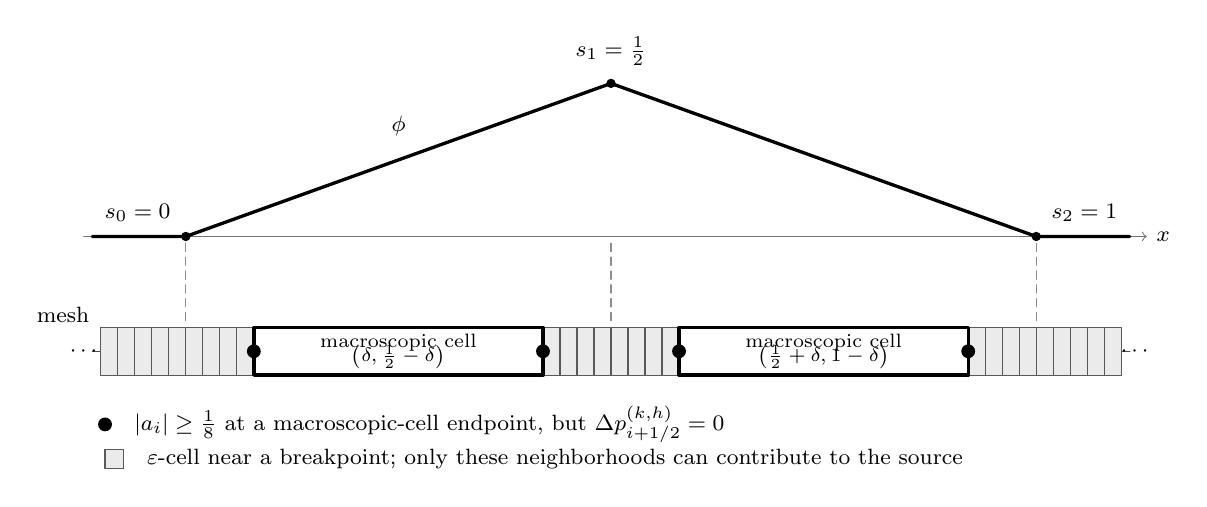
\begin{tikzpicture}[
				x=1.08cm,
				y=1.08cm,
				line cap=round,
				line join=round,
				every node/.style={font=\footnotesize}
				]
				\draw[->,black!55] (-1.20,1.35) -- (11.30,1.35)
				node[right,black] {$x$};
				\draw[very thick]
				(-1.10,1.35) -- (0,1.35) -- (5,3.15) -- (10,1.35) -- (11.10,1.35);
				\node[above left] at (2.70,2.42) {$\phi$};
				\fill (0,1.35) circle (1.7pt)
				node[above left=2pt] {$s_0=0$};
				\fill (5,3.15) circle (1.7pt)
				node[above=3pt] {$s_1=\frac12$};
				\fill (10,1.35) circle (1.7pt)
				node[above right=2pt] {$s_2=1$};
				
				\foreach \x in {0,5,10}
				\draw[densely dashed,black!45] (\x,1.27) -- (\x,0.36);
				
				\node[anchor=east] at (-1.02,0.43) {mesh};
				\draw[black!70] (-1.10,0) -- (11.10,0);
				
				\foreach \x in {-1.0,-0.8,-0.6,-0.4,-0.2,0,0.2,0.4,0.6}
				\draw[fill=black!8,draw=black!65] (\x,-0.28) rectangle +(0.2,0.56);
				\foreach \x in {4.2,4.4,4.6,4.8,5.0,5.2,5.4,5.6}
				\draw[fill=black!8,draw=black!65] (\x,-0.28) rectangle +(0.2,0.56);
				\foreach \x in {9.2,9.4,9.6,9.8,10.0,10.2,10.4,10.6,10.8}
				\draw[fill=black!8,draw=black!65] (\x,-0.28) rectangle +(0.2,0.56);
				
				\draw[fill=white,very thick] (0.8,-0.28) rectangle (4.2,0.28);
				\draw[fill=white,very thick] (5.8,-0.28) rectangle (9.2,0.28);
				\node[align=center,font=\scriptsize] at (2.5,0)
				{\scriptsize macroscopic cell\\[-3pt]$\bigl(\delta,\frac12-\delta\bigr)$};
				\node[align=center,font=\scriptsize] at (7.5,0)
				{\scriptsize macroscopic cell\\[-3pt]$\bigl(\frac12+\delta,1-\delta\bigr)$};
				
				\foreach \x in {0.8,4.2,5.8,9.2}
				\fill (\x,0) circle (2.5pt);
				
				\fill (-0.95,-0.86) circle (2.5pt);
				\node[anchor=west] at (-0.72,-0.86)
				{$|a_i|\ge\frac18$ at a macroscopic-cell endpoint, but
					$\Delta p_{i+1/2}^{(k,h)}=0$};
				\draw[fill=black!8,draw=black!65]
				(-0.95,-1.38) rectangle (-0.73,-1.16);
				\node[anchor=west] at (-0.57,-1.27)
				{$\varepsilon$-cell near a breakpoint; only these neighborhoods can
					contribute to the source};
				
				\node at (-1.18,0) {$\cdots$};
				\node at (11.18,0) {$\cdots$};
			\end{tikzpicture}%
		}
		\caption{The local two-scale pattern used in the fixed-mesh
			counterexample, shown schematically and not to scale.
			The filled dots mark four cell-average jumps bounded below
			independently of \(\varepsilon\).  Since each lies inside an affine region of \(\phi\), the
			corresponding reconstructed jump vanishes.  Only \(O_k(1)\) interfaces in the
			microscopic neighborhoods of the three breakpoints can contribute to the
			source.}
		\label{fig:nonuniform-tent-mesh}
	\end{figure}
	
	Both large cells have average $1/4$.  The microscopic cell immediately to
	the left of $(\delta,\frac12-\delta)$ has average at most $\delta$, whereas
	the one immediately to its right has average at least
	$\frac12-\delta$.  For the right large cell, the neighboring microscopic
	average is at least $\frac12-\delta$ on the left and at most $\delta$ on the
	right.  At each of these four interfaces, the corresponding jump
	$a_i$ therefore satisfies $|a_i|\ge\frac14-\delta\ge1/8$.  Hence
	\begin{equation}\label{eq:tent-jump-lower-bound}
		\sum_i|a_i|^{k+1}
		\ge4\left(\frac18\right)^{k+1}
		=:c_k>0.
	\end{equation}
	These four jumps occur where the cell size changes, not where the affine
	formula for $\phi$ changes.
	
	We next locate the interfaces at which the reconstructed jump can be
	nonzero.  Every possible order-$k$ reconstruction stencil for $I_q$ is a
	block of $k$ consecutive cells containing $I_q$.  Consequently, at
	$x_{i+1/2}$ every cell that can enter either one-sided reconstruction lies
	in
	\begin{equation}\label{eq:possible-stencil-hull}
		\mathcal K_i
		:=
		\{I_{i-k+1},I_{i-k+2},\ldots,I_{i+k}\}.
	\end{equation}
	Write $s_\alpha=x_{n_\alpha+1/2}$ and set
	\begin{equation}\label{eq:exceptional-interface-set}
		\mathcal A_\alpha
		:=
		\{i\in\mathbb Z:|i-n_\alpha|\le k\},
		\qquad
		\mathcal A
		:=
		\bigcup_{\alpha=0}^{2}\mathcal A_\alpha.
	\end{equation}
	In particular,
	\begin{equation}\label{eq:exceptional-set-cardinality}
		|\mathcal A|\le3(2k+1).
	\end{equation}
	
	If $i\notin\mathcal A$, then $\mathcal K_i$ contains no cells on opposite
	sides of any $s_\alpha$.  Indeed, if it crossed
	$s_\alpha=x_{n_\alpha+1/2}$, then
	\[
	i-k+1\le n_\alpha,
	\qquad
	i+k\ge n_\alpha+1,
	\]
	and hence $|i-n_\alpha|\le k-1$.  Thus all cells in $\mathcal K_i$ lie in a
	region on which $\phi$ is one affine function.
	
	Cell-average reconstruction reproduces affine functions when $k\ge2$.  To
	see this, suppose that $R\in\mathbb P_{k-1}$ and an affine function $\ell$
	have the same averages on $k$ consecutive cells.  A polynomial
	antiderivative of $R-\ell$ takes one value at the $k+1$ cell interfaces.
	After subtracting this common value, the antiderivative has $k+1$
	distinct zeros and degree at most $k$; hence
	it vanishes identically, and therefore $R=\ell$.  Both one-sided
	reconstructions at $x_{i+1/2}$ consequently agree with $\phi$ there, so
	\begin{equation}\label{eq:reconstructed-jump-off-exceptional-set}
		\Delta p_{i+1/2}^{(k,h)}=0,
		\qquad i\notin\mathcal A.
	\end{equation}
	In particular, the four large cell-average jumps in
	\eqref{eq:tent-jump-lower-bound} make no contribution to the source.
	
	It remains to estimate the interfaces in $\mathcal A$.  Fix
	$i\in\mathcal A_\alpha$.  If $I_q\in\mathcal K_i$, then
	\begin{equation}\label{eq:exceptional-hull-index-range}
		n_\alpha-2k+1\le q\le n_\alpha+2k.
	\end{equation}
	Because $N=10k$, every cell in this range has length $\varepsilon$ and lies
	in the microscopic neighborhood of the same point $s_\alpha$; it meets
	neither a large cell nor another point $s_\beta$.  If
	$c_\alpha:=\phi(s_\alpha)$, the $1$-Lipschitz continuity of $\phi$ gives
	\begin{equation}\label{eq:microscopic-average-bound}
		|\bar u_q-c_\alpha|
		\le C_k\varepsilon,
		\qquad I_q\in\mathcal K_i.
	\end{equation}
	Since $I_i,I_{i+1}\in\mathcal K_i$, this implies
	\begin{equation}\label{eq:small-jumps-near-breakpoints}
		|a_i|\le C_k\varepsilon,
		\qquad i\in\mathcal A.
	\end{equation}
	
	The same information controls both reconstructed traces.  Under the affine
	change of variables $x=s_\alpha+\varepsilon y$, each possible stencil in
	$\mathcal K_i$ becomes a block of $k$ unit cells.  For any fixed position of
	that block, evaluation of its cell-average reconstruction at the given
	interface is a linear functional of the $k$ cell averages.  After rescaling,
	the evaluation interface has only finitely many positions relative to such a
	block, depending on $k$ alone.  These finitely many linear functionals have a
	common norm bound.  Since constant data equal to $c_\alpha$ are
	reconstructed as the constant polynomial $c_\alpha$,
	\eqref{eq:microscopic-average-bound} yields
	\begin{equation}\label{eq:microscopic-trace-bound}
		|p_{i+1/2}^{-,(k,h)}-c_\alpha|
		+
		|p_{i+1/2}^{+,(k,h)}-c_\alpha|
		\le C_k\varepsilon,
		\qquad i\in\mathcal A_\alpha.
	\end{equation}
	This estimate holds for every possible reconstruction block and hence for
	the blocks selected by the ENO recursion.  Therefore
	\begin{equation}\label{eq:small-reconstructed-jumps}
		|\Delta p_{i+1/2}^{(k,h)}|
		\le C_k\varepsilon,
		\qquad i\in\mathcal A.
	\end{equation}
	Equations \eqref{eq:reconstructed-jump-off-exceptional-set},
	\eqref{eq:exceptional-set-cardinality},
	\eqref{eq:small-jumps-near-breakpoints}, and
	\eqref{eq:small-reconstructed-jumps} give
	\begin{equation}\label{eq:absolute-source-upper-bound}
		Q_{k,h}^{\mathrm{abs}}(\bar u)
		\le C_k\varepsilon^2.
	\end{equation}
	
	It remains to realize these estimates on one mesh.  For $n\ge1$, choose
	$\varepsilon_n\downarrow0$ so that
	$\delta_n:=N\varepsilon_n<1/8$, and put $y_n:=3n$.
	For each $n$, take the portion of the preceding local construction on
	$[-\delta_n,1+\delta_n]$ and translate it by $y_n$.  Thus the three
	intervals
	\[
	[y_n-\delta_n,y_n+\delta_n],\qquad
	[y_n+\tfrac12-\delta_n,y_n+\tfrac12+\delta_n],\qquad
	[y_n+1-\delta_n,y_n+1+\delta_n]
	\]
	are divided into cells of length $\varepsilon_n$, and the two intervening
	intervals are the macroscopic cells used above.  Join successive finite
	patterns by single cells and extend the mesh to the left, for instance by
	unit cells.  Since the patterns have length less than $5/4$ and the
	translation parameters $y_n$ are three units apart, all joining cells have
	positive length.
	The resulting set of interfaces is locally finite, and its increasing
	enumeration tends to $\pm\infty$.
	The joining-cell lengths are bounded below, whereas
	$\varepsilon_n\to0$; hence
	$\sup_{i,j\in\mathbb Z}h_i/h_j=\infty$.
	
	Let $\bar u^{(n)}$ be the cell averages on this fixed mesh of the
	translated tent $\phi_n(x):=\phi(x-y_n)$.  These data vanish outside the
	$n$th pattern.  Each breakpoint has $N=10k$ microscopic cells on either
	side.
	Hence, whenever the hull $\mathcal K_i$ in
	\eqref{eq:possible-stencil-hull} meets the support of $\phi_n$, every
	possible $k$-cell stencil at $x_{i+1/2}$ is contained in the $n$th pattern.
	Between the support of $\phi_n$ and either joining cell lie $N$ microscopic
	cells with zero averages, so every stencil meeting a joining cell
	reconstructs zero.  The locality argument above therefore applies without change and
	gives
	\[
	\sum_i|a_i^{(n)}|^{k+1}\ge c_k,\qquad
	\|\bar u^{(n)}\|_{\ell^\infty}\le\frac12,\qquad
	Q_{k,h}^{\mathrm{abs}}(\bar u^{(n)})
	\le C_k\varepsilon_n^2\longrightarrow0.
	\]
	For any finite $K$, these estimates contradict
	\eqref{eq:arbitrary-mesh-false-estimate} for all sufficiently large $n$.
	Thus no finite coercivity constant exists on this fixed mesh.
\end{proof}

This completes the proof of Theorem~\ref{thm:D}.  The fixed mesh just
constructed satisfies $\sup_{i,j\in\mathbb Z}h_i/h_j=\infty$; thus the
quasi-uniform estimate does not extend to arbitrary meshes without further
geometric assumptions.  Since the argument is uniform over all consecutive
$k$-cell stencils, it is independent of the stencil selected by ENO.


\appendix

\section{\texorpdfstring{An explicit functional for the fourth-order obstruction}{An explicit functional for the fourth-order obstruction}}
\label{app:fourth-order-functional}

This appendix defines the rational linear functional used in
Proposition~\ref{prop:fourth-order-obstruction} and proves the two identities
needed there.  The argument uses the nilpotent generator from
Lemma~\ref{lem:profile-exactness} and a direct comparison of coefficients.
We use the pullback endomorphism $T:=T_2^*$, determined on the coordinate
functions by
\begin{equation}\label{eq:appA-shift}
	Tu=u+c_0,\qquad
	Tc_0=c_0+c_1,\qquad
	Tc_1=c_1+c_2,\qquad
	Tc_2=c_2
\end{equation}
and, for $D\ge0$, the monomial basis
\begin{equation}\label{eq:appA-basis}
	\mathcal B_D
	:=\{u^ac_0^bc_1^cc_2^d:a,b,c,d\in\mathbb N_0,
	\ a+b+c+d=D\},
\end{equation}
ordered lexicographically with $u\succ c_0\succ c_1\succ c_2$.


On the polynomial algebra in $u,c_0,c_1,c_2$, let
$\mathcal N:=\log T$.  From \eqref{eq:appA-shift},
\begin{equation}\label{eq:appA-nilpotent-generator}
\mathcal N
=\left(c_0-\frac12c_1+\frac13c_2\right)\partial_u
\mathbin{+}\left(c_1-\frac12c_2\right)\partial_{c_0}
+c_2\partial_{c_1}.
\end{equation}
The operator on the right of
\eqref{eq:appA-nilpotent-generator} is a locally nilpotent derivation.  Its
exponential sends the four generators $u,c_0,c_1,c_2$ to the four expressions
in \eqref{eq:appA-shift}; hence its exponential is $T$, which proves
\eqref{eq:appA-nilpotent-generator}.  Let
$\mathcal N_7:=\mathcal N|_{\mathscr P_{2,7}}$.  Lemma~\ref{lem:profile-exactness}
gives
\begin{equation}\label{eq:appA-range-generator}
\operatorname{Range}\delta_{2,7}
=\operatorname{Range}\mathcal N_7.
\end{equation}

We recall the data defining the raw degree-seven profile mismatch and
its reduced form.  For
$f(u)=u^3/3$, the two-point flux and the fourth-order coefficients are
\begin{equation}\label{eq:appA-flux-data}
	F^*(u_L,u_R)
	=\frac{u_L^3+u_L^2u_R+u_Lu_R^2+u_R^3}{12},
	\qquad
	\alpha_1^{[2]}=\frac43,
	\qquad
	\alpha_2^{[2]}=-\frac16.
\end{equation}
Set
\begin{equation}\label{eq:appA-profile-flux}
	\mathcal F^{[2]}
	:=\frac43F^*(u,Tu)
	-\frac16\bigl(F^*(u,T^2u)+F^*(T^{-1}u,Tu)\bigr)
\end{equation}
and
\begin{equation}\label{eq:appA-Graw}
	G_{\mathrm{raw}}
	:=\bigl((Tu)^4-u^4\bigr)\mathcal F^{[2]}
	-\frac4{21}\bigl((Tu)^7-u^7\bigr).
\end{equation}
The coboundary removed in Section~\ref{sec:fourth-order-obstruction} is
generated by
\begin{equation}\label{eq:appA-H2}
	H_{\langle2\rangle}^{(7)}
	=-\frac13u^5c_0(c_0-c_1+c_2),
	\qquad
	\widetilde G^{(7)}
	=G_{\mathrm{raw}}-\delta_{2,7}H_{\langle2\rangle}^{(7)}.
\end{equation}


We now define a functional
$\mathfrak L\in\mathscr P_{2,7}^{*}$.  Its nonzero values on the monomial
basis $\mathcal B_7$ are listed below; it is zero on every monomial not
listed.
\begin{center}
	\small
	\begin{tabular}{@{}c r @{\qquad} c r@{}}
		\toprule
		$M$ & $\mathfrak L(M)$ & $M$ & $\mathfrak L(M)$\\
		\midrule
		$u^6c_0$ & $-180$ & $u^6c_1$ & $720$\\
		$u^6c_2$ & $1620$ & $u^5c_0c_1$ & $-90$\\
		$u^5c_0c_2$ & $-90$ & $u^5c_1^2$ & $240$\\
		$u^5c_1c_2$ & $-180$ & $u^4c_0^2c_1$ & $-12$\\
		$u^4c_0^2c_2$ & $36$ & $u^4c_0c_1^2$ & $72$\\
		$u^3c_0^3c_1$ & $-45$ & $u^2c_0^5$ & $60$\\
		\bottomrule
	\end{tabular}
\end{center}

For $a,b,c,d\in\mathbb N_0$ with $a+b+c+d=7$, put
$\lambda_{a,b,c,d}:=\mathfrak L(u^ac_0^bc_1^cc_2^d)$.  Extend this notation
to integer quadruples by setting $\lambda_{a,b,c,d}=0$ whenever any index is
negative.  Applying \eqref{eq:appA-nilpotent-generator} to a monomial of
total degree seven gives
\begin{align}
&\mathfrak L\!\left(\mathcal N_7
	u^ac_0^bc_1^cc_2^d\right)\notag\\
&\quad=a\left(
	\lambda_{a-1,b+1,c,d}
	-\frac12\lambda_{a-1,b,c+1,d}
	+\frac13\lambda_{a-1,b,c,d+1}\right)\notag\\
&\qquad+b\left(
	\lambda_{a,b-1,c+1,d}
	-\frac12\lambda_{a,b-1,c,d+1}\right)
	+c\lambda_{a,b,c-1,d+1}.
	\label{eq:appA-annihilation-recurrence}
\end{align}
Substitution of the values above into
\eqref{eq:appA-annihilation-recurrence} leaves eleven nontrivial cases, listed
below.
\begin{center}
	\small
	\begin{tabular}{@{}c l@{}}
		\toprule
		$(a,b,c,d)$ & terms remaining in \eqref{eq:appA-annihilation-recurrence}\\
		\midrule
		$(3,4,0,0)$ & $180-180$\\
		$(4,2,1,0)$ & $-180+144+36$\\
		$(4,3,0,0)$ & $90-36-54$\\
		$(5,0,2,0)$ & $360-360$\\
		$(5,1,0,1)$ & $180-180$\\
		$(5,1,1,0)$ & $-60-180+240+90-90$\\
		$(5,2,0,0)$ & $30+60-180+90$\\
		$(6,0,0,1)$ & $-540+540$\\
		$(6,0,1,0)$ & $-540-720-360+1620$\\
		$(6,1,0,0)$ & $270-180+720-810$\\
		$(7,0,0,0)$ & $-1260-2520+3780$\\
		\bottomrule
	\end{tabular}
\end{center}
Every displayed sum is zero.  Hence
$\mathfrak L\circ\mathcal N_7=0$, and
\eqref{eq:appA-range-generator} implies
\begin{equation}\label{eq:appA-annihilation}
	\mathfrak L\circ\delta_{2,7}=0.
\end{equation}

It remains to evaluate the functional on $G_{\mathrm{raw}}$.  If
$[M]P$ denotes the coefficient of a monomial $M$ in a polynomial $P$, direct
expansion of \eqref{eq:appA-Graw} gives
\begin{align}
\bigl(&[u^5c_0c_1]G_{\mathrm{raw}},
[u^5c_0c_2]G_{\mathrm{raw}},
[u^4c_0^2c_1]G_{\mathrm{raw}},
[u^4c_0^2c_2]G_{\mathrm{raw}},\notag\\[-2pt]
&[u^4c_0c_1^2]G_{\mathrm{raw}},
[u^3c_0^3c_1]G_{\mathrm{raw}},
[u^2c_0^5]G_{\mathrm{raw}}\bigr)\notag\\
&\qquad=
\left(-\frac23,\frac13,-\frac53,\frac5{18},-\frac49,
-\frac{22}{9},-\frac{17}{6}\right).
\label{eq:appA-Graw-coefficients}
\end{align}
The remaining five monomials in the support of $\mathfrak L$ have zero
coefficient in $G_{\mathrm{raw}}$.  Therefore
\begin{equation}\label{eq:appA-obstruction-pairing}
	\mathfrak L(G_{\mathrm{raw}})
	=60-30+20+10-32+110-170=-32.
\end{equation}
Equations \eqref{eq:appA-annihilation} and
\eqref{eq:appA-obstruction-pairing} are the two identities used in
Proposition~\ref{prop:fourth-order-obstruction}.  Since the term subtracted in
\eqref{eq:appA-H2} is a coboundary,
$\mathfrak L(\widetilde G^{(7)})=-32$.


\section{\texorpdfstring{Endpoint coefficients on quasi-uniform meshes}{Endpoint coefficients on quasi-uniform meshes}}
\label{app:quasi-uniform-estimates}

This appendix contains the endpoint-coefficient calculation used in
Lemmas~\ref{lem:nonuniform-endpoint-coefficients} and
\ref{lem:nonuniform-local-amplitude-bound}.  The localized source identity,
the moving-interpolant estimates, and the smooth-patching construction are
proved where they are used in Section~\ref{sec:mesh-geometry} and are not
repeated here.

Throughout the appendix, $k\ge2$ is fixed.  By
Lemma~\ref{lem:nonuniform-affine-scaling}, we work in normalized coordinates,
so that
\begin{equation}\label{eq:app-normalized-mesh}
	1\le h_i\le\Lambda
	\qquad(i\in\mathbb Z).
\end{equation}
All constants below are independent of the position of the local window and
of the data.  Their dependence on $k$ or on an intermediate difference order
$\ell$, and on $\Lambda$, is displayed explicitly.


\paragraph{Endpoint coefficients.}

We derive the endpoint coefficients used in
Lemmas~\ref{lem:nonuniform-endpoint-coefficients} and
\ref{lem:nonuniform-local-amplitude-bound}.  Write
\begin{equation}\label{eq:app-beta-expansion}
	D_j^{(\ell)}
	=\sum_{r=0}^{\ell-1}\beta_{j,r}^{(\ell)}a_{j+r},
	\qquad \ell\ge1.
\end{equation}
At the first level,
\[
\beta_{j,0}^{(1)}=\frac1{H_j^{(1)}}.
\]
The divided-difference recursion gives, with nonexistent terms understood to
be zero,
\begin{equation}\label{eq:app-beta-recursion}
	\beta_{j,r}^{(\ell+1)}
	=\frac{\beta_{j+1,r-1}^{(\ell)}-
		\beta_{j,r}^{(\ell)}}{H_j^{(\ell+1)}},
	\qquad 0\le r\le\ell.
\end{equation}
In particular, the two endpoint coefficients admit the explicit formulas
\begin{align}
	\beta_{j,0}^{(\ell)}
	&=\frac{(-1)^{\ell-1}}
	{\displaystyle\prod_{s=1}^{\ell}H_j^{(s)}},
	\label{eq:app-left-endpoint-coefficient}\\
	\beta_{j,\ell-1}^{(\ell)}
	&=\frac1{
		\displaystyle\prod_{s=1}^{\ell}H_{j+\ell-s}^{(s)}}.
	\label{eq:app-right-endpoint-coefficient}
\end{align}
In particular, both endpoint coefficients are nonzero.
Under \eqref{eq:app-normalized-mesh},
\begin{equation}\label{eq:app-endpoint-coefficient-lower-bound}
	|\beta_{j,0}^{(\ell)}|,
	|\beta_{j,\ell-1}^{(\ell)}|
	\ge \frac1{(\ell+1)!\Lambda^\ell}.
\end{equation}
All the coefficients are bounded uniformly as well.  For example, if
$C_{\ell,\Lambda}$ bounds the coefficients at level $\ell$, then
\eqref{eq:app-beta-recursion} and $H_j^{(\ell+1)}\ge\ell+2$ give
\[
\max_{0\le r\le\ell}
|\beta_{j,r}^{(\ell+1)}|
\le\frac{2C_{\ell,\Lambda}}{\ell+2}.
\]
Starting from $|\beta_{j,0}^{(1)}|\le1/2$ proves the required bound at every
fixed level.

Equations~\eqref{eq:app-left-endpoint-coefficient}--
\eqref{eq:app-endpoint-coefficient-lower-bound} give the endpoint
nondegeneracy used in Lemma~\ref{lem:nonuniform-local-amplitude-bound}. 
The induction itself, as well as all quasi-uniform interpolation and patching
estimates, is proved in Section~\ref{sec:mesh-geometry} at the point of use.


\begin{thebibliography}{99}

\bibitem{BLS}
Y. Brenier, C. De Lellis, and L. Sz\'ekelyhidi Jr.,
\emph{Weak--strong uniqueness for measure-valued solutions},
Comm. Math. Phys. 305 (2011), 351--361.

\bibitem{CayleySecondQuantics}
A. Cayley,
\emph{A second memoir upon quantics},
Philos. Trans. Roy. Soc. London 146 (1856), 101--126.

\bibitem{CFM2AN}
N. Chatterjee and U. S. Fjordholm,
\emph{Convergence of second-order, entropy stable methods for
multi-dimensional conservation laws},
ESAIM Math. Model. Numer. Anal. 54 (2020), 1415--1428.


\bibitem{DiPernaMV}
R. J. DiPerna,
\emph{Measure-valued solutions to conservation laws},
Arch. Rational Mech. Anal. 88 (1985), 223--270.

\bibitem{FjordholmThesis}
U. S. Fjordholm,
\emph{High-order accurate entropy stable numerical schemes for hyperbolic
conservation laws},
Ph.D. thesis, ETH Zurich, Diss. No.~21025, 2013.

\bibitem{FjordholmHandbook}
U. S. Fjordholm,
\emph{Stability properties of the ENO method},
in Handbook of Numerical Methods for Hyperbolic Problems: Basic and
Fundamental Issues, Handb. Numer. Anal. 17, Elsevier, 2016, pp.~123--145.

\bibitem{FKMT}
U. S. Fjordholm, R. K\"appeli, S. Mishra, and E. Tadmor,
\emph{Construction of approximate entropy measure-valued solutions for
hyperbolic systems of conservation laws},
Found. Comput. Math. 17 (2017), 763--827.

\bibitem{FMTtecno}
U. S. Fjordholm, S. Mishra, and E. Tadmor,
\emph{Arbitrarily high-order accurate entropy stable essentially
nonoscillatory schemes for systems of conservation laws},
SIAM J. Numer. Anal. 50 (2012), 544--573.

\bibitem{FMT}
U. S. Fjordholm, S. Mishra, and E. Tadmor,
\emph{ENO reconstruction and ENO interpolation are stable},
Found. Comput. Math. 13 (2013), no.~2, 139--159,
\href{https://doi.org/10.1007/s10208-012-9117-9}{doi:10.1007/s10208-012-9117-9}.

\bibitem{FultonHarris}
W. Fulton and J. Harris,
\emph{Representation Theory: A First Course},
Graduate Texts in Mathematics 129, Springer, 1991.


\bibitem{Harten}
A. Harten, B. Engquist, S. Osher, and S. R. Chakravarthy,
\emph{Uniformly high order accurate essentially non-oscillatory schemes, III},
J. Comput. Phys. 71 (1987), 231--303.

\bibitem{HiltebrandMishra}
A. Hiltebrand and S. Mishra,
\emph{Entropy stable shock capturing space--time discontinuous Galerkin
schemes for systems of conservation laws},
Numer. Math. 126 (2014), 103--151.

\bibitem{JiangShu}
G.-S. Jiang and C.-W. Shu,
\emph{Efficient implementation of weighted ENO schemes},
J. Comput. Phys. 126 (1996), 202--228.

\bibitem{Kruzkov}
S. N. Kruzhkov,
\emph{First order quasilinear equations in several independent variables},
Math. USSR-Sb. 10 (1970), 217--243.


\bibitem{LMR}
P. G. LeFloch, J.-M. Mercier, and C. Rohde,
\emph{Fully discrete, entropy conservative schemes of arbitrary order},
SIAM J. Numer. Anal. 40 (2002), 1968--1992.

\bibitem{LiWuCompanion}
Z. Li and K. Wu,
\emph{Compactness and convergence theory for entropy stable ENO schemes 
of arbitrarily high order},
preprint, 2026.

\bibitem{LPT}
P.-L. Lions, B. Perthame, and E. Tadmor,
\emph{A kinetic formulation of multidimensional scalar conservation laws and
related equations},
J. Amer. Math. Soc. 7 (1994), 169--191.

\bibitem{LiuOsherChan}
X.-D. Liu, S. Osher, and T. Chan,
\emph{Weighted essentially non-oscillatory schemes},
J. Comput. Phys. 115 (1994), 200--212.

\bibitem{MajidTomasic}
S. Majid and I. Toma\v{s}i\'c,
\emph{On braided zeta functions}, 
Bull. Math. Sci. 1 (2011), 379--396.

\bibitem{Nirenberg}
L. Nirenberg,
\emph{On elliptic partial differential equations},
Ann. Scuola Norm. Sup. Pisa Cl. Sci. (3) 13 (1959), no.~2, 115--162.


\bibitem{Schumaker}
L. L. Schumaker,
\emph{Spline Functions: Basic Theory}, 3rd ed.,
Cambridge Mathematical Library, Cambridge University Press, 2007.

\bibitem{Shu}
C.-W. Shu,
\emph{Essentially non-oscillatory and weighted essentially non-oscillatory
schemes for hyperbolic conservation laws},
in Advanced Numerical Approximation of Nonlinear Hyperbolic Equations,
Lecture Notes in Math. 1697, Springer, 1998, pp.~325--432.


\bibitem{StanleyEC1}
R. P. Stanley,
\emph{Enumerative Combinatorics, Vol. 1}, 2nd ed.,
Cambridge Studies in Advanced Mathematics 49, Cambridge University Press,
2012.

\bibitem{TadmorTao}
E. Tadmor and T. Tao,
\emph{Velocity averaging, kinetic formulations, and regularizing effects in
quasi-linear PDEs},
Comm. Pure Appl. Math. 60 (2007), 1488--1521.

\bibitem{ZakerzadehMay}
M. Zakerzadeh and G. May,
\emph{On the convergence of a shock capturing discontinuous Galerkin method
for nonlinear hyperbolic systems of conservation laws},
SIAM J. Numer. Anal. 54 (2016), 874--898.

\end{thebibliography}

\end{document}
